%% -----------------------------------------------------------------
%%  Original Template
%% -----------------------------------------------------------------
%%
%%  
\documentclass[11pt,a4paper, final]{report}

\makeindex

\PassOptionsToPackage{nottoc}{tocbibind}

% Include the style file which contains all the required formatting
% information that is set out in the Research Higher Degrees Resource
% Handbook (2003 version). NOTE: This file uses the following packages
% 'graphicx' for graphics manipulation
% 'fancyhdr' for nice headers and footers.
% 'makeidx' for generating the index
% 'tocbibind' for adding table of contents entries for bibliography, index etc.
% 'sectsty' for generating stylised chapter and section headings.
% 'lipsum' for generating dummy text.
% 'natbib' and 'har2nat' for bib citations.
% 'xcolor' color package.
% 'epstopdf' EPS to PDF conversion.
\usepackage{Packages/mathphdthesis}



\includeonly{
Frontbackmatter/prelude 	% Contains all the relevant candidate information (name, degrees, abstract etc)
,Frontbackmatter/newcom 	% Place all you new commands in here
,Nomenclature/nomenclature  % The nomenclature chapter
,Chapters/Chapter1/chap1
,Chapters/Chapter2/chap2
,Chapters/Chapter3/chap3
,Chapters/Chapter4/chap4
,Chapters/Chapter5/chap5
,Chapters/Chapter6/chap6
,Appendices/app0   			% Needed to switch to appendix mode
,index  					% Places the index in the thesis
}

% Begin the thesis
\begin{document}
	% Include all the pieces of your thesis in here
	% prelude.tex (specification of which features in `mathphdthesis.sty' you
% are using, your personal information, and your title & abstract)

% Specify features of `mathphdthesis.sty' you want to use:
\titlepgtrue 												% Main title page (required)
\signaturepagetrue 											% Page for declaration of originality (required)
\copyrighttrue 												% Copyright page (required)
\abswithesistrue 											% Abstract to be bound with thesis (optional)
\dedicatetrue 											% Dedicaiton

\acktrue 													% Acknowledgments page (optional)
\publicationtrue										    	% Publications  page (optional)
\tablecontentstrue 											% Table of contents page (required)
\tablespagetrue 											% Table of contents page for tables (required only if you have tables)
\figurespagetrue 											% Table of contents page for figures (required only if you have figures)

% Title, author, supervisors, university, date of submission
\title{Feasibility study of artificial intelligence approach for delamination identification in composite laminates}							% Thesis title
\author{Abdalraheem A. Ijjeh} 	% First name and surname of candidate (e.g. John Doe)
\prevdegrees{M.Sc. Eng.}              			% Specify your previous degrees (e.g. B.E. (Hons))
\institute{Mechanics of Intelligent Structures Department}								% Institute of department (e.g. National Centre for Maritime Engineering and Hydrodynamics)

\submittedfor{A dissertation submitted to the Scientific Board of the Szewalski Institute of Fluid-Flow Machinery, Polish Academy of Sciences in partial fulfillment of the requirements for the Degree of Doctor of Philosophy}			% Degree thesis is submitted for (e.g. Submitted in fulfillment of the requirements for the Degree of Doctor of Philosophy)
\advisor{ Pawe\l{} Kudela, D.Sc. Ph.D. Eng.} % Supervisors: (e.g. Prof. Lawrence K. Forbes)
\dept{The Szewalski Institute of Fluid-Flow Machinery, Polish Academy of Sciences}
\date{May, 2022}

% Dedicaton page
\newcommand{\dedication}
{
	\begin{center}
		\emph{To my beloved family.}
	\end{center}
}
% Acknowledgments page
\newcommand{\acknowledgement}
{
I would like to express my deepest sense of gratitude to my supervisor, Prof.~Pawe\l{} Kudela, for his guidance, encouragement, and advice from the initial stage of my Ph.D. studies till the end of helping me develop a thorough understanding of the subject and my studies.
Also, I would like to thank him for passing me his expertise and knowledge of being a scientific researcher.

I would like to express my gratitude to Dr.~Maciej Radzienski for supplying the experimental data of the full wavefield measured by SLDV.

I would like to thank my committee members for letting my defense be a good moment of time, and for their constructive comments and suggestions.

My sincere thanks to my father, Dr.~Abdullah Ijjeh, for his continuous guidance, advice, and encouragement throughout my studies.

I would like to thank my mother for her endless love, trust, encouragement, and support throughout my life.

I would like to thank my wife, Duaa, and my daughter, Raghad, for their consistent support and encouragement.

I would like to thank my brother, Dr.~Abdalraheman Ijjeh, for his consistent advice.

And finally, I would like to thank everyone who supported me during my journey of Ph.D. studies.

}

% Abstract to be bound with thesis
\newcommand{\abstextwithesis}
{
	%Basic abstract goes here. Can use paragraphs and normal \LaTeX commands.
	...
}

% Puplications page
\newcommand{\publications}
{
	\textbf{Journal papers}
	\begin{itemize}
		\item Ijjeh, Abdalraheem A., Saeed Ullah, and Pawel Kudela. \enquote{Full wavefield processing by using FCN for delamination detection.} Mechanical Systems and Signal Processing 153 (2021): 107537.
		\item Ijjeh, Abdalraheem A., and Pawel Kudela. \enqoute{Deep learning based segmentation using full wavefield processing for delamination identification: A comparative study.} Mechanical Systems and Signal Processing 168 (2022): 108671.
		\item  Saeed Ullah, Ijjeh, Abdalraheem A., and Pawel Kudela. \enquote{Deep learning approach for delamination identification using animation of Lamb waves.} Structural Health Monitoring, SAGE (Under review)
		\item Abdalraheem Ijjeh, Saeed Ullah, Maciej Radzienski and Pawel Kudela. \enqoute{Deep learning super-resolution for the reconstruction of full wavefield of Lamb waves}. Mechanical Systems and Signal Processing (Under review).
	\end{itemize}
	\par\medskip
	\textbf{Conference papers}
	\begin{itemize}
		\item Ijjeh, A., Kudela, P. Feasibility Study of Full Wavefield Processing by Using CNN for Delamination Detection. Proceedings of the International Conference on Structural Health Monitoring of Intelligent Infrastructure, Porto, Portugal, 30 June - 2 July 2021, ISSN 2564-3738, pages \(709-713\).
		\item Ijjeh, A., Kudela, P. (2023). Delamination Identification Using Global Convolution Networks. In: Rizzo, P., Milazzo, A. (eds) European Workshop on Structural Health Monitoring. EWSHM 2022. Lecture Notes in Civil Engineering, vol 270. Springer, Cham. https://doi.org/10.1007/978-3-031-07322-9\_5
	\end{itemize}
	\par\medskip
	\textbf{Scientific monographs}
	\begin{itemize}
		\item Abdalraheem Ijjeh [100\%], Machine Learning for SHM: Literature Review, chapter in: Wybrane zagadnienia inżynierii mechanicznej, Praca zbiorowa pod redakcją M. Mieloszyk, T. Ochrymiuka, Wydawnictwo Instytutu Maszyn Przepływowych PAN, Gdańsk, 2020, ISBN 978-83-88237-97-3, [80 pt].
		\item Abdalraheem Ijjeh [100\%], Data-driven based approach for damage detection, chapter in: Wybrane zagadnienia inżynierii mechanicznej 2021, Praca zbiorowa pod redakcją M. Mieloszyk, T. Ochrymiuka, Wydawnictwo Instytutu Maszyn Przepływowych PAN, Gdańsk, 2021, ISBN 978-83-66928-00-8 , [80 pt].
		\item Abdalraheem Ijjeh [100\%], Deep Learning based Damage Imaging
		techniques, chapter in: Wybrane zagadnienia inżynierii mechanicznej 2022, Praca zbiorowa pod redakcją M. Mieloszyk, T. Ochrymiuka, Wydawnictwo Instytutu Maszyn Przepływowych PAN, Gdańsk, 2022, ISBN 000-00-00000-00-0 , [80 pt].
	\end{itemize}
	\par\medskip
	\textbf{Internships during study}
	\begin{itemize}
		\item Erasmus+ (Wave propagation in phononic crystals, 05/06/2022 – 10/06/2022)	ISEN-JUNIA (CNRS-IEMN) (Lille, France).
%		\begin{itemize}
%			\item Training on the fundamentals of phononic crystals.
%			\item Training on the basics of the Finite Element software "COMSOL Multiphysics"
%			\item Training on the meshing procedure of the periodic unit cells.
%			\item Training on the parametrization of wavenumbers in the eigenvalue problems for the calculation of dispersion diagrams in the first irreducible Brillouin zone.
%			\item Training on the computation of the dispersion diagrams by using "COMSOL Multiphysics"
%		\end{itemize}
		 
	\end{itemize}

}


% Engineering guote page
\newcommand{\engineeringquote}
{
\null\vskip1.8in
\begin{quote}
\begin{flushright}
\end{flushright}
\end{quote}
}

% Bibliography Title
\renewcommand{\bibname}{References/Bibliography}
% Bibliography spacing
\setlength\bibitemsep{1.5\itemsep}

% Settings for array package
\newcolumntype{L}[1]{>{\raggedright\let\newline\\\arraybackslash\hspace{0pt}}m{#1}}
\newcolumntype{C}[1]{>{\centering\let\newline\\\arraybackslash\hspace{0pt}}m{#1}}
\newcolumntype{R}[1]{>{\raggedleft\let\newline\\\arraybackslash\hspace{0pt}}m{#1}}

% Take care of things in `mathphdthesis.sty' behind the scenes.
% Basically just does a check of all the fields that have been activated

% above and fills out the appropriate pages and adds them to the thesis.
\beforepreface
\afterpreface
	% newcom.tex (new command definitions)

% Some examples (yours may be different):
\newtheorem{theorem}{Theorem}[section]
\newtheorem{lemma}[theorem]{Lemma}
\newcommand{\bfx}{{\ensuremath{\mathbf{x}}}}

	% chap9.tex (Chapter 9 of the thesis)

%\chapter[NOMENCLATURE]{NOMENCLATURE}
% Overwrite TOC chapter title
\chapter*{NOMENCLATURE}
\addcontentsline{toc}{chapter}{NOMENCLATURE}
\label{nomenclature}
%
%% -----------------------------------------------------------------------------------------------------------------
%% Greek symbols
%% -----------------------------------------------------------------------------------------------------------------
%
%% GENERAL CONSTANTS
%\nomtypeG{\( \lambda \)}{Full scale to model scale ratio}{$\frac{L_{s}}{L_{m}}$}{-}
%
%% -----------------------------------------------------------------------------------------------------------------
%% Dimensionless numbers
%% -----------------------------------------------------------------------------------------------------------------
%
%\nomtypeD{\( \mathcal A_r \)}{Archimedes number}{\(\displaystyle\frac{d^3g\rho_c\abs{\Delta\rho}}{\mu_c^2} = \sqrt{\frac{\mathcal E_0^3}{\mathcal M_0}} \)}
%
%% -----------------------------------------------------------------------------------------------------------------
%% Roman symbols
%% -----------------------------------------------------------------------------------------------------------------
%
%% AREAS 
%\nomtypeR[AN]{A\textsubscript{N}}{Nozzle discharge area}{-}{m\textsuperscript{2}}
%
%% DIMENSIONS
%\nomtypeR[T]{T}{Draft}{-}{$m$}
%
%\printnomenclature[6em]
%%\printnomenclature[2cm]

	% Set page numbering to arabic the first time we commence a chapter.
% This is required to get the page numbering correct.
\pagenumbering{arabic}

% Note that the text in the [] brackets is the one that will
% appear in the table of contents, whilst the text in the {}
% brackets will appear in the main thesis.

%% CHAPTER HEADER /////////////////////////////////////////////////////////////////////////////////////
\chapter[Introduction]{Introduction}
\label{ch1}

%% CHAPTER INTRODUCTION ///////////////////////////////////////////////////////////////////////////////

%\lipsum[1]

%% INCLUDE SECTIONS ///////////////////////////////////////////////////////////////////////////////////

\section{Problem Definition}
\label{sec11}
Carbon fibre reinforced plastics (CFRP) materials have a wide range of applications in different industries due to their characteristics such as high strength, low density, resistance to fatigue and corrosion.
Moreover, composite structures are exposed to different types of operating conditions during their service life, such as temperature variations and cyclic loading, which ultimately results in initiating damage. 
However, composite structures are subject to several operating conditions (such as temperature variations and cyclic loading) during their service life, which eventually can initiate fatigue damage in the composite structures.
Furthermore, damage mechanisms in composite structures are more complex than those in conventional metallic structures due to the multi-layer property and general anisotropy~\cite{Wu2021}. 

One of the main damage types developed in composite structures is inter-laminar delamination.
Delamination is developed from matrix micro-cracks in a nonlinear manner with the application of cyclic loading~\cite{Reifsnider1983, Wu2021}, which can alter the compression strength of composite laminates and gradually affect the composite structure to encounter failure by buckling. Therefore, it can seriously decrease the performance of composite structures.
Consequently, delamination identification in its early stages can significantly help to avoid catastrophic structural collapses.

Various approaches of non-destructive evaluation (NDE) and structural health monitoring (SHM) have been utilised for damage detection in composite structures. 
Further, such approaches can be divided into two categories: model-based approaches and data-driven approaches.

The model-based approaches for SHM aim to reflect the process of damage development in composite materials by implementing a physics-based numerical model and introducing necessary variables to adjust the model to fit the actual application scenario ~\cite{Wu2021}. 
However, model-based approaches have practical shortcomings that restrict their suitability to simple structures under well-controlled environments.
%%%%%%%%%%%%%%%%%%%%%%%%%%%%%%%%%%%%%%%%%%%%%%%%%%%%%%%%%%%%%%%%%%%%%%%%%%%%%%%%
%--- Need to be written in my own words
%%%%%%%%%%%%%%%%%%%%%%%%%%%%%%%%%%%%%%%%%%%%%%%%%%%%%%%%%%%%%%%%%%%%%%%%%%%%%%%%
%A lot of research has been conducted in materials properties identification mainly using vibration-based methods and Ultrasonic Guided Wave (UGW) based methods [1]. 
%The vibration-based technique is global in nature and is sensitive to boundary conditions which make it difficult for its application in in-situ health monitoring [2]. 
%Meanwhile the UGW’s are highly sensitive to lamina properties that has enabled researchers to use them in various non-destructive evaluations (NDE) and structural health monitoring (SHM) tasks [3][4][5]. 
%
%However, guided waves are multi-modal waves and using them for material properties identification often includes a great deal of signal processing expertise.
%
%However,extracting robust damage indicators from the measured UGW signals is extremely challenging because of its complex UGW propagation characteristics (e.g., dispersion, multi-mode, and mode conversion), which is further exacerbated in composite structures.
%%%%%%%%%%%%%%%%%%%%%%%%%%%%%%%%%%%%%%%%%%%%%%%%%%%%%%%%%%%%%%%%%%%%%%%%%%%%%%%%
On the other hand, the data-driven approaches for SHM utilise registered data from the structure under different structural states and perform an analysis using data analysis methods.
Data-driven approaches that utilise artificial intelligence methods such as deep learning are getting more popular due to the recent advancements in sensing technology.
Hence, the deep learning-based approach revealed new dimensions for resolving problems and offered the opportunity for being implemented and integrated with the NDE and further with SHM approaches. 
Consequently, applying deep learning techniques can handle issues regarding data preprocessing and feature extraction.
Nowadays, end-to-end approaches are developed, in which unprocessed data are fed into the model.
Hence, the model will learn to recognise the patterns and detect the damage.
%Accordingly, deep learning (DL) techniques employed for damage detection and localisation are able to handle large data registered in a complex real-world structures.
%%%%%%%%%%%%%%%%%%%%%%%%%%%%%%%%%%%%%%%%%%%%%%%%%%%%%%%%%%%%%%%%%%%%%%%%%%%%%%%%
%--- Need to be written in my own words
%%%%%%%%%%%%%%%%%%%%%%%%%%%%%%%%%%%%%%%%%%%%%%%%%%%%%%%%%%%%%%%%%%%%%%%%%%%%%%%%
%
%Recently, data-driven approaches using machine learning (ML) algorithms and statistical models have been developed for SHM due to their robust information fusion and pattern analysis capabilities [19–22]. 
%These capabilities can be leveraged for analyzing and extracting damage sensitive features for effective damage detection and classification [23–30]. 

%Larrosa et al., [26] proposed a damage diagnosis framework using ultrasonic Lamb waves and Gaussian discriminant analysis (GDA) to classify fatigue damage modes that developed in a CFRP plate structure with increasing fatigue cycles. Damage sensitive features, such as time-of-flight (ToF), amplitude, energy, and PSD, were extracted from the first arrival wave packet, and the patterns in the features were analyzed using a trained GDA model to classify matrix cracking and delamination. 
%The results were validated using X-ray images, showing accurate damage classification capabilities. 
%Fendzi et al., [27] developed a Lamb wave-based SHM framework integrated with a Bayesian approach to localize damage in CFRP composite structures. 
%The Bayesian inference was used to quantify experimental uncertainties in the angle dependent group velocity estimation while demonstrating good damage localization capabilities in both CFRP composite plate and
%sandwich panel. 
%
%Even though there are many data-driven SHM methodologies available in the literature, the diagnostic capabilities of these techniques may be limited due to the extensive process of manual or signal processing-based damage feature extraction that may not be applicable.

%% SECTION HEADER /////////////////////////////////////////////////////////////////////////////////////
\section{Example: Equations}
\label{sec12}

%% SECTION CONTENT ////////////////////////////////////////////////////////////////////////////////////

This section shows a few equation examples. Labels can be used to reference equations.
\begin{itemize}
	\item Example (Equation \ref{eq:1_1})
	\item Example (Equation \ref{eq:1_2})
	\item Example (Equation \ref{eq:1_3})
	\item Example (Equation \ref{eq:1_4})
	\item Example (Equation \ref{eq:1_5})
\end{itemize}

\begin{equation}
\label{eq:1_1}
\overline{M}_{i}=\iint\limits_A \rho\;u_{i}\left(u_{k}\;n_{k} \right)\;dA
\end{equation}

\begin{equation}
\label{eq:1_2}
V_{REF} = \left( \frac{2 \times 144 \times P_{DYN}}{\rho} \right)^{\frac{1}{2}}
\end{equation}

\begin{equation}
\label{eq:1_3}
V_{MOM} = \left( \frac{A_{TIP} (\frac{V_{REF}}{2})^{2} + A_{MIDDLE} V_{REF}^{2} + A_{HUB} V_{HUB}^{2}}{A_{JET} V_{AVG}} \right)
\end{equation}

\begin{equation}
\label{eq:1_4}
\begin{aligned}
& Q_{J}= \int_0^\delta Vdy+\left(y-\delta \right)b\;V_{s}\\
& Q_{J}= b\;V_{s} \int_0^\delta \left(\frac{y}{\delta} \right)^\frac{1}{n}dy+\left(y-\delta \right)b\;V_{s}\\
& Q_{J}=\frac{b\;V_{s}}{\left(\frac{n+1}{n} \right)}\delta+\left(y-\delta \right)b\;V_{s}\\
& Q_{J}=b\;V_{s}\left(y-\frac{\delta}{n+1} \right)
\end{aligned}
\end{equation}

\begin{equation}
\label{eq:1_5}
B_{K_{T_{Jx}}}=\sqrt{\left(\theta_{Q_{J}}B_{Q_{J}} \right )^{2}+\left(\theta_{D}B_{D} \right )^{2}+\left(\theta_{n}B_{n} \right )^{2}+\left(\theta_{ \alpha }B_{ \alpha } \right )^{2}+\left(\theta_{\rho}\left(B_{\rho}+\theta_{\rho tw}B_{tw} \right ) \right )}
\end{equation}

\section{Objectives and motivations}
\label{sec13}

The main objective of the work is to develop an artificial intelligence (AI) driven diagnostic system for delamination identification in composite laminates.
Furthermore, to explore the potential of utilising artificial intelligence-based approaches to investigate damage detection and identification based on the propagation of Lamb waves.
Data corresponding to elastic wave propagation has very complex patterns of wave reflections. 
It is difficult to explicitly program instructions that will output a damage map of an element of a structure based on anomalies in propagating elastic waves (e.g., reflections from discontinuities).
Hence, this research aims to explore possible solutions that employ deep neural networks (DNN), as they are promising approaches.
The progress in the machine learning field in the last decade, along with increasing computation power capabilities, makes it a perfect time to investigate potential applica\-tions of DNN. 
DNN is an emerging tool that has successful applications in computer vision and speech recognition, among other applications. 
Nowadays, certain neural network (NN) architectures surpass human-level accuracy in image classification. 
The main advantage of DNN in comparison to other machine learning approaches is scalability. 
It means that the performance of DNN increases with NN size as well as the size of the dataset used for supervised learning.

\textbf{Therefore, it is possible to use an end-to-end approach in which DNN processes the animation of propagating waves (input) directly into a damage map (output).}

Another objective of this research is to address the issue of slow data acquisition of high-resolution full wavefields of Lamb wave propagation.
Hence, to overcome such an issue, I aim to develop a deep learning system capable of recovering the high-resolution frames of Lamb wave propagation and their interaction with delamination and boundaries from low-resolution measurements with high accuracy.
Consequently, such a system will speed up the data acquisition process.


This research will help answer legitimate questions regarding the utilisation of deep learning techniques by processing the full wavefield of propagating elastic waves for delamination identification in composite laminates:
\begin{itemize}
	\item Can the proposed AI-driven diagnostic model be more accurate than the conven\-tional signal processing technique?
	\item Knowing that experimental signals contain noise, is it adequate to use a numerical model for generating a dataset?
	\item Can a technique such as data augmentation enhance the training of deep learning models?
	\item How well can deep learning models generalise to new unseen data? Further, to experimental data acquired by SLDV?
	\item Is it computationally feasible to utilise all frames of propagating waves, or can utilisation of certain frames be efficient enough?
	\item Does the implementation of different deep learning architectures result in different accuracies in damage identification? Is the comparison metric among these architectures sufficient for determining the efficient one?
	\item Do deep learning techniques for delamination identification utilised in this thesis have any potential for practical applications in the long term?
	\item Can deep learning techniques developed for super-resolution image reconstruction be used to recover the high-resolution full wavefield frame from the low-resolution measurements with adequate accuracy to detect the damage?
\end{itemize}

\section{Thesis contribution}
\label{sec14}
The main novelty of this work consists of applying for the first time a full wavefield data of elastic waves propagation (numerically generated dataset) as an input to various supervised deep neural networks, which is capable of identifying damage.

	\chapter[Literature Review]{Literature Review}
\label{ch2}
Structural health monitoring (SHM) intends to describe a real-time evaluation 
of the materials of a structural component or the full construction during the structure life-cycle~\cite{Balageas2010}. 
Furthermore, SHM supports detecting and characterising defects in structures 
as a whole or in their parts.
Detection of structural defects is critical because they may impair the safety of the structure during its operation~\cite{Yuan2016}. 

The purpose of SHM is to distinguish any potential change that occurs at a structure that could decay the performance of the entire system at the earliest possible time so that an action can be taken to reduce the downtime, operational costs and maintenance costs, consequently reducing the risk of 
catastrophic failure, injury, or even loss of life.
Moreover, SHM improves the work organization of maintenance services replacing scheduled and periodic maintenance inspection with performance-based maintenance.
It decreases maintenance labour, in particular, by avoiding dismounting undamaged parts and through reducing the individual involvement~\cite{Balageas2010}.

We can look at SHM as an improved method to perform Non-Destructive Evaluation (NDE). 
Nonetheless, SHM involves sensors that are integrated into structures, data transmission, computational power, and processing ability within structures~\cite{Balageas2010}. 
The typical organization of an SHM system is depicted in Fig.~\ref{fig:SHMsystem}. 
Such a system is built from a diagnostic part (low level) and a prognosis part (high level).
The diagnostic part is responsible for the detection, localization, and evaluation of any damage.
The prognosis part includes the production of information concerning the outcomes of the diagnosed damage.
%%%%%%%%%%%%%%%%%%%%%%%%%%%%%%%%%%%%%%%%%%%%%%%%%%%%%%%%%%%%%%%%%%%%%%%%%%%%%%%%
\begin{figure} [!ht]
	\begin{center}
		\includegraphics[width=1\textwidth]{Figures/Chapter_1/SHM_system.png}
	\end{center}
	\caption{Organization of SHM systems.} 
	\label{fig:SHMsystem}
\end{figure}
%%%%%%%%%%%%%%%%%%%%%%%%%%%%%%%%%%%%%%%%%%%%%%%%%%%%%%%%%%%%%%%%%%%%%%%%%%%%%%%%
In general, we can categorize SHM strategies into two main schemes, local and global schemes. 
Local schemes were discussed in ~\cite{Grimberg2001,Raghavan2007}
and global schemes were discussed in~\cite{Adams2002,Doebling1998,Uhl2004}. 
Local schemes aim at monitoring a small area of the structure enclosing the transducers that are used for registering the data signals after the structure is exited. 
For this purpose, a few phenomena are used like ultrasonic waves~\cite{Raghavan2007}, eddy currents~\cite{Grimberg2001}, and acoustic emission~\cite{Grosse2008}. 
On the other hand, global schemes are related to the global behaviour of the structure~\cite{Balageas2010}. 
For this purpose, vibration techniques are utilized which can be classified as signal-based and model-based.
Signal-based approaches analyse measured responses of the structure after 
ambient excitation in order to identify possible defects~\cite{Stepinski2013}. 
The model-based approaches use various types of models of a monitored structure 
to detect and localize damage in the structure by utilising relations 
between the model parameters and distinct damage features~\cite{Stepinski2013}. 
%%%%%%%%%%%%%%%%%%%%%%%%%%%%%%%%%%%%%%%%%%%%%%%%%%%%%%%%%%%%%%%%%%%%%%%%%%%%%%%%
%% SECTION HEADER ////////////////////////////////////////////////////////////////////////////////
\section[SHM for composite materials]{SHM for composite materials}
\label{sec21}
Composite materials are widely used in various industries, due to their useful characteristics. 
A composite material can be described as a compound of two or more different materials to acquire new features that cannot be achieved by specific components functioning individually.
Distinct from metallic alloys, which are isotropic materials, each material in the composite has its characteristics~\cite{Campbell2010}.
Accordingly, several advantages of these various characteristics can be obtained. 
Generally, composite materials are categorized into~\cite{Jones1999}:
\begin{itemize}
	\item Fibre-reinforced composite materials consisting of three parts: the fibres as the discontinuous phase, the matrix as the continuous phase, and the fine inter-phase region, also known as the interface~\cite{Cantwell1991}.
	\item Laminated composite materials are an assembly of multiple layers of fibre-reinforced or fabric-reinforced composite materials (e.g. plain weave, twill) that can be combined to implement necessary design features~\cite{Ramirez1999}.
	\item Particulate composite materials are characterized as being composed of particles suspended in a matrix (e.g. composite with short fibres).
\end{itemize}

When comparing composite materials to regular metallic materials, we can notice that composites have some advantages over metallic materials. 
The advantages can be summarized as~\cite{Campbell2010}:
\begin{itemize}
	\item low density with high strength and stiffness,
	\item high vibration damping capacity, and more temperature resistance,
	\item strong texture in micro-structures, making it easy to design and satisfy different application needs, 
	\item chemical and corrosion resistance.	
\end{itemize}

However, composite materials possess some disadvantages.
Due to the nature of multiphase materials, composite materials present anisotropic characteristics. 
It is considered a disadvantage in the case of wave propagation due to the complexity of processing of registered signals. 
%Their material capacities, mainly associated with manufacturing processes, are dispersive~\cite{Awad2012}. 

Damage can accidentally occur in composite materials, either during the process of manufacturing or during the regular service life of the structure. 
The lack of reinforcement in the out-of-plane direction causes that composite materials are susceptible to impact damage~\cite{Cai2012}. 
Under a high energy impact, little penetration rises in composite materials.  
Furthermore, low to medium energy impact can initiate delamination which is caused by bending cracks, matrix cracking, and shear cracks,  which mostly happen below the top surfaces and are barely visible~\cite{Cai2012}. 
Delamination can alter the compression strength of composite laminate, and it will gradually affect the composite to encounter failure by buckling~\cite{NurAzrieBtSafri2018}.
The tension encountered by the composite structure creates cracks and produces delamination between the laminates, which leads to more damage~\cite{NurAzrieBtSafri2018}. 
Furthermore, when a composite laminate encounters low- or high-velocity impact, various damage modes can appear, including fibre crack, matrix crack, delamination and fibre pullout. 
All of these damage modes are dependent on the impact parameter such as impact energy and impactor mass or impactor shape~\cite{NurAzrieBtSafri2018}.
Moreover, additional types of damage can also occur, such as debonding, which occur when an adhesive stops adhering to an adherend.
These defects can seriously decrease the performance of composites, hence, they should be detected in time to avoid catastrophic structural collapses.  

The concept of an SHM system in composite structures is to use a built-in structural diagnostic system, which usually consists of three main components~\cite{Hassani2022}: 
%%%%%%%%%%%%%%%%%%%%%%%%%%%%%%%%%%%%%%%%%%%%%%%%%%%%%%%%%%%%%%%%%%%%%%%%%%%%%%%%
\begin{itemize}
	\item Actuator/sensor technology, which can be embedded in an inspected structure to register and transmit the structural response.
	\item For real-time condition monitoring of the structure, the registered data needs to be processed by high-performance computing equipment in the control center.
	\item Data interpretation software for monitoring the registered responses from the in-service structure.
\end{itemize}
%%%%%%%%%%%%%%%%%%%%%%%%%%%%%%%%%%%%%%%%%%%%%%%%%%%%%%%%%%%%%%%%%%%%%%%%%%%%%%%%
Therefore, it is a crucial step when developing a diagnostic system to integrate and embed sensors with the composite structure. 
Hence, several types of sensors can be integrated and embedded into a composite structure, such as piezoelectric transducers (PZT), optical fibre sensors (e.g. Fiber Bragg grating (FBG)) and Microelectromechani\-cal Systems (MEMS).

Consequently, defects can only be discovered by analysing responses of the structure, obtained by sensors, before and after damage occurrence.
Accordingly, we cannot expect to have “damage sensors”.
The only way to detect the damage is by processing and comparing the signals received from the sensors before and after damage occurrence~\cite{s18041094}. 
Subsequen\-tly, one can attempt to classify extracted features, which are sensitive to minor damage, and can be distinguished from the response to natural and environmental disturbances~\cite{s18041094}. 
Thus, SHM  methods in composite materials are essential for damage detection and estimation since SHM implies different types of sensors mixed with damage detection techniques. 
%% SECTION HEADER ////////////////////////////////////////////////////////////////////////////////
\section[Guided waves based SHM]{Guided waves based SHM}
\label{sec22}
The approach behind adopting elastic waves propagation methods in SHM includes generating elastic waves in the examined structure and recording their displacement as a function of time~\cite{Ostachowicz2012}. 
The produced waves are travelling in packets, those packets keep propagating until 
they reflect from discontinuities, edges or damage in the structure. The reflected waves hold information about the location and the size of the damage. 

Designing a robust SHM system requires knowledge in various scientific fields e.g. mechanical and electrical engineering, as well as in computer science, mathematics, and physics~\cite{Willberg2013}.
Moreover, it requires a deep understanding of various material types and the design of transducers working alone and in networks. 
Also, there is a need to be familiar with signal processing methods and damage evaluation techniques~\cite{Willberg2013}.

In this literature we will focus on the guided wave-based SHM techniques for composite materials, which has brought large attention in the past two decades~\cite{Mitra2016}.
Guided waves which are essentially elastic waves propagating within bounded 
structures~\cite{Mitra2016}, e.g. in a thin-plate, they are being guided by the boundaries of the plate. 

There are a few benefits from adopting guided wave-based sche\-mes for SHM in structures over vibration based methods. 
The transducers that are utilised in SHM systems are generally affordable, also usually, due to the lightweight of those transducers, it can be implemented easily in the structure.
In addition, it is possible to scan a relatively large area compared to a little number of transducers~\cite{Mitra2016}. 
Moreover, an important advantage for guided waves over a vibration-based scheme 
is their high sensitivity for detecting small defects due to the ability to use high-frequency signals (excited and registered).
In such a case, guided waves are not so sensitive to low-frequency vibrations~\cite{Mitra2016,Croxford2007}.

Various types of guided waves have been investigated for the purpose of SHM. 
A well-known approach is the use of Lamb waves, that propagate 
within thin-plates and shells bounded by stress-free surfaces~\cite{Mitra2016}.
Lamb waves were given their name after Horace Lamb, who discovered them and 
developed a theory to describe the phenomena of their propagation 
~\cite{Ostachowicz2012}. 
However, Lamb could not able to generate those waves physically, until 
Worlton~\cite{Worlton1961} who saw the opportunity to utilise Lamb waves 
characteristics in damage detection~\cite{Ostachowicz2012}.
Lamb waves, in general, are generated and received by piezoelectric (PZT) 
transducers~\cite{Cai2012}.
Due to the multi-mode and dispersion properties, the propagation of Lamb waves 
is quite complex~\cite{Ostachowicz2012}. 
In practical applications, two forms of Lamb waves arise depending on the 
distribution of the displacement on the top and bottom bounding surfaces, these 
forms are symmetric, denoted as \(S_0,S_1,S_2,...., \)and antisymmetric, denoted as 
\(A_0,A_1,A_2,....,\) ~\cite{Ostachowicz2012}. 
Fig.~\ref{fig:LambModes} illustrates the propagation of the fundamental Lamb waves for \(A_0\) and \(S_0\) modes in a structure.
%%%%%%%%%%%%%%%%%%%%%%%%%%%%%%%%%%%%%%%%%%%%%%%%%%%%%%%%%%%%%%%%%%%%%%%%%%%%%%%%
\begin{figure}[!ht]
	\begin{center}
		\centering
		\includegraphics[width=1\textwidth]{Figures/Chapter_1/fig_Lamb_wave_modes.png}
	\end{center}
	\caption{Fundamental Lamb wave modes: (a)~\(A_0\) mode, (b)~\( S_0\) mode} 
	\label{fig:LambModes}
\end{figure} 
%%%%%%%%%%%%%%%%%%%%%%%%%%%%%%%%%%%%%%%%%%%%%%%%%%%%%%%%%%%%%%%%%%%%%%%%%%%%%%%%
\paragraph{}
Regardless of Lamb waves promising characteristics, using them for SHM 
applications hold some essential challenges. 
Among them are the dispersive nature of Lamb wave propagating modes that can convert into each other in the presence of defects and other changes in the mechanical 
impedance~\cite{Willberg2015}. 
Moreover, ascribed to some flaws in the bonding within actuators sensors and 
the structure, random noise will emerge in the relevant sensors due to the high 
sensitivity of Lamb waves toward structural perturbations. 
Also, noise arising from environmental sources, like temperature changing, or 
anisotropy of the material also summed up to the received signals making them 
very complicated and challenging to recognize and interpret~\cite{Willberg2015}.
Moreover, an essential point concerns the choice of a carrier frequency for the 
Lamb waves because the higher the frequency is, the damage detection of small 
size is more likely detected.
However,  when the frequency increases, the number of propagating wave modes will increase accordingly.
As a result, multiple wave modes propagate and each wave mode has different velocity which causes a problem with reflection identification and misinterpretation of the location and the size of the damage~\cite{Ostachowicz2012}. 
It was found that each wave mode shows a varying sensitivity to individual 
damage. 
\textcite{Kessler2002b,Ihn2008} found that \(A0\) mode is suitable for delaminations to be detected in composite materials, and \(S0\) mode was found suitable for cracks detection in metallic elements~\cite{Ihn2004,Ihn2008}.
It was also observed that the design of the transducer influences in a great manner the excited and registered wave modes~\cite{Ostachowicz2010}.
%% SECTION HEADER ////////////////////////////////////////////////////////////////////////////////
\section[Damage identification]{Damage detection and localisation using guided waves}
\label{sec23}
Damage can be defined as changes occurred in a system, either deliberately or accidentally, that adversely alter the current or future performance of the system~\cite{Farrar2012}. 
Generally, guided wave based SHM systems can be built upon processing of signals registered by different types of sensors such as PZTs, optical fibre sensors (e.g. FBG), in addition to Scanning Laser Doppler Vibrometry (SLDV), which currently is considered as Non-Destructive Test (NDT) tool.
%%%%%%%%%%%%%%%%%%%%%%%%%%%%%%%%%%%%%%%%%%%%%%%%%%%%%%%%%%%%%%%%%%%%%%%%%%%%%%%%
\subsection{Piezoelectric transducer} 
Piezoelectric transducers (piezoceramic PZT) are utilised in SHM systems to excite guided waves within structures and sensing the reflected signals. 
Based on arrangement of PZTs, two main approaches are available: \emph{pulse-echo} and \emph{pitch-catch} as presented in Fig. \ref{fig:Pulse_echo_Pitch_catch}.
In \emph{pulse-echo}, it is possible to have a group of PZTs located closely, which can excited to generate Lamb waves. 
The reflected waves from the damage are registered at the same or another PZT, this method relies on the reflection from the damage. 
While in the \emph{pitch-catch} approach, generated Lamb waves by PZTs (actuators) are transferred through the damage and registered at PZTs (sensors).
%%%%%%%%%%%%%%%%%%%%%%%%%%%%%%%%%%%%%%%%%%%%%%%%%%%%%%%%%%%%%%%%%%%%%%%%%%%%%%%%
\begin{figure}[!ht]
	\begin{center}
		\centering
		\includegraphics[width=1\textwidth]{Figures/Chapter_1/Pulse_echo_Pitch_catch.png}
	\end{center}
	\caption{(a) Pulse echo	(b) Pitch catch} 
	\label{fig:Pulse_echo_Pitch_catch}
\end{figure}
%%%%%%%%%%%%%%%%%%%%%%%%%%%%%%%%%%%%%%%%%%%%%%%%%%%%%%%%%%%%%%%%%%%%%%%%%%%%%%%%
In general, configurations of PZT transducers for damage detection and localisation for SHM can be classified into two main arrangements that are \emph{concentrated} and \emph{distributed} arrangements. 
Hence, a lot of work was performed in the literature utilising PZT configurations for generating and sensing  Lamb waves.

The following research articles are examples in which the authors used the \emph{concentrated} transducers arrangement.
\textcite{Giurgiutiu2006} implemented PZT wafer active sensor (PWAS) in phased array to investigate Lamb waves in plates.
The results that he obtained were encouraging regarding the location of the damage and its size.
Additionally,~\textcite{Wilcox2003}, investigated omni-directional wave transducer arrays for the rapid inspection of large areas of plate structures. 
In his work, two arrangements of PZTs were examined. 
The first one consists of a densely circular area with PZTs in which it presented an excellent concentrated peak at the location of the reflector, though it requires plenty of transducers. 
The other arrangement consists of a single circular ring of PZTs, which is quite efficient in any circumstance that involves various reflectors.
Moreover,~\textcite{Malinowski2009} performed a numerical analysis on an array of PZTs of a star shape for various damage scenarios. 
Their method confirmed a good damage localisation.

Furthermore, the \emph{distributed} arrangement was implemented in many research articles. 
In this arrangement, PZT transducers are spread on the entire inspected area.
\textcite{Schubert2008} tested different types of the above-mentioned arrangements. 
Moreover,~\textcite{Qiang2009} used a rectangular network of transducers on composite material, whereas a triangular network of transducers was examined in~\cite{Wandowski2009} for an isotropic specimen.

It can be concluded from previous works that using these approaches for damage detection and localization is only suitable for simple structures. 
Furthermore, the estimation of damage size is very challenging.
It is because of limited information extracted from the registered signals at discrete PZT locations. 
These challenges arise due to various limitations (e.g. the added mass and attached cables to the structure alter the propagating waves). 
Additionally, it is difficult to distinguish the registered signals among different objects (e.g. bolts and rivets), the edges, and the actual damage. 
Another challenge arises due to the effect of temperature on propagating guided waves, as it will change their amplitude and phase (the arrival time)~\cite{Putkis2015}.
Therefore, the increase in the temperature will cause the amplitude of the guided waves to decrease and the arrival time to increase.
Therefore, it becomes important to compensate for this issue~\cite{Marzani1999}.
Moreover, it is impossible to obtain high resolution damage influence maps with sparse array of sensors.
To overcome these limitations, a full wavefield measurement approach was introduced. 
As a result of utilising a full wavefield, a damage influence map is produced, which makes it possible to estimate the size of the damage~\cite{Ostachowicz2014}.
%%%%%%%%%%%%%%%%%%%%%%%%%%%%%%%%%%%%%%%%%%%%%%%%%%%
\subsection{Fibre Bragg Gratings} 
Fibre Bragg Gratings (FBG) are a sort of regular quasi-distributed fibre optic sensors (FOSs) in real-time monitoring~\cite{Cai2012}.  
FBG sensors are commonly adopted for their particular advantages, such as lightweight, small size, high stability, corrosion and electromagnetic interference resistance. 
Furthermore, FBG sensors are resistant to fluctuations in power supply and are easily embedded in different materials such as composite materials~\cite{Jang2012}. 
Applying multiplexing techniques such as wavelength division multiplexing, or time-division multiplexing, a quasi-distributed sensor network can synchronously identify multi-point monitoring of the strain and temperature inside the material, hence, enhancing the sensitivity and performance of composite SHM~\cite{Jang2012}.

FBGs have been utilised for composite materials since the 1970s~\cite{othonos1999fiber} and have been fully developed in SHM. 
Due to their unique advantages and diversity, FBGs have been broadly used in advanced spacecraft, aircraft, navigation and medical applications. 
Nowadays, FBGs are used to monitor several defects such as delamination growth, fatigue evolution, and transversal crack appearance~\cite{Kinet2014, Guemes, SelimKocaman} of composite materials such as CFRP and Glass Fiber Reinforced Plastic (GFRP).

One of the basic approaches for monitoring the damage is by exciting Lamb waves that propagate through the structure, then detected by the FBG sensor array~\cite{Soman2021, Wee2021, Soman}. 
Due to their multiplexing abilities, the FBG sensor arrays can monitor areas with a large surface~\cite{Wee2017}. 
Nonetheless, the main disadvantages of FBG sensor arrays are their high price and low sensitivity to the surface waves compared to PZTs. 
Various approaches exist to enhance this sensitivity, from modifying the spectral output of the FBG sensors to adjusting the sensor coating to making resonance conditions on the FBG sensor~\cite{Wee2017}.
%%%%%%%%%%%%%%%%%%%%%%%%%%%%%%%%%%%%%%%%%%%%%%%%%%
\subsection{Scanning Laser Doppler Vibrometry} 
Scanning Laser Doppler Vibrometer (SLDV) was developed and presented in experimen\-tal research in the earlies of 1980s. 
SLDV employs Doppler frequency shift principle to measure the velocity of a moving object in which the amount of the shifted frequency depends on the velocity of the moving object~\cite{Stanbridge1999}. 
SLDV links a computer-controlled XY scanning mirror with a camera inside the optical head, which densely scans the vibrating surface of the structure and gets a large number of high-resolution measurements\cite{Helfrick2011}. 
Essentially, the grid of points resembles a dense array of PZTs. 
Application of such a dense array of PZTs would be otherwise impractical.  
Hence, SLDV is employed for full wavefield measurements instead of PZT arrays. 
Consequently, vibrations of a structure and the propagation of guided waves can be measured accurately~\cite{Ostachowicz2014}.

However, in many situations, it is necessary to obtain information about the vibrations of the measured object in three dimensions. 
In such situations, a 3D vibrometer is used, which holds three 1D scanning vibrometer heads in addition to the data acquisition system and a control system.
A 3D vibrometer measures a location with three independent laser beams that hit the target from three different directions, which yields a measurement of the complete in-plane and out-of-plane velocity of the target.

SLDV has been broadly used for sensing Lamb waves. 
Several works in the literature are concentrated on damage imaging methods for damage identification by using the signals sensed at a grid of points and recorded by SLDV.
For instance, authors in~\cite{Yu2013} applied a frequency wavenumber domain analysis utilising a 2D Fourier transform to detect a crack in an aluminium plate. 
The method of wavenumber frequency filtering of SLDV data was applied for damage imaging in~\cite{Ruzzene2007}. 
Authors in~\cite{Kudela2015} introduced a new method of imaging crack growth in a structure.
In the proposed method, they employed full wavefield data captured by SLDV.
Also, authors in~\cite{Harb2015} utilized SLDV based measurement for inferring the dispersion curves for \(A0\) Lamb wave mode. 
Moreover, SLDV has been used to scan and capture Lamb waves in various types of composite plates for damage detection~\cite{Lamboul2013, Radzienski2019,Sohn2011, An2016,Rogge2013,  Tian2015}.

Despite all the advantages of utilising SLDV, there are some disadvantages. 
The first drawback concerns the surface of the specimen, which must be smooth and characterised by proper reflectivity. Otherwise, the captured signal to noise ratio will be decreased~\cite{Ostachowicz2014}. 
Furthermore, experimenting using  SLDV requires much time since the SLDV performs measurements at a single point in space at a time.
Due to registering a full wavefield of Lamb waves, the process of measurements must be repeated by keeping the same excitation and pause until the wave completely attenuates~\cite{Ostachowicz2014}.
%%%%%%%%%%%%%%%%%%%%%%%%%%%%%%%%%%%%%%%%%%%%%%%%%%%%%%%%%%%%%%%%%%%%%%%%%%%%%%%
\section{Compressive Sensing of wavefield}
As previously stated, guided waves, specifically Lamb waves, are frequently used for SHM and NDT.
For point-wise measurements in the former scenario, an array of transducers is typically used.
These are typically piezoelectric transducers that can function as actuators as well as sensors, as in active guided wave-based SHM.
It should be emphasized that round-robin actuator-sensor measurements can be performed very quickly, allowing for near-real-time monitoring of a structure.

There has been a lot of recent research on the application of SLDV for NDT \cite{Flynn2013,Kudela2015,Kudela2018d,Segers2021,Segers2022}.
For guided wave excitation, either a piezoelectric transducer or a pulse laser is utilized, and measurements are taken by SLDV at one location on the surface of an inspected structure.
The method is continued automatically for other points in a scanning fashion until the full wavefield of Lamb waves is obtained.

Full wavefield measurements are taken on a very dense grid of points opposite to sparsely measured signals by sensors.
Hence, deliver much more useful data from which information about damage can be extracted in comparison to signals measured by an array of transducers.
On the other hand, SLDV measurements take much more time than measurements conducted by an array of transducers.
It makes the SLDV approach unsuitable for SHM in which continuous monitoring is required.
But it is very capable for offline NDT applications.

One can imagine that in a future matrix of laser heads instead of a single laser head used nowadays will be developed to reduce SLDV measurement time.
Alternatively, compressive sensing (CS) and/or deep learning super-resolution (DLSR) can be applied.
It means that SLDV measurements can be taken on a low-resolution grid of points and then full wavefield can be reconstructed at high-resolution.

CS was originally proposed in the field of statistics~\cite{Candes2006,Donoho2006} and used for efficient acquisition and reconstruction of signals and images.
It assumes that a signal or an image can be represented in a sparse form in another domain with appropriate bases (Fourier, cosine, wavelet).
On such bases, many coefficients are close or equal to zero.
The sparsity can be exploited to recover a signal or image from fewer samples than required by the Nyquist–Shannon sampling theorem.
However, there is no unique solution for the estimation of unmeasured data.
Therefore, optimisation methods for solving under-determined systems of linear equations that promote sparsity are applied~\cite{Chen1998,VanEwoutBerg2008,VandenBerg2019}.
Moreover, a suitable sampling strategy is required.

Since then, CS has found applications in medical imaging~\cite{Lustig2007}, communication systems~\cite{Gao2018}, and seismology~\cite{Herrmann2012}.
It is also considered in the field of guided waves and ultrasonic signal processing~\cite{Harley2013,Mesnil2016,Perelli2012,Perelli2015,DiIanni2015,KeshmiriEsfandabadi2018,Chang2020}

Harley and Mura~\cite{Harley2013} utilised a general model for Lamb waves propagating in a plate structure (without defects) and $L_1$ optimisation strategies to recover their frequency-wavenumber representation. 
They applied sparse recovery by basis pursuit and sparse wavenumber synthesis.
They used a limited number of transducers and achieved a good correlation between the true and estimated responses across a wide range of frequencies.
Mensil and Ruzzene~\cite{Mesnil2016} were focused on the reconstruction of wavefield that includes the interaction of Lamb waves with delamination.
Similar to previous studies, analytic solutions were utilised to create a compressive sensing matrix.
However, the limitation of these methods is that dispersion curves of Lamb waves propagating in the analysed plate have to be known a priori.

Perelli et al.~\cite{Perelli2012} incorporated the warped frequency transform into a compressive sensing framework for improved damage localisation.
The wavelet packet transform and frequency warping was used in~\cite{Perelli2015} to generate a sparse decomposition of the acquired dispersive signal.

Di Ianni et al.~\cite{DiIanni2015} investigated various bases in compressive sensing to reduce the acquisition time of SLDV measurements.
Similarly, a damage detection and localisation technique based on a compressive sensing algorithm was presented in~\cite{KeshmiriEsfandabadi2018}.
The authors have shown that the acquisition time can be reduced significantly without losing detection accuracy.

Another application of compressive sensing was reported in~\cite{Chang2020}. 
The authors used signals registered by an array of sensors for tomography of corrosion.
They investigated the reconstruction success rate depending on the number of actuator-sensor paths.

The group of DLSR methods is applied mostly to images~\cite{Dahl2017,Zhang2018,Wang2019} and videos~\cite{Zhang2017,Yan2019}.
Image super-resolution (SR) is the process of recovering high-resolution images from low-resolution images.
A similar approach can be used in videos where data is treated as a sequence of images.
Notable applications are medical imaging, satellite imaging, surveillance and security, astronomical imaging, amongst others.
Also deep learning super sampling developed by NVIDIA and FidelityFX super-resolution developed by AMD was adopted for video games~\cite{Claypool2006}.
Mostly supervised techniques are employed
which benefit from recent advancements in deep learning methods ranging from enhanced convolutional neural networks (CNN)~\cite{Zhang2017}, through an extension of PixelCNN~\cite{Dahl2017} to generative adversarial networks (GANs)~\cite{Wang2019}, to name a few.
Nevertheless, so far neither of these methods have been applied to wavefields of propagating Lamb waves.
The exception is an enhancement of wavefields as the second step of SR followed by classic CS~\cite{Park2017a,KeshmiriEsfandabadi2020}.
%% SECTION HEADER ////////////////////////////////////////////////////////////////////////////////
\section{Summary}
\label{sec24}
Engineering structures are vulnerable to several types of damage that may occur naturally or artificially.
Hence, the damage will reduce the expected lifetime of the running structures, increase their maintenance costs, and sometimes may lead to catastrophic consequences. 
Therefore, to avoid such consequences, SHM techniques are applied.  
Moreover, I discussed that SHM techniques are able to detect any possible change that occurs at a structure that could decay the performance of the whole system, at the earliest possible time so that an action can be taken to reduce the downtime,  operational costs and maintenance costs, consequently reducing the risk of catastrophic failure, injury, or even loss of life.

In this chapter,  several SHM approaches for detecting and localising damage within composite structures that utilise guided Lamb waves were presented. 
I illustrated that guided-wave based SHM systems can be built upon the processing of signals registered by PZTs or SLDV. 
%% SECTION HEADER ////////////////////////////////////////////////////////////////////////////////

%\input{Chapters/Chapter2/sect25}
%\input{Chapters/Chapter2/sect26}
%\input{Chapters/Chapter2/sect27}
%%% SECTION HEADER ////////////////////////////////////////////////////////////////////////////////
\section{Summary}
\label{sec28}
In this chapter, author discussed problems of ageing structures which are exposed to have several types of damage. 
Structures suffer from damage whether natural or artificial, may reduce their expected lifetime, increasing their maintenance costs, and some time may lead to catastrophic consequences. 
Therefore, to avoid such consequences SHM techniques could be applied.  
Moreover, author discussed that SHM techniques can detect any possible change that occurs at a structure which could decay the performance of the whole system, at the earliest possible time so that an action can be taken to reduce the downtime,  operational costs and maintenance costs, consequently reducing the risk of catastrophic failure, injury, or even loss of life.

In this chapter,  several SHM approaches for detecting and localising damage within composite structures that utilise guided Lamb waves were presented. 
Author illustrated that guided-wave based SHM systems can be built upon processing of signals registered by PZTs or SLDV. 
Moreover, author presented in this chapter several techniques that had studied and examined guided Lamb waves in composite materials to detect and localise the damage using signal processing techniques. 
Consequently, author concluded that those traditional techniques are complex and involve a huge numerical analysis and signal processing. Which concluded that the damage features are difficult to be extracted manually. 
Thus, new approaches that involve Machine and Deep Learning techniques are utilised are presented in this chapter. 
As a result, the process of damage features extracting became more convenient and easier since the machine is responsible for learning the new features and accordingly  detect and localise the damage. 
In consequence, it is concluded that the advantage of this approach is the improvement of feature damage extracting procedure.

Furthermore, problems with conventional damage detection techniques for SHM and the importance of the artificial intelligence approach were discussed.
Furthermore, in the second section of the chapter, the author introduced the ML approach in the SHM field.
Moreover, several techniques for feature extraction such as PCA, MSD, and GMMs were described. 
Further, several classification models such as SVM, KNN, and decision trees were introduced.
In the third section, DL approach was presented, in which techniques such as CNN  and RNN were presented.
Finally, several deep learning techniques for damage detection used regarding the SHM field based on guided waves and vibration approaches were presented.%% SECTION HEADER ////////////////////////////////////////////////////////////////////////////////

	%% CHAPTER HEADER ////////////////////////////////////////////////////////////////////////////////
\chapter[Deep learning for SHM]{Deep learning approaches for SHM}
\label{ch3}
%% CHAPTER INTRODUCTION ///////////////////////////////////////////////////////////////////////////////
%%%%%%%%%%%%%%%%%%%%%%%%%%%%%%%%%%%%%%%%%%%%%%%%%%%%%%%%%%%%%%%%%%%%%%%%%%%%%%%%
Artificial Intelligence (AI) refers to the ability of machines to imitate the human mind in such a way as  \enquote{learning and problem-solving}~\cite{Russell2010}.
AI has various definitions, however, it can be defined as any device that can sense its environment and consequently takes steps that maximize its opportunity of accomplishing its goals~\cite{Russell2010}.
Historically, AI was introduced in 1956 at the Dartmouth summer conference by John McCarthy.
For many years after Dartmouth summer conference, AI has been in \enquote{AI winter} due to the lack of computational power.
Moreover, its algorithms were not fully understood mathematically.
However, in recent years, AI has returned to the stage due to several reasons. 
The first reason was the advanced evolution that occurred in technology that produced high computational powers (e.g. Graphics Processing Unit (GPU)). 
GPU computational power exceeds the traditional Central Processing Units (CPUs) due to the high capability of parallel computing, which makes it more efficient in running algorithms for large data.
The second reason is the tremendous data available nowadays, which can remarkably improve the learning process of an AI system, as its effectiveness depends on learning from its environment. 

In general, AI can be divided into two classes: Strong AI and weak AI. Tab.~\ref{tab:Strong_Weak_AI} presents the main differences between them.
%%%%%%%%%%%%%%%%%%%%%%%%%%%%%%%%%%%%%%%%%%%%%%%%%%%%%%%%%%%%%%%%%%%%%%%%%%%%%%%%
\begin{table}[h]
	\renewcommand{\arraystretch}{1.1}
	\centering
	\caption{AI classes}
	\scriptsize
	\begin{tabular}{p{2cm}p{4cm}p{4cm}} 
		\toprule
		\textbf{Category} & \textbf{Strong AI} & \textbf{Weak AI} \\ \midrule
		\textbf{Definition} & Sort of AI that possesses the same human intellectual capabilities, or exceeds it. & Sort of AI that is utilised for a specific application design. \\ \midrule
		
		\textbf{Purpose} &To surpass and replace the human mind  &  To imitate the human intellectual thinking. \\  
		\bottomrule
	\end{tabular}
	\label{tab:Strong_Weak_AI}
\end{table}
%%%%%%%%%%%%%%%%%%%%%%%%%%%%%%%%%%%%%%%%%%%%%%%%%%%%%%%%%%%%%%%%%%%%%%%%%%%%%%%%
\paragraph{}
Engineering structures such as buildings, roads, tunnels, power generation systems, rotating machinery, and aircraft are considered important in our modern life.
However, such structures are prone to various types of damage.
Therefore, it is essential to maintain them and keep them safe during their operational lifetime.
Health monitoring presents an essential tool in management activities as it allows identifying early and progressive structural damage~\cite{Farrar2007}. 
Obtained data from monitoring structures are large and need to be transformed into valuable information to assist the development and design of maintenance activities, improve safety, reduce uncertainties and extend our knowledge regarding the monitored structure.

SHM is one of the most robust tools for managing infrastructure.
Traditionally, the procedure of performing an autonomous damage identification for engineering structures, such as civil, mechanical or aerospace, is referred to as SHM~\cite{farrar2001vibration}.
SHM aims to describe a real-time evaluation of a structure during its life-cycle~\cite{Balageas2010}. 
Moreover, SHM assists in detecting and characterizing damage in a structure as a whole or its parts. 
Damage detection in a structure is crucial since it may reduce safety and performance during its operational lifetime~\cite{Yuan2016}.
Furthermore, the SHM approach involves monitoring a structure continuously through an array of sensors that periodically measure the response of the structure, then extracting the sensitive damage features from these measurements to perform statistical analysis on these features to examine the condition of the structure.

Generally, there are two approaches to SHM: physics-based and
data-based.
In the physics-based approach, the inverse problem method is applied in which numerical models such as finite element models are implemented. 
Damage identification results by comparing the registered readings from the structure and the estimated data from the models.
On the other hand, the data-based approach is related to the AI domain (machine learning and deep learning), in which models are developed to learn the behavior of the structure based on earlier registered data that leads to performing pattern recognition for the damage identification.

The data-based approach can be applied for both supervised and unsupervised learning\cite{worden2007application}.
Supervised learning can be utilised in the field of SHM, where data of the damaged and undamaged conditions are available in which the detection models can train~\cite{figueiredo2018machine}.
On the other hand, unsupervised learning is applied when data of undamaged cases are only available.
Therefore, the detection models train only on such data~\cite{figueiredo2018machine}.

%% INCLUDE SECTIONS ///////////////////////////////////////////////////////////////////////////////////

%%%%%%%%%%%%%%%%%%%%%%%%%%%%%%%%%%%%%%%%%%%%%%%%%%%%%%%%%%%%%%%%%%%%%%%%%%%%%%%%
\section{Machine learning approach}
\label{sec31}
%%%%%%%%%%%%%%%%%%%%%%%%%%%%%%%%%%%%%%%%%%%%%%%%%%%%%%%%%%%%%%%%%%%%%%%%%%%%%%%%
Machine learning (ML) is a sub-field of AI which belongs to the computer science field. 
ML is defined as \enquote{the ability of a computer to learn without being explicitly programmed}~\cite{munoz2014machine}.

The conventional way of software engineering is by creating rules by humans and combining them with data to create a solution to a problem.
Alternatively, when it comes to ML, it utilises data and answers to learn the rules behind the problem~\cite{franoischollet2017learning}.
In Fig.~\ref{fig:Machine_learning} the conventional software programming and ML are presented in (a) and (b) respectively.
In ML, machines have to run into a learning process to learn inference rules, which are responsible for controlling the relations within a phenomenon. Hence, it is called an ML.
%%%%%%%%%%%%%%%%%%%%%%%%%%%%%%%%%%%%%%%%%%%%%%%%%%%%%%%%%%%%%%%%%%%%%%%%%%%%%%%%
\begin{figure} [!ht]
	\begin{center}
		\centering
		\includegraphics[scale=1]{Figures/Chapter_1/machine_learning_vs_conventional_programming.png}
	\end{center}
	\caption{(a) Conventional Programming	(b) Machine learning} 
	\label{fig:Machine_learning}
\end{figure}
%%%%%%%%%%%%%%%%%%%%%%%%%%%%%%%%%%%%%%%%%%%%%%%%%%%%%%%%%%%%%%%%%%%%%%%%%%%%%%%%
\paragraph{}
ML techniques in SHM were heavily utilised by researchers for damage detection~\cite{raghavan2008effects, Su2009, Mitra2016}.
Moreover, ML techniques attempt to map the patterns of the input data acquired by sensors to output targets for a damage estimation at different levels. 
Accordingly, ML techniques demand high domain knowledge of the examiner to perform hand-crafted damage-sensitive feature extraction on the raw data acquired by sensors before being fed into a suitable ML model.
Generally, the process of damage-sensitive features extraction (hand-crafted) in the field of SHM emerged due to the enormous development in the physics-based SHM techniques such as modal strain energy (MSE)~\cite{Kim}, modal curvature (MC)~\cite{Wahab}, modal assurance criterion (MAC), and Coordinate (MAC)~\cite{Allemang2003}, modal flexibility (MF)~\cite{Jaishi}, damage locating vector (DLV)~\cite{Bernal2002}, wavelet transform~\cite{Staszewski,Kima} and probabilistic reconstruction algorithm (PRA)~\cite{Hay2006} among others.
%%%%%%%%%%%%%%%%%%%%%%%%%%%%%%%%%%%%%%%%%%%%%%%%%%%%%%%%%%%%%%%%%%%%%%%%%%%%%%%%

Different methods can be implemented when performing ML. 
Generally, those methods are grouped into four approaches: Supervised learning, Unsupervised learning, Reinforcement learning, and Transfer learning approach.
Fig.~\ref{fig:Machine_learning_approaches} shows the different types of ML approaches.
%%%%%%%%%%%%%%%%%%%%%%%%%%%%%%%%%%%%%%%%%%%%%%%%%%%%%%%%%%%%%%%%%%%%%%%%%%%%%%%%
\begin{figure} [!ht]
	\begin{center}
		\centering
		\includegraphics[scale=1]{Figures/Chapter_1/ML_approaches.png}
	\end{center}
	\caption{Machine Learning Approaches} 
	\label{fig:Machine_learning_approaches}
\end{figure}
%%%%%%%%%%%%%%%%%%%%%%%%%%%%%%%%%%%%%%%%%%%%%%%%%%%%%%%%%%%%%%%%%%%%%%%%%%%%%%%%
\paragraph{}
Supervised learning is the task of training a machine how to develop inference rules from the training data, and how to map inputs with outputs.
The training data is a collection of variables together with its labels (e.g. a set of civil images) of structures that are labelled as cracked or undamaged (healthy).
During the learning process, the machine gets a collection of inputs simultaneously with the corresponding label (ground truth).
Accordingly, by comparing its predicted output with the correct output to find errors, it modifies the model and the learning occurs~\cite{Ongsulee2018}. 
Supervised learning uses patterns to predict the values of the output label for new unlabeled data by applying methods like regression and classification~\cite{Ongsulee2018}. 
%Fig~\ref{fig:Machine_learning_approaches} presents most utilised algorithms for ML different approaches like: 
%K Nearest Neighbors algorithm (KNN) where K represents the number of the nearest neighbours used for classification of the observations in a test sample, based on their characteristics e.g. the mean distance. 
%Moreover,Decision Trees where the data keeps splitting according to a specific parameter. 
%Furthermore, Naive Bayes algorithm which is based on probabilistic approach, through implementing Bayes' theorem.
%In addition, Support vector Machine SVM and Logistic regression. 
%For Regression purposes, algorithms like linear and polynomial regression are implemented.

Unsupervised Learning is applied to such data with no historical labels~\cite{Ongsulee2018}. 
In this case, the model does not know the ground truth labels of the input values. Therefore, the algorithm needs to figure out some common characteristics among the input values.
Consequently, unsupervised learning is more difficult than supervised learning, due to removing the supervision which implies the problem becomes less defined.
%The most well-known techniques used in Unsupervised learning is clustering~\cite{Russell2010}. 
%In which it creates subgroups within the input data based on their characteristics, Fig~\ref{fig:Machine_learning_approaches} presents most Clustering algorithms like:k-means algorithm, which intends to split n observations into k clusters, where each observation relates to the cluster that has the nearest mean distance.   

Reinforcement learning is based on the trial and error principle, which means the algorithm learns through actions that explore the environment in a way that results in the greatest rewards~\cite{Russell2010}.
In this approach of learning, the process consists of three parts: the agent, which is responsible for making decisions, the environment that relates to any interaction with the agent, and the actions that are made by the agent. Figure.~\ref{fig:ReinforcementLearning} illustrates the procedure of the reinforcement learning approach.
%%%%%%%%%%%%%%%%%%%%%%%%%%%%%%%%%%%%%%%%%%%%%%%%%%%%%%%%%%%%%%%%%%%%%%%%%%%%%%%%
\begin{figure} [!ht]
	\begin{center}
		\centering
		\includegraphics[scale=1]{Figures/Chapter_1/Reinforcement_learning.png}
	\end{center}
	\caption{Reinforcement Learning} 
	\label{fig:ReinforcementLearning}
\end{figure}
%%%%%%%%%%%%%%%%%%%%%%%%%%%%%%%%%%%%%%%%%%%%%%%%%%%%%%%%%%%%%%%%%%%%%%%%%%%%%%%%

Transfer learning differs compared to the traditional ML approaches that are designed for particular tasks, which means their learning, and knowledge can not be transferred from one model to another.
Therefore, when starting a new ML task, we have to start from scratch.
On the contrary, in transfer learning, the model knowledge (e.g features and weights) can be transferred from a previously learned task to a new learning task.
%%%%%%%%%%%%%%%%%%%%%%%%%%%%%%%%%%%%%%%%%%%%%%%%%%%%%%%%%%%%%%%%%%%%%%%%%%%%%%%%
\subsection[Data prepossessing and FE]{Data prepossessing and feature extraction techniques}		

In SHM applications, the damage identification process is based on comparing the collected data from the structure without damage (base-line) with its current status to determine if there are any occurrence of changes such as damage.
Accordingly, signal processing techniques must be applied to the collected data to identify components of interest in a registered signal from a structure.
In general, the process of extracting features of the defects occurred in structures can be achieved in different domains: time domain, frequency domain, time-frequency domain, impedance domain, and modal analysis domain~\cite{Khan2019}.

In this section, various methods for signal processing, data prepossessing and feature extraction are presented.

\subsubsection{Fourier Transform} 
Fourier Transform (TF) is considered as a conventional method for signal analysis, it is used to decompose the registered time domain signal into its frequency components. 
Then, the signal can be analysed for its frequency components because the FT coefficients of the transformed function demonstrate the contribution of the sines and cosines functions at each frequency.
FT presents global information about the frequency content, therefore, it is suited for signals with stationary frequency content meaning their frequency content does not change with time~\cite{Raghavan2006}.
Alternatively, there are other time-frequency representations (TFR) that are able to identify the local frequency content and are better suited for non-stationary-frequency signals~\cite{Raghavan2006}.
Short-time Fourier transform (STFT) is considered as the simplest example of a TER, in which STFT divides the signal into a number of short overlapping segments in the time-domain, each segment is multiplied in time using a fixed modulation window and the FT is used on resulting signal~\cite{Raghavan2006}

\subsubsection{Wavelet Transform} 
Wavelet Transform (WT) is a mathematical function for data preprocessing that enhances the process of feature extraction in a wide range of applications such as civil engineering, power engineering, traffic engineering, mechanical systems and aerospace engineering.
Furthermore, WT is considered as one of the most widely used tools for signal preprocessing in SHM in recent years~\cite{Taha2006}.
The principal idea of WT is splitting data signal into different scale components, accordingly, analysing each component with a resolution matched to its scale~\cite{Graps1995}.
The WT is based on dilated scales and shifted windows that can perform a time-frequency resolution of a data signal. 
WT is represented in the following Eqn~\ref{wavelet}, that yields a 2D coefficients matrix  $WT\{x\}(a,b)$. 
%%%%%%%%%%%%%%%%%%%%%%%%%%%%%%%%%%%%%%%%%%%%%%%%%%%%%%%%%%%%%%%%%%%%%%%%%%%%%%%%
\begin{equation}
	WT\{x\}(a,b) = \int_{R}^{}\Psi_{a,b}(t)x(t)dt
	\label{wavelet}
\end{equation}
%%%%%%%%%%%%%%%%%%%%%%%%%%%%%%%%%%%%%%%%%%%%%%%%%%%%%%%%%%%%%%%%%%%%%%%%%%%%%%%%
$\Psi_{a,b}$ is defined as the mother wavelet which scaled and dilated wavelets  where $a$ and $b$ are the scale and dilation parameters.
Scaling in WT indicates stretching or compressing it in the time domain. 
Therefore, compressed wavelets are represented by smaller scales while stretched wavelets can be produced by larger scales~\cite{Graps1995}.
%\subsubsection{Principle component analysis} Principle component analysis (PCA) is a technique of multi-variable and mega-variate analysis used for reducing complex data dimensionality in ML. 
%Furthermore, PCA can be identified as an unsupervised, simple and non-parametric method for information extraction and data compression~\cite{Jolliffe2002}.
%
%Consequently, PCA is considered as a patterns recognition technique, and when it is applied on collected data, new important hidden data with some simplified patterns  are identified.
%Accordingly, PCA is responsible for determining the dynamics in the system according to their importance, as a result, there are more important dynamics and redundant dynamics and which are just noise~\cite{Farrar2007}.
%To develop a PCA model it is essential to organise the data in an (\(m \times n\)) matrix \(X = [x_{i1}x_{i2}...x_{ij}]\) where $i = 1,2,3...m ; j = 1,2,3,...n$ which carries information from \(n\) sensors (variables) and \(m\) experimental trials (observations).
%Considering different magnitudes and scales regarding the physical variables and sensors in the structure, each point in the collected data is computed using the mean of all the sensor measurements at the same time and the standard deviation of all sensor measurements.
%Following normalization the variables the covariance matrix $C_x$ is calculated as show in  Eqn~\ref{covar matrix}~\cite{Tibaduiza}.
%%%%%%%%%%%%%%%%%%%%%%%%%%%%%%%%%%%%%%%%%%%%%%%%%%%%%%%%%%%%%%%%%%%%%%%%%%%%%%%%%
%\begin{equation}
%	C_x =  \frac{1}{m-1}X^TX
%	\label{covar matrix}
%\end{equation}
%%%%%%%%%%%%%%%%%%%%%%%%%%%%%%%%%%%%%%%%%%%%%%%%%%%%%%%%%%%%%%%%%%%%%%%%%%%%%%%%%
%where $C_x$ is a square symmetric $(m \times m)$ matrix that determines the linear relationship degree in the data set within all possible pairs of variables which are the sensors in this case, and $T$ is the transposition.
%Considering the covariance matrix $C_x$ and the eigenvalues $(\lambda) $ of $C_x$, therefore, the eigenvector $(E)$ can be determined according to Eqn~\ref{eigenvector}.
%%%%%%%%%%%%%%%%%%%%%%%%%%%%%%%%%%%%%%%%%%%%%%%%%%%%%%%%%%%%%%%%%%%%%%%%%%%%%%%%%
%\begin{equation}
%	C_xE=\lambda E
%	\label{eigenvector}
%\end{equation}
%%%%%%%%%%%%%%%%%%%%%%%%%%%%%%%%%%%%%%%%%%%%%%%%%%%%%%%%%%%%%%%%%%%%%%%%%%%%%%%%%
%Columns of the eigenvectors matrix $E$ are arranged based on the eigenvalues by descending order and they are termed the Principal Components (PCs) of the data set.
%Accordingly, the most important features in the data with the highest weight of information are represented by the eigenvectors with the highest eigenvalue.
%Therefore, by picking only a reduced number of $r$ of PCs, that is corresponding to the first eigenvalues, the reduced transformation matrix could be considered as a model for the structure with compressed data. 
%
%The transformed data matrix T (score matrix) can be represented geometrically as the projection of the original data over the direction of the PCs of the eigenvector matrix E as presented in Eqn~\ref{score matrix}.
%The Principal Component Coefficient (PCC) quantify the influence of each variable $(x_{1,i},x_{2,i},x_{3,i},...,x_{i,j})$ have on each principle component $(z_{i,1},z_{i,2},z_{i,3},...,z_{i,j})$.
%For the PCC matrix $W$, the rows represent the variables, columns represent the component the PCC for each variable mentioned before, the component principal can be calculated as shown in Eqn~\ref{PCC},
%where $e_{i,j}$ denotes an element of eigenvector matrix E and Var($x_{i,j}$) denotes the variance of $x_{i,j}$~\cite{DeOliveira2014}.
%%%%%%%%%%%%%%%%%%%%%%%%%%%%%%%%%%%%%%%%%%%%%%%%%%%%%%%%%%%%%%%%%%%%%%%%%%%%%%%%%
%\begin{equation}
%	T = XE
%	\label{score matrix}
%\end{equation}
%%%%%%%%%%%%%%%%%%%%%%%%%%%%%%%%%%%%%%%%%%%%%%%%%%%%%%%%%%%%%%%%%%%%%%%%%%%%%%%%%
%\begin{equation}
%	W = \frac{e_{i,j}}{\sqrt{ Var(x_{i,j})}}
%	\label{PCC}
%\end{equation}
%%%%%%%%%%%%%%%%%%%%%%%%%%%%%%%%%%%%%%%%%%%%%%%%%%%%%%%%%%%%%%%%%%%%%%%%%%%%%%%%%
%\begin{table}
%	\renewcommand{\arraystretch}{1.1}
%	\centering
%	\caption{Advantages/Disadvantages of PCA}
%	\scriptsize	
%	\begin{tabular}{ll} 
%		\toprule
%		\textbf{Advantages} & \textbf{Disadvantages} \\ 
%		\midrule
%		Removes Correlated Features & Independent variables become less 	interpretable  \\ 
%		%\hline
%		Improves Algorithm Performance & Data must be standardized before PCA \\ 
%		%	\hline
%		Reduces Overfitting & Information Loss \\
%		%	\hline
%		Improves Visualisation &  \\
%		\bottomrule
%	\end{tabular}
%	\label{tab:pca pros and cons}
%\end{table}
%%%%%%%%%%%%%%%%%%%%%%%%%%%%%%%%%%%%%%%%%%%%%%%%%%%%%%%%%%%%%%%%%%%%%%%%%%%%%%%%%
%Consequently, determining the optimal number of PCs is performed by looking at the cumulative variance ratio as a function of the number of components. The choice of selecting the number of PCs completely relies on the trade-off between information loss and dimensionality reduction. 
%PCA technique has several advantages and disadvantages, as presented in Table~\ref{tab:pca pros and cons}.
%%%%%%%%%%%%%%%%%%%%%%%%%%%%%%%%%%%%%%%%%%%%%%%%%%%%%%%%%%%%%%%%%%%%%%%%%%%%%%%%
\subsubsection{Principal component analysis}
PCA is a popular method used for damage identification in SHM.
Further, PCA shows a solid and efficient performance in feature extraction, and structural damage detection~\cite{liu2014research, wang2014principal, nguyen2010fault}. 
Besides, PCA proves to be an effective tool to improve the training efficiency and enhance the classification accuracy for other ML algorithms, such as unsupervised learning methods~\cite{liu2019rapid, datteo2017statistical, torres2014data}. 

PCA is dimensionality reduction technique utilised to reduce the dimensionality of large data (input space) into a lower dimension (feature space) through transforming a large set of variables into a smaller one with minimal loss information~\cite{Jolliffe2002}.
Moreover, PCA can be utilised for damage detection by eliminating noise and obtaining sensitive features of damage as eigenvectors.
The PCA technique is illustrated below.
In the beginning, a matrix \(U(t)\) is constructed as shown in Eqn. \ref{U(t)}, which contains all registered data with time histories:
%%%%%%%%%%%%%%%%%%%%%%%%%%%%%%%%%%%%%%%%%%%%%%%%%%%%%%%%%%%%%%%%%%%%%%%%%%%%%%%%
\begin{equation}
	U(t)=
	\begin{bmatrix}
		u_1{(t1)}       & u_2{(t1)} & \dots & u_M{(t1)} \\
		u_1{(t2)}       & u_2{(t2)} & \dots & u_M{(t2)} \\
		\vdots 			& \vdots 	& \ddots & \vdots \\
		u_1{(t_N)}      & u_2{(t_N)} & \dots & u_M{(t_N)}
	\end{bmatrix}\ .
	\label{U(t)}
\end{equation}
%%%%%%%%%%%%%%%%%%%%%%%%%%%%%%%%%%%%%%%%%%%%%%%%%%%%%%%%%%%%%%%%%%%%%%%%%%%%%%%%
where \(t\) corresponds to the time, \(u_i\ (i = 1, 2, ..., M)\) represents the response from the \(i-th\) sensor installed in the monitored structure, \(M\) represents the total number of sensors, \(t_j\ (j = 1, 2, ..., N)\) represents the \(j-th\) time step of the data and \(N\) is the total time observations during monitoring.
Additionally, each column represents data registration of one sensor.
The next step is to normalise the time series of each sensor data registrations by subtracting the mean value shown in Eqn.~\ref{mean value}:
%%%%%%%%%%%%%%%%%%%%%%%%%%%%%%%%%%%%%%%%%%%%%%%%%%%%%%%%%%%%%%%%%%%%%%%%%%%%%%%%
\begin{equation}
	\bar{u_i} = \frac{1}{N}\sum_{j=1}^{N}u_i(t_j)\ .
	\label{mean value}
\end{equation}
%%%%%%%%%%%%%%%%%%%%%%%%%%%%%%%%%%%%%%%%%%%%%%%%%%%%%%%%%%%%%%%%%%%%%%%%%%%%%%%%
Equation~\ref{normalised matrix} represents the normalised matrix:
%%%%%%%%%%%%%%%%%%%%%%%%%%%%%%%%%%%%%%%%%%%%%%%%%%%%%%%%%%%%%%%%%%%%%%%%%%%%%%%%
\begin{equation}
	U'(t)=
	\begin{bmatrix}
		u_1{(t1)}-\bar{u_1}       & u_2{(t1)}-\bar{u_2} & \dots  & u_M{(t1)}-\bar{u_M} \\
		u_1{(t2)}-\bar{u_1}       & u_2{(t2)}-\bar{u_2} & \dots  & u_M{(t2)}-\bar{u_M} \\
		\vdots 					  & \vdots 	  			& \ddots & \vdots \\
		u_1{(t_N)}-\bar{u_1}      & u_2{(t_N)}-\bar{u_2}& \dots  & u_M{(t_N)}-\bar{u_M}
	\end{bmatrix}
	\label{normalised matrix}
\end{equation}
%%%%%%%%%%%%%%%%%%%%%%%%%%%%%%%%%%%%%%%%%%%%%%%%%%%%%%%%%%%%%%%%%%%%%%%%%%%%%%%%
After computing the normalised matrix, the covariance matrix is computed as shown in Eqn.~\ref{covariance}:
%%%%%%%%%%%%%%%%%%%%%%%%%%%%%%%%%%%%%%%%%%%%%%%%%%%%%%%%%%%%%%%%%%%%%%%%%%%%%%%%
\begin{equation}
	C = \frac{1}{M}U'^TU' \ .
	\label{covariance}
\end{equation}
%%%%%%%%%%%%%%%%%%%%%%%%%%%%%%%%%%%%%%%%%%%%%%%%%%%%%%%%%%%%%%%%%%%%%%%%%%%%%%%%
Next, the eigenvalue and the corresponding eigenvector of the covariance matrix are computed through solving the following equation~\ref{eigvalue}:
%%%%%%%%%%%%%%%%%%%%%%%%%%%%%%%%%%%%%%%%%%%%%%%%%%%%%%%%%%%%%%%%%%%%%%%%%%%%%%%%
\begin{equation}
	(C-\lambda_iI)\psi_i =0 \ .
	\label{eigvalue}
\end{equation}
%%%%%%%%%%%%%%%%%%%%%%%%%%%%%%%%%%%%%%%%%%%%%%%%%%%%%%%%%%%%%%%%%%%%%%%%%%%%%%%%
where \(I\) represents the \(M\times M\) identity matrix, \(\psi_i = [\psi_{i,1},\psi_{i,2}, \hdots, \psi_{i,j}]^T\) in which \(\psi_{i,j}(j=1, 2, \hdots, M)\) is the element related to the \(j-th\) sensor.
Usually, eigenvalues are sorted into decreasing order, particularly \(\lambda_1>\lambda_2>\hdots>\lambda_M\). 
Then, the first eigenvector \(\psi_1\) corresponding to \(\lambda_1\) holds the greatest variance and consequently holds the most important information for the original matrix U. 
The first few principal components hold most of the variance, whereas the remaining less important components involve the measurement of noise.
Accordingly, the first few eigenvectors are utilised as sensitive features for damage detection and localisation.
%%%%%%%%%%%%%%%%%%%%%%%%%%%%%%%%%%%%%%%%%%%%%%%%%%%%%%%%%%%%%%%%%%%%%%%%%%%%%%%%
\subsubsection{Auto-associative Neural Networks}
Auto-associative Neural Network (AANN) which is also called autoencoder is considered as one of the ANN architectures. 
Generally, AANN is composed of five layers as shown in the Fig.~\ref{fig:AANN}, which includes the input layer, mapping layer, bottleneck layer (has less neurons than the input and the output layers), demapping layer and the output layer. 
AANN is considered as an unsupervised learning technique. 
The idea behind AANN is to map the input using nonlinear functions then reconstruct it using nonlinear functions so the network can learn from the inputs themselves.
The main purpose of the bottleneck is to push the model to learn important features of the mapped data patterns.
%%%%%%%%%%%%%%%%%%%%%%%%%%%%%%%%%%%%%%%%%%%%%%%%%%%%%%%%%%%%%%%%%%%%%%%%%%%%%%%%
\begin{figure}[!ht]
	\begin{center}
		\centering
		\includegraphics[scale=1]{Figures/Chapter_1/Auto-associative NN.png}
	\end{center}
	\caption{Auto-associative Neural Network architecture} 
	\label{fig:AANN}
\end{figure}
%%%%%%%%%%%%%%%%%%%%%%%%%%%%%%%%%%%%%%%%%%%%%%%%%%%%%%%%%%%%%%%%%%%%%%%%%%%%%%%%
\paragraph{}
Originally, AANN technique was based on nonlinear principal component analysis (NLPCA) which is a powerful statistical technique used in the process of the feature extraction and data dimensionality reduction~\cite{Dervilis2014}. 
The difference between the PCA and NLPCA is that NLPCA is the utilisation of nonlinear functions for mapping the input data as shown in Eqn~\ref{NLPCA}.
%%%%%%%%%%%%%%%%%%%%%%%%%%%%%%%%%%%%%%%%%%%%%%%%%%%%%%%%%%%%%%%%%%%%%%%%%%%%%%%%
\begin{equation}
	T= G(X) .
	\label{NLPCA}
\end{equation} 
%%%%%%%%%%%%%%%%%%%%%%%%%%%%%%%%%%%%%%%%%%%%%%%%%%%%%%%%%%%%%%%%%%%%%%%%%%%%%%%%
As mentioned in previously, $T$ is the score matrix, $X$ is the input data of size $(m \times n)$ where $m$ represents the number of variables and $n$ represents the number of observations, and $G$ is a nonlinear vector function that holds several individual nonlinear functions. 
Accordingly, the demapping process is performed by the inverse of the Eqn~\ref{NLPCA} using a nonlinear function $H$ as shown in Eqn~\ref{inverseNLPCA}.
The loss of information occurred due to the mapping and demapping process can be calculated in the reconstruction error matrix as shown in Eqn~\ref{errorMatrix}~\cite{Dervilis2014}.
%%%%%%%%%%%%%%%%%%%%%%%%%%%%%%%%%%%%%%%%%%%%%%%%%%%%%%%%%%%%%%%%%%%%%%%%%%%%%%%%
\begin{equation}
	\hat{X} = H(T)
	\label{inverseNLPCA}
\end{equation}
%%%%%%%%%%%%%%%%%%%%%%%%%%%%%%%%%%%%%%%%%%%%%%%%%%%%%%%%%%%%%%%%%%%%%%%%%%%%%%%%
\begin{equation}
	E= X-\hat{X}
	\label{errorMatrix}
\end{equation}
%%%%%%%%%%%%%%%%%%%%%%%%%%%%%%%%%%%%%%%%%%%%%%%%%%%%%%%%%%%%%%%%%%%%%%%%%%%%%%%%
\subsubsection{Mahalanobis squared distance}
MSD is an effective multivariate distance measuring technique in which it measures the distance between a point and a distribution.
Therefore, MSD is utilised with multivariate statistics outlier detection~\cite{Worden2000}.
Assuming \(X\) to be a training set with data acquired when the undamaged structure is under environmental and/or operational variations (EOVs) with multivariate mean vector \(\mu\) and covariance matrix \(\Sigma\)~\cite{Farrar2013}.
Accordingly, the damage index \((DI_i)\) between feature vectors from training set \(X\) and any new feature vector from the test matrix \(Z\) is calculated using Eqn.~\ref{msd}:
\begin{equation}
	DI_i = (z_i-\mu)\Sigma^{-1}(z_i-\mu)^T,
	\label{msd}
\end{equation}
where \(z_i\) is a tested feature vector.
The performance of this technique mainly relies on acquiring all likely EOVs in the training set~
\cite{Farrar2013}.
%%%%%%%%%%%%%%%%%%%%%%%%%%%%%%%%%%%%%%%%%%%%%%%%%%
\subsubsection{Gaussian mixture models}
GMM is a clustering method commonly used with unsupervised learning, in which it aims to find main clusters of points in a dataset that share some common characteristics or features.
Additionally, GMM has also been referred to as Expectation-Maximization (EM) clustering that is based on the optimization strategy.
%%%%%%%%%%
The damage detection is performed based on multiple MSD-based algorithms, in which the covariance matrices and mean vectors are functions of the main components.
%%%%%%%%%%
A GMM is defined as a superposition of \(K\) Gaussian distributions as shown in Eqn. \ref{gmm}:
\begin{equation}
	p(x) = \sum_{k=1}^K P(k) \mathcal{N}(x|\mu_k,\Sigma_k) 
	\label{gmm}
\end{equation}
where \(x\) represents the training samples in the dataset, and \(P(k)\) corresponds to the mixture proportion (contribution weight) of the \(k-\)th distribution, in which the mixture proportion must satisfy \(0\leq P(x)\leq 1\).
The sum of all mixture proportion satisfies the following Eqn.~\ref{mixture}:
\begin{equation}
	\sum_{k=1}^{K}P(x) =1.
	\label{mixture}
\end{equation}  
\(\mathcal{N}(x|\mu_k,\Sigma_k)\) refers to the conditional probability of the instance \(x\) for the \(k-\)th Gaussian distribution \(\mathcal{N}(\mu_k,\Sigma_k)\) presented in Eqn.~\ref{conditional}:
\begin{equation}
	\mathcal{N}(x|\mu_k,\Sigma_k) = \frac{\exp(-\frac{1}{2}(x-\mu_k)^T\Sigma_k^{-1}(x-\mu_k))}{(2\pi)^{\frac{d}{2}\sqrt{\det(\Sigma_k)}}}
	\label{conditional}		
\end{equation}
where \(\mu_k\) and \(\Sigma_k\) are the mean and the covariance of that Gaussian distribution respectively.
The complete GMM is parameterized by the mean vectors, covariance matrices and the mixture weights from all component densities \(\{\mu_k,\Sigma_k, P(x)\}_{k=1,\hdots,K}\).

The parameters can be carried out from the training data using the classical maximum likelihood estimator (CMLE) based on the EM algorithm~\cite{Dempster1977}.
Damage can be detected through estimating \(k\) \(DIs\) for each data sample \(x\) as shown in Eqn. \ref{DIs}:
\begin{equation}
	DI_q(x) = (x-\mu_k)\Sigma_k^{-1}(x-\mu_k)^T,
	\label{DIs}
\end{equation}
where \(\mu_k\) and \(\Sigma_k\) refers to all observations from the \(k\) data component.
For each observation the \(DI\) is given by the smallest \(DI\) estimated on each component as in Eqn. \ref{DI}
\begin{equation}
	DI(x) = \min[DI_k(x)]
	\label{DI}
\end{equation}
%%%%%%%%%%%%%%%%%%%%%%%%%%%%%%%%%%%%%%%%%%%%%%%%%%%%%%%%%%%%%%%%%%%%%%%%%%%%%%%%
\subsection{Classification techniques}
In this section, various classification techniques utilised in classifying the extracted features are presented.
\subsubsection{Support vector machine}
Support vector machine (SVM) is a supervised ML model that is utilised as a classification and regression tool.  
The idea behind SVM is to find an optimal hyperplane (e.g separate line) in N-dimensional space (N is the number of features) that separates the classes, furthermore, the aim of the hyperplane is to maximize the margin between the points on either side hence so called "decision line/boundary".
Furthermore, when we try to separate two classes of data points, we could have many possible hyperplanes, however, our goal is to find the hyperplane that has the maximum margin (maximum distance between data points of both classes). 
Figure~\ref{fig:SVM} shows SVM hyperplanes in 2D feature space and 3D feature space.
%%%%%%%%%%%%%%%%%%%%%%%%%%%%%%%%%%%%%%%%%%%%%%%%%%%%%%%%%%%%%%%%%%%%%%%%%%%%%%%%
\begin{figure}[!ht]
	\centering
	\begin{subfigure}[b]{0.40\textwidth}		
		\includegraphics[width=1\textwidth]{Figures/Chapter_2/2d_svm.png}
		\caption{Hyperplane 2D feature space.}
		\label{fig:2dsvm}
	\end{subfigure}
	\begin{subfigure}[b]{0.49\textwidth}
		\includegraphics[width=1\textwidth]{Figures/Chapter_2/3d_svm.png}
		\caption{Hyperplane 3D feature space.} 
		\label{fig:3dsvm}
	\end{subfigure}	
	\caption{SVM for 2D and 3D feature space.}
	\label{fig:SVM}
\end{figure}
%%%%%%%%%%%%%%%%%%%%%%%%%%%%%%%%%%%%%%%%%%%%%%%%%%%%%%%%%%%%%%%%%%%%%%%%%%%%%%%%
\subsubsection{K-Nearest Neighbor}
K-Nearest Neighbor (KNN) is a supervised ML technique utilized to perform classification tasks.
KNN does not have a specialized training phase.
It saves all the training data and uses the entire training set for classifying a new data point, which adds time complexity at the testing time.
Moreover, KNN is a non-parametric learning algorithm, which means it does not have any assumptions regarding the input data, which is useful considering the real-world data does not obey the typical theoretical assumptions such as linear separability, uniform distribution among others.

In the KNN technique, at the first, the distance between the new data point and the whole other data points is calculated.
Furthermore, any distance method can be applied e.g. Euclidean, Manhattan, etc.
Accordingly, it picks the K-nearest points, where K is an integer number (number of neighbors) that can be chosen in such a way the model will be able to predict new unseen data accurately. 
Then, it assigns the new data point to the class to which the majority of the K data points belong.
In Fig.~\ref{fig:datapoints} shows initial data points (training set) before classification, and Fig.~\ref{fig:KNN_K_5} shows the result of applying KNN techniques on the data points (3 classes) assuming \(K=6\).
%%%%%%%%%%%%%%%%%%%%%%%%%%%%%%%%%%%%%%%%%%%%%%%%%%%%%%%%%%%%%%%%%%%%%%%%%%%%%%%%
\begin{figure}[!ht]
	\centering
	\begin{subfigure}{0.49\textwidth}		
		\centering
		\includegraphics[width=1\textwidth]{Figures/Chapter_2/KNN_data_points.png}
		\caption{Data points} 
		\label{fig:datapoints}
	\end{subfigure}
	\hfill
	\begin{subfigure}{0.49\textwidth}
		\centering
		\includegraphics[width=1\textwidth]{Figures/Chapter_2/KNN_K_6.png}
		\caption{3-Classes with \(K=6\)} 
		\label{fig:KNN_K_5}
	\end{subfigure}	
	\caption{KNN algorithm: data classification with \(K=6\).}
	\label{fig:KNN}
\end{figure}
%%%%%%%%%%%%%%%%%%%%%%%%%%%%%%%%%%%%%%%%%%%%%%%%%%%%%%%%%%%%%%%%%%%%%%%%%%%%%%%%
\subsubsection{Decision tree}
Decision trees are supervised ML that is used in applications for classification and regression. 
Additionally, decision trees are considered the bases for many other ML techniques such as random forests, bagging and boosted decision trees.
The idea of a decision tree is to represent the whole data as a tree where each internal node represents a test on an attribute (a decision rule) and each branch represents an outcome of the test, and finally each leaf node (terminal node) holds the label of the class.

Decision tree can be divided into two categories:
\begin{enumerate}
	\item Categorical variable decision trees: which includes categorical target variables that are divided into categories. A category means that the decision falls into one of the categories and there is no in-between such as (Yes/No category).
	\item Continuous variable decision trees: which has a continuous target variable that can be predicted based on available information (e.g. crack length).
\end{enumerate}
Figure~\ref{fig:Decision_tree} presents a typical decision tree.
Any decision tree has a root node where data input is carried through.
Furthermore, the root node is split into sets of decision rules that result either in a leaf node which is a non-splitting node, or into another decision rule, creating what so-called a branch or sub-tree.
In case there are decision rules that can be eliminated from the tree, a process called "pruning" is applied to minimize the complexity of the algorithm.
\begin{figure}[!ht]
	\begin{center}
		\includegraphics[scale=1]{Figures/Chapter_3/decision_tree.png}
	\end{center}
	\caption{Decision tree.}
	\label{fig:Decision_tree}
\end{figure} 
\section{Deep Learning approach}
\label{sec32}

Deep Learning (DL) is a subfield of machine learning.
DL was developed as a solution to the problem of feature engineering extraction, which necessitates a high level of experience and talent to extract damage-sensitive features for specific SHM applications.
DL is a type of representation learning that recognizes the appropriate data representations for models like classification and detection.

It can be said that DL techniques have progressed rapidly in recent years as a result of significant advancements in computational power (e.g., central processing units (CPU), graphical processing units (GPU), etc.), as well as the availability of big data and the development of new learning algorithms~\cite{Yuan2020}.
As a result, DL-based SHM methods have been used to address difficulties with ML-based SHM.

DL was first motivated by the way a human brain learns.
It has a large number of neurons that are densely connected to build a hierarchical structure capable of receiving data from the visual cortex, which can recognize distinct shapes of edges of an object.
These learned patterns are then transferred to a brain area capable of detecting more complex patterns.

DL is a type of hierarchical learning~\cite{Ongsulee2018} in which non-linear functions are used to extract data representations from raw input data~\cite{Lecun2015}.
The collected representation data has simple learnable extracted characteristics at the shallowest layers.
As you progress deeper into the stages, those extracted features become increasingly complicated learnable features.

\subsection{Multilayer Perceptrons}

The simplest DL networks are called multilayer perceptron (MLP), which are constructed from a group of multiple layers of perceptrons (artificial neurons).
Hence, the term "deep" came from multiple layers.
A perceptron has several inputs and outputs which have weighted connections with a nonlinear activation function.
By performing this operation, a non-linearity is injected into the network, which is important for the learning process.
Therefore, if the non-linearity is not considered, no matter how many layers are in the network, it will act like a single-layer neuron. 
Because by just linearly adding these layers, it will produce another linear output.
As a result, a neuron can not update its weights, resulting in no learning. 
Artificial neuron structure is presented in Fig.~\ref{fig:artificial Neuron}.
%%%%%%%%%%%%%%%%%%%%%%%%%%%%%%%%%%%%%%%%%%%%%%%%%%%%%%%%%%%%%%%%%%%%%%%%%%%%%%%%
\begin{figure} [!ht]
	\begin{center}
		\centering
		\includegraphics[scale=1]{Figures/Chapter_1/artificial_neuron.png}
	\end{center}
	\caption{Structure of Perceptron.} 
	\label{fig:artificial Neuron}
\end{figure}
%%%%%%%%%%%%%%%%%%%%%%%%%%%%%%%%%%%%%%%%%%%%%%%%%%%%%%%%%%%%%%%%%%%%%%%%%%%%%%%%
There are several non-linear functions used in artificial neural networks such as the Rectified Linear unit (Relu) which is used commonly, shown in Eqn~\ref{Eq:relu}. Other non-linear functions are the Sigmoid logistic function as shown in Eqn~\ref{sigmoid} and hyperbolic tangent function tanh as shown in Eqn~\ref{tanh} ~\cite{Lecun2015}, where \(z\) is the summation of adjustable weights \(\{w_0,w_1,...,w_n \}\) multiplied by input variables (from previous layer) \(\{x_0,x_1,_...,x_n\}\) and a bias \(b\) as shown in Eqn~\ref{z}:
%%%%%%%%%%%%%%%%%%%%%%%%%%%%%%%%%%%%%%%%%%%%%%%%%%%%%%%%%%%%%%%%%%%%%%%%%%%%%%%%
\begin{equation}
	Relu(z) = 
	\begin{cases}
		0,  \text{  if}\ z<0\\
		z,  \text{  otherwise}
	\end{cases}
	\label{Eq:relu}
\end{equation}
%%%%%%%%%%%%%%%%%%%%%%%%%%%%%%%%%%%%%%%%%%%%%%%%%%%%%%%%%%%%%%%%%%%%%%%%%%%%%%%%
\begin{equation}
	\sigma(z) = \frac{1}{1+e^{-z}}
	\label{sigmoid}
\end{equation}
%%%%%%%%%%%%%%%%%%%%%%%%%%%%%%%%%%%%%%%%%%%%%%%%%%%%%%%%%%%%%%%%%%%%%%%%%%%%%%%%
\begin{equation}
	\tanh(z)=  \frac{e^z-e^{-z}}{e^z+e^{-z}}
	\label{tanh}
\end{equation}
%%%%%%%%%%%%%%%%%%%%%%%%%%%%%%%%%%%%%%%%%%%%%%%%%%%%%%%%%%%%%%%%%%%%%%%%%%%%%%%%
\begin{equation}
	z= \sum_{i=0}^{n}  w_i\times x_i +b
	\label{z}
\end{equation}
%%%%%%%%%%%%%%%%%%%%%%%%%%%%%%%%%%%%%%%%%%%%%%%%%%%%%%%%%%%%%%%%%%%%%%%%%%%%%%%%
Supervised learning is the traditional approach for learning in which a neural network builds its knowledge from the given labelled dataset, where the ground truth output is known previously~\cite{Lecun2015}.

\subsubsection{Optimization and Deep Learning}
MLP models learn to find the desired output by updating the network parameters such as weights and biases.
Accordingly, a model does a comparison between the calculated output (predicted) and the ground truth output (target).
For this purpose, an objective function (cost function) is applied to estimate the loss (error) between the predicted output and the target.
Accordingly, this process needs to be optimized to minimize the estimated value of the loss.
A well-known optimization algorithm utilised in DL is the gradient descent (GD)~\cite{Lecun2015}.
Fig.~\ref{fig:GD} illustrates the concept of GD in one dimension, in which weights \(\{w_0,w_1,...,w_n\}\) are initially assigned randomly.
GD aims to reduce the cost function \(J(w)\) at each step to reach the \(J_{min}(w)\) (global minimum) by calculating the gradient, which represents the slope of the cost function.
%%%%%%%%%%%%%%%%%%%%%%%%%%%%%%%%%%%%%%%%%%%%%%%%%%%%%%%%%%%%%%%%%%%%%%%%%%%%%%%%
\begin{figure}[!ht]
	\begin{center}
		\centering
		\includegraphics[scale=1]{Figures/Chapter_3/Gradient_decent.png}
	\end{center}
	\caption{The process of Gradient Descent.} 
	\label{fig:GD}
\end{figure}
%%%%%%%%%%%%%%%%%%%%%%%%%%%%%%%%%%%%%%%%%%%%%%%%%%%%%%%%%%%%%%%%%%%%%%%%%%%%%%%%
Accordingly, the weights are modified as shown in Eqn.~\ref{weight_updates} where the partial derivative \(\frac{\partial J(w)}{\partial w_i}\) is the gradient, and \(\alpha \) is the learning rate which is the amount that the weights are updated during the learning process~\cite{Russell2010}.
Therefore, the learning rate monitors the rate at which the neural network learns.
Hence, small learning rates require more training time because of the small changes made to the weights when updated, whereas large learning rates result in accelerated changes, consequently, require less training time:
%%%%%%%%%%%%%%%%%%%%%%%%%%%%%%%%%%%%%%%%%%%%%%%%%%%%%%%%%%%%%%%%%%%%%%%%%%%%%%%%
\begin{equation}
	w_{i+1}= w_{i} -\alpha \frac{\partial J(w)}{\partial w_i} 
	\label{weight_updates}
\end{equation}
%%%%%%%%%%%%%%%%%%%%%%%%%%%%%%%%%%%%%%%%%%%%%%%%%%%%%%%%%%%%%%%%%%%%%%%%%%%%%%%%

The backpropagation algorithm is the most widely used learning algorithm for neural networks, in which it back propagates the calculated gradients across all the perceptrons.
Accordingly, all weights and biases are updated, which leads to minimizing the loss value.
\subsubsection{Optimization Challenges in Deep Learning}
The optimization algorithm in DL aims to reach the global minimum value of the cost function \(J(w)\).
However, some challenges during the training process may occur.
The most tricky challenges are the local minima, saddle points, vanishing gradients, and exploding gradients.

The local minima occur during training when the optimization algorithm ends up with a value of the cost function \(J(w)\) that is smaller than values of \(J(w)\) at any other points in the local neighborhood of \(w\).
Figure~\ref{fig:local_minima} shows that during the optimization process, it is possible to end up in local minima.
%%%%%%%%%%%%%%%%%%%%%%%%%%%%%%%%%%%%%%%%%%%%%%%%%%%%%%%%%%%%%%%%%%%%%%%%%%%%%%%%
\begin{figure}[!ht]
	\begin{center}
		\centering
		\includegraphics[scale=1]{Figures/Chapter_3/local_minima.png}
	\end{center}
	\caption{Local minima.} 
	\label{fig:local_minima}
\end{figure}
%%%%%%%%%%%%%%%%%%%%%%%%%%%%%%%%%%%%%%%%%%%%%%%%%%%%%%%%%%%%%%%%%%%%%%%%%%%%%%%%

A saddle point is any location where all gradients of a cost function vanish but are neither a global nor a local minimum as shown in Fig.~\ref{fig:saddle_point}.

The vanishing gradients are the most encountered problem during the optimization process as the gradients become too small, causing the learning process stuck for a long time before it makes any progress or stops at all~\cite{Brownlee2017a}.
On the other hand, the exploding gradients problem occurs when the gradients become so large that lead to numerical overflow and result in \enquote{NaN} values~\cite{Brownlee2017a}.
%%%%%%%%%%%%%%%%%%%%%%%%%%%%%%%%%%%%%%%%%%%%%%%%%%%%%%%%%%%%%%%%%%%%%%%%%%%%%%%%
\begin{figure}[!ht]
	\begin{center}
		\centering
		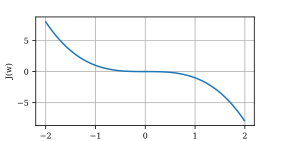
\includegraphics[scale=1]{Figures/Chapter_3/saddle_point.png}
	\end{center}
	\caption{Saddle point.} 
	\label{fig:saddle_point}
\end{figure}
%%%%%%%%%%%%%%%%%%%%%%%%%%%%%%%%%%%%%%%%%%%%%%%%%%%%%%%%%%%%%%%%%%%%%%%%%%%%%%%%
\subsection{Convolutional Neural Network} 
Convolutional Neural Networks (CNNs) are a special type of artificial neural network (ANN) that were initially developed in the 1980s by ~\textcite{Fukushima1980} who was inspired by the discoveries of Hubel and Wiesel regarding the cat's visual cortex. 
CNNs are one of the most utilised architectures in DL for image processing as they can recognise complex patterns of images by performing convolution operations.

In mathematics, a convolution is an operation performed between any two functions, as for example \(f, g:\mathbb{R}^{d} \to \mathbb{R}\) to produce at third function \((f\ast g)\) depicted in Eqn.~\ref{eqn:convolution}.
In which, we measure the overlap between \(f\) and \(g\), as one function is flipped and shifted by \(x\):
\begin{equation}
	(f\ast g)(x) = \int_{}^{} f(z)g(x-z)dz
	\label{eqn:convolution}
\end{equation}
In the case of discrete objects defined on the set \(\mathbb{Z}\) of integers, the integral operation turns into a summation of elementwise multiplied components, as depicted in Eqn.~\ref{eqn:discrete_conv}:
\begin{equation}		
	(f\ast g)(x) = \sum_{a}^{} f(a)g(i-a)
	\label{eqn:discrete_conv}
\end{equation}
For inputs with two dimensions, we have a corresponding sum with indices \((a,b)\) for \(f\) and \((i-a, j-b)\) for \(y\) respectively as depicted in Eqn.~\ref{eqn:2d_conv} that describes a cross correlation operation:
\begin{equation}
	(f\ast g)(i,j) = \sum_{a}^{}\sum_{b}^{}f(a,b)g(i-a,j-b)
	\label{eqn:2d_conv}
\end{equation}
%%%%%%%%%%%%%%%%%%%% from here
Convolution operation for image processing is essentially a cross-correlation operation also known as a sliding dot product or sliding inner-product. 
CNNs were designed to process data as tensors with different dimensions. 
For a 1D data tensor, it can represent various data forms, such as signals and sequences, in addition to sentences in various languages in translation problems.
For a 2D data tensor, it can represent an image in grayscale (one channel), further, by combining three 2D tensors a coloured 3D image is produced due to different intensities of the pixels in the (RGB) channels.
A 4D tensor represents volumetric data, such as a sequence of 3D images or a video.

A convolutional layer, has a number \( n\) of convolution kernels (filters), in  which,  each kernel has a set of weights, of a size \((w_k,h_k,d_k)\).
The kernel slides over an input image of a size \((w,h,d)\) performing a convolution operation (dot product), where \(w\) and \(h\) represent the image width and height, respectively, while \(d\) represents the depth (number of channels).
The output of the convolution operation are feature maps that are locally connected to the output of the previous layer. 
Figure~\ref{fig:convolution_3d} illustrates the convolution operation for a 3D input and the calculated output (feature map) with a new shape of \((h_{n}\times w_{n} \times d_{n})\).
%%%%%%%%%%%%%%%%%%%%%%%%%%%%%%%%%%%%%%%%%%%%%%%%%%%%%%%%%%%%%%%%%%%%%%%%%%%%%%%%
\begin{figure} [!ht]
	\begin{center}
		\centering
		\includegraphics[width=0.75\textwidth]{Figures/Chapter_3/convolution_operation_3D.png}
	\end{center}
	\caption{Convolution operation with a sliding kernel.} 
	\label{fig:convolution_3d}
\end{figure}
%%%%%%%%%%%%%%%%%%%%%%%%%%%%%%%%%%%%%%%%%%%%%%%%%%%%%%%%%%%%%%%%%%%%%%%%%%%%%%%%

Typically, the feature map size diminishes due to the convolution operation, though, the feature map can keep the same size of the input by applying some padding over the input. 
The calculations of new height and width of the output are illustrated in Eqns~\ref{new_hight} and~\ref{new_width}:
%%%%%%%%%%%%%%%%%%%%%%%%%%%%%%%%%%%%%%%%%%%%%%%%%%%%%%%%%%%%%%%%%%%%%%%%%%%%%%%
\begin{equation}
	h_{n} = \frac{h+2\times p-h_{k}}{s}+1
	\label{new_hight}
\end{equation}
%%%%%%%%%%%%%%%%%%%%%%%%%%%%%%%%%%%%%%%%%%%%%%%%%%%%%%%%%%%%%%%%%%%%%%%%%%%%%%%%
\begin{equation}
	w_{n} = \frac{w+2\times p-w_{k}}{s}+1.
	\label{new_width}
\end{equation} 
where \(h_{n}\) and \(w_{n}\) are the new height and width dimensions of the feature map respectively after applying the convolution. 
The padding \(p\) is added to the input image of a feature map to guarantee that both the input and the output have the same dimensions.
\(h_{k}\) and \(w_{k}\) represent the height and the width of the convolutional kernel, respectively.
The stride \(s\) defines how much the convolutional kernel slides each step during convolution.
The number of channels at the output feature map \((d_{n})\) equals the applied number of convolutional kernels \((n)\). 

Typically,  when we train a CNN model, its kernel weights are initialised randomly.
Accordingly, during the backpropagation process, all learnable parameters (kernels weights) are updated.
Consequently, kernels learn to detect different types of edges (vertical, horizontal, and diagonal edges), color intensities, etc.
%%%%%%%%%%%%%%%%%%%%%%%%%%%%%%%%%%%%%%%%%%%%%%%%%%%%%%%%%%%%%%%%%%%%%%%%%%%%%%%%

Commonly, a convolutional operation is followed by a non-linear activation function such as (relu, sigmoid, tanh), followed by a downsampling operation (pooling).
The idea behind pooling operation is to aggregate related features into one by reducing the spatial dimensions of the feature maps (e.g., width, height, and depth)~\cite{Lecun2015}, which reduces the computation complexity.
Figure~\ref{fig:downsampling} presents the downsampling operations that are max and average pooling, further, the pool size is \(2 \times 2\) with strides of \(2\).
The Maxpool picks the maximum value in the local pool filter in a feature map, whereas the average pool picks the average value in the local pool filter in a feature map.
%%%%%%%%%%%%%%%%%%%%%%%%%%%%%%%%%%%%%%%%%%%%%%%%%%%%%%%%%%%%%%%%%%%%%%%%%%%%%%%%
\begin{figure} [!ht]
	\begin{center}
		\centering
		\includegraphics[scale=1]{Figures/Chapter_3/downsampling.png}
	\end{center}
	\caption{Types of downsampling operations.} 
	\label{fig:downsampling}
\end{figure}
%%%%%%%%%%%%%%%%%%%%%%%%%%%%%%%%%%%%%%%%%%%%%%%%%%%%%%%%%%%%%%%%%%%%%%%%%%%%%%%%
A convolution operation, followed by a non-linear activation function, and pooling is referred to as a convolutional block.
Moreover, a convolutional block can be stacked and repeated several times. 
Finally, to pass the output from the convolutional block to the dense layer, a flattened layer is utilised to produce a 1D tensor.
Figure~\ref{fig:CNN} presents the default architecture of a CNN.
%%%%%%%%%%%%%%%%%%%%%%%%%%%%%%%%%%%%%%%%%%%%%%%%%%%%%%%%%%%%%%%%%%%%%%%%%%%%%%%%
\begin{figure} [!ht]
	\begin{center}
		\centering
		\includegraphics[width=1\textwidth]{Figures/Chapter_3/cnn.png}
	\end{center}
	\caption{Convolutional Neural Network architecture.} 
	\label{fig:CNN}
\end{figure}
%%%%%%%%%%%%%%%%%%%%%%%%%%%%%%%%%%%%%%%%%%%%%%%%%%%%%%%%%%%%%%%%%%%%%%%%%%%%%%%%

CNN became popular after the competition of the \enquote{Large Scale Visual Recognition Challenge 2012 (ILSVRC2012)}, when \textcite{Krizhevsky2012} introduced AlexNet~\cite{Krizhevsky2012}, which is a deep CNN applied on a large dataset of \(1,000,000\) images and \(1,000\) different classes.
AlexNet results were magnificent. 
The success has stimulated the progress of the development in GPUs technology and the use of the non-linear activation function Relu~\cite{Lecun2015}.
In the next years, several spectacular CNNs architectures were presented (e.g VGG-16, ResNet, Inception-v4, and others).
%%%%%%%%%%%%%%%%%%%%%%%%%%%%%%%%%%%%%%%%%%%%%%%%%%%%%%%%%%%%%%%%%%%%%%%%%%%%%%%%
\subsection{Recurrent neural networks}
\label{sec222}
Recurrent neural network (RNN) is a class of ANN that was introduced to work with time-series data (sequential data).
RNN technique can remember its data input, because of its internal memory, which makes it a powerful and promising technique in the field of DL.
Since there are temporal problems such as natural language processing, language translation, image captioning, and so on, they require to be handled sequentially.
In the traditional deep neural networks (feed-forward), the information only moves in one direction from the input layer through hidden layers to the output layers.
However, this is not the case for the RNN technique, which implies the current output of an RNN depends on the prior input sequence.
Accordingly, future events are also utilised for predicting the output of a given sequence.
Figure~\ref{fig:rnn_vs_FFNN} depicts the difference between RNN and feed-forward deep neural networks.
As shown in Fig.~\ref{fig:rrn}, for the RNN, the output of a certain layer is looped back to its input which helps in making the prediction.
However, in feed-forward networks shown in Fig.~\ref{fig:FFNN}, the inputs and outputs are independent, as there is only one direction for the data to move.
%%%%%%%%%%%%%%%%%%%%%%%%%%%%%%%%%%%%%%%%%%%%%%%%%%%%%%%%%%%%%%%%%%%%%%%%%%%%%%%%
\begin{figure}[!ht]
	\centering
	\begin{subfigure}{0.49\textwidth}		
		\centering
		\includegraphics[scale=1]{Figures/Chapter_3/recurrent_NN.png}
		\caption{} 
		\label{fig:rrn}
	\end{subfigure}
	\hfill
	\begin{subfigure}{0.49\textwidth}
		\centering
		\includegraphics[scale=1]{Figures/Chapter_3/feedforward_NN.png}
		\caption{} 
		\label{fig:FFNN}
	\end{subfigure}	
	\caption{(a) RNN v.s. (b) Feed-forward neural network.}
	\label{fig:rnn_vs_FFNN}
\end{figure}
%%%%%%%%%%%%%%%%%%%%%%%%%%%%%%%%%%%%%%%%%%%%%%%%%%%%%%%%%%%%%%%%%%%%%%%%%%%%%%%%

Figure~\ref{unrolled_rnn} presents a visualisation of an unrolled RNN, where \(x_{t}\) corresponds to the sequential timestamped input at time \(t\), \(h_{t}\) corresponds to internal state  and \(Y_{t}\) corresponds to the predicted timestamped output at time \(t\).
An unrolled RNN can be seen as a cascaded sequence of feed-forward networks.
%%%%%%%%%%%%%%%%%%%%%%%%%%%%%%%%%%%%%%%%%%%%%%%%%%%%%%%%%%%%%%%%%%%%%%%%%%%%%%%%
\begin{figure}
	\begin{center}
	\includegraphics[scale=1]{Figures/Chapter_3/unrolled_rnn.png}
	\end{center}
	\captionof{figure}{Unrolled RNN.}
	\label{unrolled_rnn}
\end{figure}
%%%%%%%%%%%%%%%%%%%%%%%%%%%%%%%%%%%%%%%%%%%%%%%%%%%%%%%%%%%%%%%%%%%%%%%%%%%%%%%%

In feed-forward neural networks, the learnable parameters (adjustable weights) are available only for the forward path of data propagation and are updated through the back-propagation algorithm.
In RNNs, there are two paths of data propagation (forward and backward). 
Hence, there are learnable weights for both directions.
Further, weights are updated using back-propagation through time (BBTT)~\cite{Werbos1990}.
BBTT depends on the number of timestamps, so it is computationally expensive when there are a high number of timestamps as BBTT performs a back-propagation algorithm on unrolled RNN.
Consequently, when implementing RNNs, issues may arise during updating the learnable weights using BBTT, which are vanishing and exploding gradients.
To overcome such issues, ~\textcite{Hochreiter1997} introduced a long short-term memory (LSTM), which is a memory extension for a regular RNN to address the problem of long-term dependencies.
Further, LSTMs handle inputs or outputs of any length, which makes LSTMs powerful for solving very complex sequential problems.
LSTM is composed of four units: an input gate, a cell state, a forget gate, and an output gate as presented in Fig.~\ref{fig:lstm}.
These gates help regulate the flow of information, which is added to or removed from the cell state. 
The hidden states in LSTM hold the short-term memory, while the cells state holds the long-term memory.
%%%%%%%%%%%%%%%%%%%%%%%%%%%%%%%%%%%%%%%%%%%%%%%%%%%%%%%%%%%%%%%%%%%%%%%%%%%%%%%%
\begin{figure}[h!]
	\begin{center}
		\includegraphics[scale=1]{Figures/Chapter_3/lstm.png}
	\end{center}
	\captionof{figure}{LSTM architecture.}
	\label{fig:lstm}
\end{figure}
%%%%%%%%%%%%%%%%%%%%%%%%%%%%%%%%%%%%%%%%%%%%%%%%%%%%%%%%%%%%%%%%%%%%%%%%%%%%%%%%

The purpose of the forget gate is to determine which information to consider and which to neglect.
The current input \(x_t\) and the previous hidden state \(h_{t-1}\) are passed through a sigmoid function which will produce values between \(0\) and \(1\).
Then the outputs of the sigmoid are multiplied with the previous cell state \(c_{t-1}\) to discard outputs equal to zero.
Equation~\ref{eqn:forget_gate} depicts the calculation at the forget gate:
%%%%%%%%%%%%%%%%%%%%%%%%%%%%%%%%%%%%%%%%%%%%%%%%%%%%%%%%%%%%%%%%%%%%%%%%%%%%%%%%
\begin{equation}
	\centering
	f_t = \sigma(W_f.[h_{t-1}, X_{t}]+ b_f),
	\label{eqn:forget_gate}
\end{equation}
%%%%%%%%%%%%%%%%%%%%%%%%%%%%%%%%%%%%%%%%%%%%%%%%%%%%%%%%%%%%%%%%%%%%%%%%%%%%%%%
where \(W\) represents the learnable weights, and \(b\) represents the bias term.

The input gate \(i_{t}\) takes the current input \(X_t\) with the previous hidden state \(h_{t-1}\) then apply the sigmoid function to get values in a range between 0 (not important) and 1 (important), then the
same current input \(X_t\), and the hidden state \(h_{t-1}\) are passed through a \(\tanh\) function at \(\tilde{C}_{t}\) that will regulate the network by transferring the values into a range between \(-1\) and \(1\).
Then, the outputs from the sigmoid and \(\tanh\) functions are multiplied point-by-point to eliminate \(0\) values.  
Equation~\ref{eq:eq2} depicts the calculation at the input gate:
\begin{equation}
	\begin{aligned}
		i_{t} &=\sigma\left(W_{i} \cdot\left[h_{t-1}, X_{t}\right]+b_{i}\right) ,
		\\
		\tilde{C}_{t} &=\tanh \left(W_{s} \cdot\left[h_{t-1}, X_{t}\right]+b_{c}\right).
	\end{aligned} \label{eq:eq2}
\end{equation}
At this point, the network has sufficient information obtained from the input and forget gates. 
Hence, the current cell state \(C_t\) is calculated by multiplying the previous cell state \(C_{t-1}\) with the output of the forget gate, then the result is added to the calculated input values as depicted in Eqn.~\ref{eq:eq3}:
\begin{equation}
	C_{t}=f_{t} * C_{t-1}+i_{t} * \tilde{C}_{t}.
	\label{eq:eq3}
\end{equation}
The output gate \(o_{t}\) computes the next hidden state \(h_{t}\) which
holds information related to the current inputs. 
Accordingly, the current input \(X_{t}\) and the previous hidden state \(h_{t-1}\) are passed through a third sigmoid function to produce values between \(0\) and \(1\).
The current cell state \(C_{t}\) is passed through a \(\tanh\) function and multiplied point-by-point with \(o_{t}\) to produce the new hidden state \(h_{t}\) which is transferred to the next timestamp.
Equation~(\ref{eq:eq4}) illustrates the calculations at the output gate:
%%%%%%%%%%%%%%%%%%%%%%%%%%%%%%%%%%%%%%%%%%%%%%%%%%%%%%%%%%%%%%%%%%%%%%%%%%%%%%%%
\begin{equation}
	\begin{aligned}
		o_{t} &=\sigma\left(W_{o}\left[h_{t-1}, X_{t}\right]+b_{o}\right),\\
		h_{t} &=o_{t} * \tanh \left(C_{t}\right).
	\end{aligned}
	\label{eq:eq4}
\end{equation} 
%%%%%%%%%%%%%%%%%%%%%%%%%%%%%%%%%%%%%%%%%%%%%%%%%%%%%%%%%%%%%%%%%%%%%%%%%%%%%%%%

Recently, LSTMs have been widely used for large-scale learning of language translation models, speech recognition systems, chatbots, forecasting stock markets, text data analysis, and many more~\cite{graves2014towards, cho2014properties}.
However, LSTMs are inefficient regarding capturing spatial information by themselves when the time series inputs are consecutive images.
Accordingly, the ConvLSTM layer, which is a combination of CNN and LSTM unit was introduced by Shi et al.~\cite{xingjian2015convolutional} to solve such a problem.
For ConvLSTM, the convolution operations are applied both at the input-to-state transition and at the state-to-state transitions.
ConvLSTM shown in Fig.~\ref{fig:ConvLSTM} is a variation of the LSTM cell as it performs a convolution operation within the LSTM cell.
%%%%%%%%%%%%%%%%%%%%%%%%%%%%%%%%%%%%%%%%%%%%%%%%%%%%%%%%%%%%%%%%%%%%%%%%%%%%%%%%
\begin{figure}[h!]
	\begin{center}
		\includegraphics[scale=1]{Figures/Chapter_3/convlstm_image.png}
	\end{center}
	\captionof{figure}{ConvLSTM architecture.}
	\label{fig:ConvLSTM}
\end{figure}
%%%%%%%%%%%%%%%%%%%%%%%%%%%%%%%%%%%%%%%%%%%%%%%%%%%%%%%%%%%%%%%%%%%%%%%%%%%%%%%%
ConvLSTM is a combination of a convolution operation and an LSTM cell.
Thus, ConvLSTM can capture the time-correlated and spatial features in a series of consecutive images. 
Equation~(\ref{eq:eq5}) depicts the ConvLSTM operations as the inputs \(X_1, \dots, X_t\), hidden states \(h_1, \dots, h_t\), cell states \(C_1, \dots, C_t\) and input, forget and output gates are represented as \(i_t, f_t\), and \(o_t\), respectively:
\begin{equation}
	\begin{aligned}
		i_{t} &=\sigma\left(W_{x i} * X_{t}+W_{h i} * h_{t-1}+W_{c i} \odot C_{t-1}+b_{i}\right) 
		\\
		f_{t} &=\sigma\left(W_{x f} * X_{t}+W_{h f} * h_{t-1}+W_{c f} \odot C_{t-1}+b_{f}\right) \\
		C_{t} &=f_{t} \odot C_{t-1}+i_{t} \odot \tanh \left(W_{x c} * X_{t}+W_{h c} * h_{t-1}+b_{c}\right) 
		\\
		o_{t} &=\sigma\left(W_{x o} * X_{t}+W_{h o} * h_{t-1}+W_{c o} \odot C_{t}+b_{o}\right) \\
		h_{t} &=o_{t} \odot \tanh \left(C_{t}\right)
	\end{aligned}
	\label{eq:eq5}
\end{equation}
where \(*\) indicates the convolution operation, and \(\odot\) represents the 
Hadamard product. 
Recently, ConvLSTM has become very popular and is increasingly being used in 
more and more image processing applications.
\section{Data-driven based SHM/NDT Techniques: Related work}
\label{sec33}
%%%%%%%%%%%%%%%%%%%%%%%%%%%%%%%%%%%%%%%%%%%%%%%%%%%%%%%%%%%%%%%%%%%%%%%%%%%%%%%%
The importance of SHM systems originates from their ability to monitor the condition of structures in real-time.
SHM systems can be developed using data-driven methods, which require a huge amount of data that are captured by monitoring the status of a structure.

The process of extracting features from structures in conventional techniques needs a lot of time and experts in the field.
Therefore, introducing machine learning methods to the feature extraction process became necessary.
Hence, deep learning methods can generalise and learn new features by themselves, which improves their functionality in damage estimation.

DL approach makes it possible to use registered data in their raw form without any need to perform feature extraction.
Hence, such an approach has an end-to-end structure that automatically learns and discovers the hidden features in a high dimensional input data~\cite{LeCun, Networks}.
Figure~\ref{fig:ML_vs_DL} illustrates the main differences between the conventional ML-based SHM and DL-based SHM approaches.

\begin{figure}[!ht]
	\centering
	\begin{subfigure}{1\textwidth}		
		\centering
		\includegraphics[width=1\textwidth]{Figures/Chapter_3/conventional_ML.png}
		\caption{} 
		\label{fig:ML_conventional}
	\end{subfigure}
	\\
	\begin{subfigure}{1\textwidth}
		\centering
		\includegraphics[width=1\textwidth]{Figures/Chapter_3/DL_approach.png}
		\caption{} 
		\label{fig:DL_approach}
	\end{subfigure}	
	\caption{(a) Conventional ML based SHM vs. (b) DL based SHM.}
	\label{fig:ML_vs_DL}
\end{figure}
%%%%%%%%%%%%%%%%%%%%%%%%%%%%%%%%%%%%%%%%%%%%%%%%%%%%%%%%%%%%%%%%%%%%%%%%%%%%%%%%
\textcite{Worden2007} have proposed several axioms related to SHM systems implemented using machine learning methods. 
According to them, damage detection can be perform\-ed in unsupervised learning.
However, recognising the damage type and how significant it is can not be performed without supervised learning. 
Moreover, the feature extraction process is essential for damage detection, and it can be performed by analysing and processing the signals captured by the sensors (e.g. PZT actuators), and then converting them to damage information.
Therefore, introducing machine learning methods to the feature extraction process became necessary.
Hence, machine learning methods can generalise and learn new features by themselves, which improves their functionality in damage estimation.

\subsection{Machine learning based SHM/NDT}
In recent years data-driven methods based on machine learning have increased in a significant way. 
In the following, I will present some methods for damage detection and estimation based on machine learning techniques.

%%%%%%%%%%%%%%%%%%%%%%%%%%%%PZT + SVM
\textcite{Das2010} presented a method for estimating several types of defects (delamination, saw cut, notches, and drilled holes) in composite material. 
For this purpose, a collection of PZT transducers were attached to the surface of the structure to generate and register Lamb waves propagation. 
Accordingly, a time-frequency domain was utilised to extract features related to defects from the registered response. 
Those extracted features were fed to one-class SVM, which performs classification and damage estimation. 
%%%%%%%%%%%%%%%%%%%%%%%%%%%% PZT + SVM

Moreover, \textcite{Dib2018} proposed a novelty classifier based on one-class SVM for detecting damage. 
The method was conducted by extracting data from damage impact on a glass-fibre composite plate and then evaluating the performance of the classifier. 
To extract the necessary features from the propagated wave the registered signal was segmented into L time bins, and the Fourier transform was applied to each time bin.
Accordingly, the features vector was constructed from the signal phase and the amplitude for each segmented time bin.
%%%%%%%%%%%%%%%%%%%%%%%%%%%%%%%%% PZT + PCA+ KNN + SVM

\textcite{Vitola2016} developed a damage detection and classification methodology that was examined on aluminium plates.
An array of PZT transducers was placed on the plate surface to sense wave propagation in the structure.
The methodology is based on the use of principal component analysis (PCA) and machine learning techniques for recognising patterns.
PCA means analysing a large amount of information by finding the principal components.
However, the PCA method is not invariant to scaling, thus, data must be normalized~\cite{Tibaduiza2016}.
Next, normalised data is fed to several machine learning models for training.
For this purpose, several classification algorithms were applied, decision trees, KNN and SVM.
However, only a few of these models presented good outputs in damage detection.

%%%%%%%%%%%%%%%%%%%%%%%%%%% KNN
\textcite{Godin2004} applied Acoustic Emission signals (AE) in their approach, which happen due to a sudden release of stored energy when damage occurs.
AE signals contain important information about the discriminative features 
for the damage type such as fibre breakage, de-cohesion of the interface, or a crack in the matrix in composite materials.
Authors in this work presented supervised and unsupervised classifiers to recognise different damage patterns through grouping AE signals from the tensile tests of unidirectional glass/polyester composite into several different classes. 
For clustering AE signals, a K-means algorithm was used. 
AE signals were clustered based on several metrics such as the AE signal duration, amplitude, rise time, and the number of counts to the peak.
Accordingly, the clustered labelled data is fed into a KNN supervised classifier.
A trained classifier can classify new coming data accordingly.
Regarding the unsupervised classification, the Kohonen classifier was utilised~\cite{58325}, which is a self-organising map (SOM) which is a neural network consisting of neurons as processing units. 

%%%%%%%%%%%%%%%%%%%%%%%%%%% 

\textcite{Nazarko2020} monitored the axial bolt forces using elastic wave propagation signals.
Six-bolt flange connections were put through a series of static tensile tests in the lab. 
For the accurate measurement of axial force, some bolts were equipped with washer load cells.
Additionally, a few bolts were equipped with piezoelectric transducers (actuator and sensor operating in a pitch-catch arrangement) to capture the elastic wave signals.
The outcomes of the ultrasonic testing were then integrated with the artificial neural network (ANN) for both signal compression and as a tool for user interface. 
The outcomes demonstrated that ANNs could predict the axial forces in bolts with a reasonable amount of accuracy. 
Significant potential exists for actual NDT inspections, according to the suggested method~\cite{Nazarko2020}. 

%%%%%%%%%%%%%%%%%%%%%%%%%%% KNN
\textcite{Pashmforoush2014} proposed a technique to classify damage to various lay-up configurations in glass/polyester composites.
For this purpose, the K-means algorithm with the genetic algorithm was utilised. 
PCA was used to reduce the data dimensionali\-ty.
Next, a combination of the K-means algorithm with the genetic algorithm is used for clustering the data. 
The reason for applying the genetic algorithm is to find the optimal number of cluster centres for the KNN algorithm.
Parameters of the AE signals such as peak amplitude, frequency, rise time, energy, and duration were estimated for each cluster and utilised as discriminative features. 
AE signal frequency was found to be a good feature for discrimination. Accordingly, AE signals with the highest frequency were corresponding to fibre breakage, AE signals with the lowest frequency were corresponding to matrix cracking, and the frequencies range in-between were corresponding to the debonding defect. 

%%%%%%%%%%%%%%%%%%%%%%%%%%%%%%%%%%%%%%%%%%%%%%%%%%%%%%%%%%%%%%%%
\textcite{Nazarko2016} investigated the potential of utilising artificially deteriorated signals of Lamb waves in training a novelty detection (ND) system for early damage detection.
To train auto-associative neural networks, the authors used principal components that were generated from signals that were measured experimentally.
The measurements of Lamb waves in the investigated specimens made of aluminium and glass fibre reinforced polymer serve as an excellent illustration of how the ND algorithm accurately handles both simple and complex signals.
It was also noted that the proposed ND method maintained its sensitivity and robustness when it used raw signals with a relatively low sampling rate, on a relatively narrow time window, and further noised signals.
%%%%%%%%%%%%%%%%%%%%%%%%%%%% PZT + ConvNet
%\textcite{Sammons2016} utilised X-ray computed tomography for estimating the delaminations in a CFRP. For this purpose, they utilised the Convolutional Network (ConvNet ) for performing image segmentation of the defected input images to estimate the delaminations. There ConvNet was capable of identifying  and quantifying small delaminations. 
%Unfortunately, the ConvNet could not recognise delaminations with large sizes.
%%%%%%%%%%%%%%%%%%%%%%%%%%%% PZT + ConvNet
%
%Moreover, \textcite{Chetwynd2008} have investigated curved carbon fibre composite panel for damage localisation. 
%Accordingly, stiffeners were used during the experiments to represent real-life damage. 
%For this purpose, authors attached a combination of PZT transducers on the panel used to generate and receive Lamb waves that propagate through the structure. 
%During their propagation through the structure, Lamb waves encounter defects, which affects their propagation response. 
%The collected response was transformed into a novel scaler index using outlier analysis~\cite{Beniger1980}, which was then fed to MLP. 
%The MLP used for classification and regression applications of damage detection. 
%Classification operation is responsible for predicting whether there is damage or not in a specific location. 
%Where the regression operation is responsible for the exact estimation of the damage location.
%%%%%%%%%%%%%%%%%%%%%%%%%%% Ful wavefield +ConvNets
%% SECTION HEADER ////////////////////////////////////////////////////////////////////////////////
\subsection{Deep learning based SHM/NDT}

Deep learning techniques have widely been utilised for the inspection and maintenance of civil infrastructure and have shown very promising results \cite{Cha2017b, Lin2017, liu2019computer, Beckman2019, Choi2020, Sonski2020a, Sonski2020, Sonski2019}. 

Besides the widespread applications of deep learning for SHM/NDT in civil engineering, deep learning is still less investigated for the purpose of damage detection based on guided waves in composite materials.

Guided waves approaches are widely utilised in SHM/NDT due to the fact it can detect very small damage sizes~\cite{Guemes2020}. 
Damage detection and localisation approaches using guided waves are based on the measurements of the PZT sensors, whether bonded or embedded into the investigated structure. 
PZT sensor(s) are responsible for the excitation of the structure by a short ultrasonic pulse (usually, the used frequency is in the range of hundreds of kHz) that propagates through an investigated structure such as plates or pipes as an elastic wave.
The registered signals (baseline) are stored and compared with other registered signals acquired through the lifetime of the investigated structure.
Damage detection using the baseline subtraction approach for guided waves is based on subtracting damage-free registered measurements from the newly registered measurements to obtain the new changes that occurred to the structure.
These changes are considered as damage information.
The baseline approach is effective in controlled environments where the variations of the operational/environments (i.e. considerations of multiple sensing modalities, uncertainty in material properties, bounding conditions, etc.) are negligible~\cite{Yuan2020}.  
Such variations can alter registered data leading to false alarms.
The effect of such variations can be reduced through physics-based modeling, which can simulate an undamaged scenario (baseline) for the wave propagation through the investigated structure.
Then, the simulated baseline can be used in the subtraction for damage detection.
However, in real-world structures, it is difficult to adjust the parameters of the model to match the experimental registered data.
Accordingly, data-driven techniques based on ML and DL approaches can be the solution and deliver robust models for many real-life variations.

In the following, methods for damage size estimation based on machine learning and deep learning techniques are presented, which are targeted in the field of SHM/NDT.

%\textcite{islam1994damage} presented one of the earliest research studies for assessing delamination location and size in composite structures using deep learning techniques.
%They trained a neural network model using frequencies from modal analysis data for the first five modes.
%Data were obtained using piezoceramic sensors in both damaged and undamaged composite beams.
%In the following, several approaches utilising guided waves for SHM/NDT based on data-driven techniques for damage detection and localisation are presented.

\textcite{Melville1949} proposed a CNN model for the prediction of damage state in thin metal plates to overcome the issue of inaccurate representation of guided wave propagation when applying conventional approaches. 
The model utilizes the full wavefie\-ld scans of thin plates (aluminium).
Moreover, the acquired raw data used for training the model was divided into undamaged and damaged states equally.
The model achieved higher accuracy regarding damage detection equal \(99.98\%\) when compared to SVM which achieved \(62\%\).

\textcite{Sammons2016} proposed a CNN model based on X-ray computed tomography for delamination estimation in a composite structure.
Furthermore, image segmentation was applied to the input images to identify the damage.
However, the model was only able to identify small delaminations.

Moreover,~\textcite{Chetwynd2008} presented a multi-layer perceptron (MLP) network for damage detection in curved composite panels, in which, stiffeners were added to represent the damage.
The Authors in this work investigated the propagation of Lamb waves through the panel in which they were generated and registered by a PZT array.
Furthermore, for each Lamb wave response, a novelty index was obtained.
The index value is compared to some threshold value, in which if the index value exceeds the threshold it implies that there is damage to the structure.
Accordingly, the MLP network was fed by obtained novelty indexes, and performed two operations: classification and regression.
The classification network was designed to define three convex regions of the panel and then to determine whether the panel is damaged or not.
On the other hand, the regression network is capable of estimating the exact location of the damage

Furthermore,~\textcite{DeFenza2015} proposed an artificial neural network (ANN) model for damage detection in plates made of aluminium alloys and composite utilising Lamb waves.
Response data of wave propagation were used to calculate damage indexes which were fed into the model as an input.
Accordingly, the model performs automatic feature extraction in conjunction with the probability ellipse-based method. 
The ANN model and probability ellipse (PE) method were applied to identify the damage location.
The results from the ANN model and the PE presents how it is useful to apply damage indexes as a baseline for such methods to evaluate damage in aluminium and composite structures. 
Ewald et al.~\cite{Ewald2019} presented a CNN model called (DeepSHM) for signal classification using Lamb waves.
Furthermore, the model provides an end-to-end approach for SHM by utilising response signals captured by sensors.
Moreover, response signals were preprocessed by wavelet transform to get the wavelet coefficient matrix (WCM).
Further, the CNN model was trained with the WCM to obtain neural weights.

Full wavefield scanning using SLDV is time-consuming, however, simply reducing the number of scanning points will result in low-quality images. 
\textcite{esfandabadideep} proposed a compressive Sensing technique using ConvNets to enhance the resolution for images captured by SLDV while decreasing the number of measurement scan points down to \(10\%\) of the number of the full gird scanning points. 
Although, the proposed technique enhanced the image resolution, however, there is a side effect, which resembles the fact when enhancing the resolution, the most affected region is the damaged area. 
Accordingly, the damage features will be altered.
On the other hand, this may be an indication of the location of the damage.

Furthermore,~\textcite{Melville2018} proposed a technique for damage detection in thin metal plates (aluminum and steel), using full wavefield data scanned by SLDV. 
Using this data to train a deep neural network of 4 hidden layers including 2 convolutional layers for features extraction and 2 fully connected layers. 
The developed model shown good results when compared with traditional machine learning SVM.
Moreover,~\textcite{Melville2017} introduced a method for detecting damage in structures based on the k-means algorithm. 
The method is known as~\enquote{dictionary learning} which uses full wavefield data collected from thin metal plates. 
The method was applied to structures with different material types and thicknesses that were not used during training to prove how well the model in damage detection in various conditions. 
However, their work was not implemented for a further step, which is damage localization and classification.

%\textcite{Ijjeh2021} presented a fully convolutional network (FCN)  for damage identification in composite plates base on a supervised learning approach.
%Furthermore, the authors utilised a full wavefield of Lamb waves propagation, which was numerically generated resembling measurements acquired by scanning laser Doppler vibrometer (SLDV).
%The model performs a pixel-wise segmentation that is able to identify the delamination which results in damaged and undamaged classes.
%Moreover, the model results were validated through a comparison with a conventional wavefield signal processing method i.e. adaptive wavenumber filtering~\cite{Radzienski2019,Kudela2018}.
%The proposed model achieved an accuracy of \(93.3\%\) in damage detection on numerical data compared to  \(64.8\%\) with the conventional method.
%Furthermore, the proposed model was verified on experimental data and it proved its ability for generalisation.
%%%%%%%%%%%%%%%%%%%%%%%%%%%%%%%%%%%%%%%%%%%%%%%%%%%%%%%%%%%%%%%%%%%%%%%%%%%%%%%%%%%%%%%%%%%%%%%%%%%%%%%%%%%%%%%%%%%%%%%%%%%%%%%%%%%%%%%%%%%%%%%%%%%%%%%%%%%%%%%%
%\subsection{Vibration based SHM though DL}
%\label{sec24}
%The vibration-based approach for damage assessment using ML techniques has been investigated thoroughly  for several SHM applications.
%Furthermore, introducing DL techniques for data-driven SHM applications has presented new scopes for investigating large scale structures and enhanced the process of data acquisition and processing of large datasets acquired by sensors of different types~\cite{Carden2004,Sohn1996}.
%Generally, the conventional approach for damage localisation requires prior knowledge of the approximate damage locations~\cite{Xu2018,Dorafshan2016}. 
%Therefore, the identification process regarding candidates for the damaged locations is complex and can consume plenty of time.
%Damage locations identification under the vibrational approach is based on the fact that the damage cause changes in the vibration characteristics such as modal shapes, frequencies, and damping~\cite{Doebling1998},
%which can be utilised in the identification of damaged locations from the registered data response of a structure.
%A vibration-based approach can be categorised into two classes:
%model-based (parametric) and non-model-based or (non-parametric).
%Parametric methods require computational models and associated assumptions about the investigated structure.
%In general parametric methods can achieve good accuracy, however, there is no guarantee regarding the availability of accurate information about the structural system in the real-world~\cite{Azimi2020}. 
%As a result, the non-parametric methods arise due to the challenges in developing robust computational models. 
%With non-parametric methods, there are no prior assumptions about the structural system.
%
%In the following, several vibration-based for SHM using DL techniques are presented.
%Authors in~\cite{Abdeljaber2017} introduced a damage identification approach based on output-only response data.
%In which, various damage cases (loose bolt) were investigated, accordingly training data were generated based on the acceleration response.
%Authors in this approach have trained several CNNs separately regarding each damage case, and accordingly, the probability of damage (PoD) was determined.
%By investigating scenarios of undamaged, single damage and multiple damage cases, they obtained \(0.54\%\) average error for specifically identified cases.
%
%Authors in~\cite{Lin2017} introduced a new approach to structural damage detection using CNN.
%Moreover, the authors have developed a numerical model of simply supported Euler Bernoulli beam.
%The detection model was designed to learn features and to identify damaged locations, moreover, it led to excellent results regarding the accuracy of damaged locations on the noise-free and noisy dataset.
%Wang and Cha in~\cite{Cha2018} proposed an unsupervised CNN model, that is able to extract the feature representations from the unlabelled data.
%The authors in their model used raw acceleration signals (sensitive to the damage presence) that were acquired from an intact lab-scale steel bridge.
%Then, the acquired response vector was normalised followed by applying the continuous wavelet transform (CWT) and fast Fourier transform (FFT).
%The output was then fed into a CNN auto-encoder,
%Accordingly, the extracted damage features were fed into one-class (OC) SVMs as novelty detectors corresponding to the sensors.
%Consequently, the approximation of damage location (loose-bolt) was estimated based on the locations of the sensors with the highest novelty rates.
%
%Motivated by human vision and thinking, authors in~\cite{Cha2018} presented a computer vision and deep-learning framework for anomaly detection.
%The proposed approach consists of two steps.
%In the first step, data conversion by data visualisation is carried out, in which it mimics human vision and thinking.
%In data visualisation,  the registered data response of acceleration is transformed into images plotted in gray-scale. 
%In the second step, the training dataset is labeled manually, then fed into deep convolutional neural networks (DCNNs).
%The proposed technique was tested on one-year data and achieved a global accuracy of \(87,0\%\) and it could be used for real-time SHM.
%Moreover, Tang et al. in~\cite{Tang2019} presented a DL technique for data anomaly detection which can be considered as an improved technique to the previous work in~\cite{Cha2018}.
%Initially, the raw time series measured data are split into segments, and data in the time and frequency domain are visualised. 
%Images related to each section are stacked as a single dual-channel (red and green).
%Then, the training dataset is fed into a CNN that learns how to perform data anomaly classification.
%The main difference between the previous approach and this approach was in using imbalanced data in which the number of samples of different classes was unequal, however, in this approach the used data were balanced.
%Finally, the comparison shows that this approach outperformed the previous one and achieved higher accuracy for all data anomaly patterns.
%
%Authors in~\cite{Wu2019} presented a study of the deep CNN method in estimating the dynamic response of a linear single-degree-of-freedom (SDOF) system, a nonlinear SDOF, and a multidegree of freedom (MDOF) streel frame.
%In some cases, the convolutional kernel can approximate the numerical integration operator, and the convolutional layer can be interpreted as a dominant frequency extraction operator.
%Moreover, different cases of noise-contaminated signals were investigated. 
%Additionally, MLP method was used as a reference to the proposed CNN approach.
%A comparison between the results obtained by the MLP and CNN shows that the CNN approach is more accurate and robust against noisy input data.
%
%Authors in ~\cite{Oh2019}  presented a study of the CNN technique for SHM application for response estimation of tall buildings under wind excitation.
%The proposed CNN model was trained on measured structural response data which take wind data measured as inputs in order to predict strains in future wind loads.
%In order to measure the performance of the proposed technique, it was verified with unseen data never used at the training phase and it was able to accurately estimate the maximum and minimum strains.
%Authors in~\cite{Li2020} proposed a CNN model for damage detection of a bridge structure.
%Moreover, the authors compared the performance of the CNN model with other techniques such as random forest, SVM, KNN, and decision tree, and the results showed that the accuracy was enhanced by at least \(15\%\).
%
%Since the acceleration response signal is highly prone to noise~\cite{Azimi2020}, researchers begin utilising other types of sensor data or use alternative features.  
%Li et al. in ~\cite{Li2020a} investigated damage in bridge structure accordingly, proposed a supervised learning technique based on the CNN model.
%Dataset was acquired by deflection of a scaled-down model bridge by a fibre-optic gyroscope.
%Then, the dataset was fed into a 1D-CNN model to classify three states of damage and an intact class (benchmark/damage-free).
%To investigate the performance of the proposed model, a cross-validation technique was applied. 
%It showed that the accuracy of the CNN model increased by at least \(15.3\%\) over other conventional methods such as SVM, KNN, decision trees, and random forests.
%Authors in \cite{Lopez-Pacheco2020} introduced a novel frequency-domain convolutional neural network (FDCNN) for damage detection based on Bouc-Wen hysteric model~\cite{Ismail2009}.  
%In the FDCNN method utilises only acceleration measurements for damage diagnosis, that are sensitive to environmental noise.
%Moreover, FDCNN reduces the computational time during the learning process, which increase noise robustness.
%The FDCNN introduced the spectral pooling operator responsible for attenuating the noise in measurements.
%The proposed method was validated through comparing it with different CNN model. 
%The performance of the proposed method was higher regarding damage identification in building structures.
%
%Finally, with smart monitoring as a target, authors in~\cite{Hung2020}  proposed a hybrid deep learning model for damage detection for SHM.
%The proposed model can deal with different damage levels and accurately detect damage by combining 1D-CNN and Long-Short Term Memory (LSTM) into a single end-to-end model fed by the raw time-series, and as a result, avoiding signal preprocessing step.
%Moreover, the proposed model verified that with low noise levels,  accurate damage detection can be achieved.
\section{Summary}
\label{sec34}
Moreover, author presented in this chapter several techniques that had studied and examined guided Lamb waves in composite materials to detect and localise the damage using signal processing techniques. 
Consequently, author concluded that those traditional techniques are complex and involve a huge numerical analysis and signal processing. Which concluded that the damage features are difficult to be extracted manually. 
Thus, new approaches that involve Machine and Deep Learning techniques are utilised are presented in this chapter. 
As a result, the process of damage features extracting became more convenient and easier since the machine is responsible for learning the new features and accordingly  detect and localise the damage. 
In consequence, it is concluded that the advantage of this approach is the improvement of feature damage extracting procedure.

Furthermore, problems with conventional damage detection techniques for SHM and the importance of the artificial intelligence approach were discussed.
Furthermore, in the second section of the chapter, the author introduced the ML approach in the SHM field.
Moreover, several techniques for feature extraction such as PCA, MSD, and GMMs were described. 
Further, several classification models such as SVM, KNN, and decision trees were introduced.
In the third section, DL approach was presented, in which techniques such as CNN  and RNN were presented.
Finally, several deep learning techniques for damage detection used regarding the SHM field based on guided waves and vibration approaches were presented.
%\input{Chapters/Chapter3/sect35}
%\input{Chapters/Chapter3/sect36}
	%% CHAPTER HEADER /////////////////////////////////////////////////////////////////////////////////////
\chapter[Methodology]{Methodology}
\label{ch4}

%% CHAPTER INTRODUCTION ///////////////////////////////////////////////////////////////////////////////

We need to illustrate the dataset and what does it resembles thoroughly.
Then talk about all models from bounding boxes, RMS input models and full wave field frames models with extreme explanation. Lots of tables and figures

%% INCLUDE SECTIONS ///////////////////////////////////////////////////////////////////////////////////

%% SECTION HEADER /////////////////////////////////////////////////////////////////////////////////////
\section{Synthetic data acquisition}
\label{sec41}
%%%%%%%%%%%%%%%%%%%%%%%%%%%%%%%%%%%%%%%%%%%%%%%%%%%%%
The crucial part in our work was in synthetically generating a dataset of a full wavefield of propagating of Lamb waves in a plate made of CFRP.
In which we
In this work, we have generated a large dataset of \(475\) cases of a full wavefield of propagating Lamb waves in a plate made of carbon fibre-reinforced plastic (CFRP).
The in-house code of the time-domain spectral element method was used for simulation of Lamb wave interaction with delamination~\cite{Kudela2020}.
It should be added that despite the utilisation of the parallel code of the spectral element method which was run on the Tesla K20X GPU card, the computation of the dataset (consisting of 475 cases) took about 3 months.
For each case, single delamination was modelled by using the method of splitting nodes between appropriate spectral elements. 
It was assumed that the composite laminate is made of eight layers of a total thickness of 3.9 mm.
The delamination was modelled between the third and fourth layer (see Fig.~\ref{fig:plate_setup} for details).
It should be noted that Fig.~\ref{fig:plate_setup} shows an exaggerated cross-section through the delamination. 
Zero-volume delamination was assumed in the model. 
Delamination spatial location was selected randomly so that the interaction of guided waves with delamination is different for each case.
It includes cases when delamination is located at the edge of the plate which is the most difficult to identify by signal processing methods.
Additionally, the size of the delamination of elliptic shape was randomly simulated by selecting the size of ellipse minor and major axis.
Also, the angle between the delamination major axis and the horizontal axis was randomly selected.
In summary the following random factors were simulated in each case:
\begin{itemize}
	\item delamination geometrical size	(ellipse minor and major axis randomly selected from the interval \(\left[10 \, \textrm{mm}, 40\, \textrm{mm}\right]\)),
	\item delamination angle (randomly selected from the interval \( \left[ 0^{\circ}, 180^{\circ} \right]\)),
	\item coordinates of the centre of delamination (randomly selected from the interval \(\left[0\, \textrm{mm}, 250\, \textrm{mm} -\delta \right]\) and \( \left[250\, \textrm{mm}+\delta, 500\, \textrm{mm} \right] \), where \(\delta = 10\, \textrm{mm}\)).
\end{itemize}
It resulted in random spatial placement of delaminations. The plate with overlayed 475 delamination cases is shown in Fig.~\ref{fig:random_delam}.
\begin{figure}
	\centering
	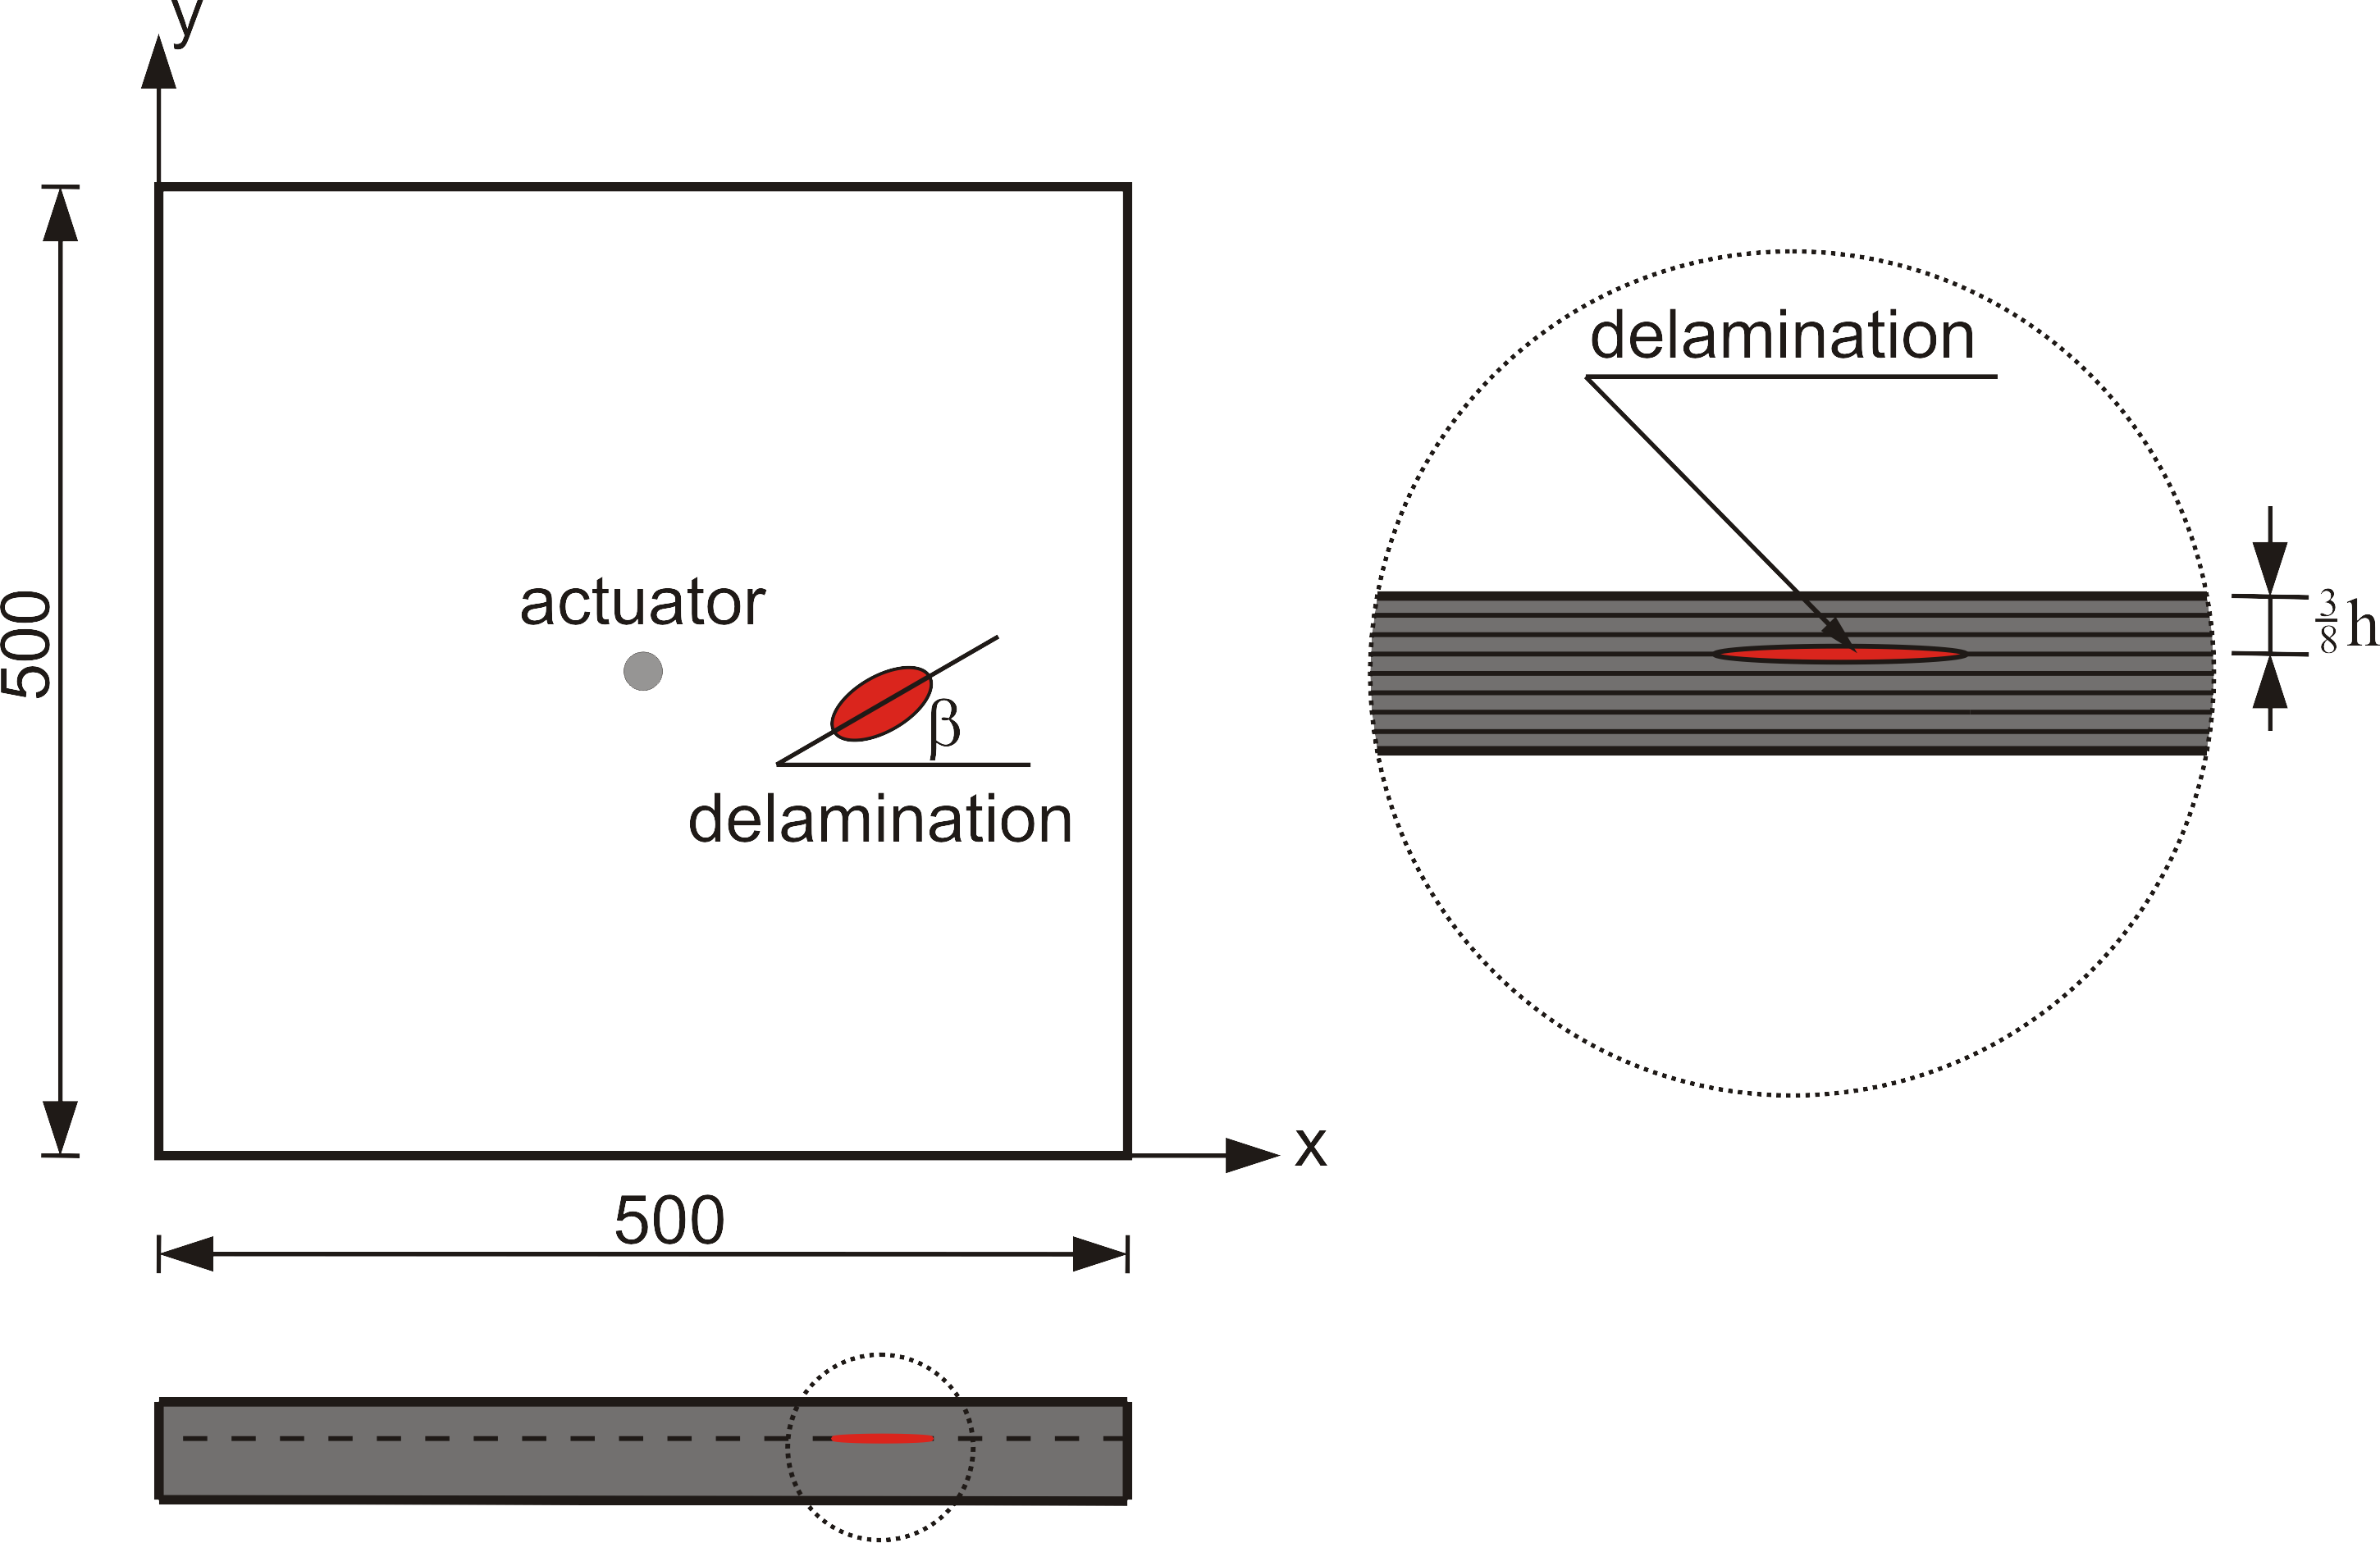
\includegraphics[scale=0.8]{Figures/Chapter_3/plate_delam_arrangement_MSSP.PNG}
	\caption{Setup for computing Lamb wave interactions with delamination.}
	\label{fig:plate_setup}
\end{figure}	
\begin{figure}
	\centering
	\includegraphics[scale=1]{Figures/Chapter_3/dataset2_labels_ellipses.png}
	\caption{The plate with 475 cases of random delaminations.}
	\label{fig:random_delam}
\end{figure}

Guided waves were excited at the plate centre by applying equivalent piezoelectric forces.
The excitation signal had a form of sinusoid modulated by Hann window. 
It was assumed that the carrier frequency is 50 kHz and the modulation frequency is 10 kHz.
A relatively low carrier frequency allowed for lower mesh density and significant computation time reduction in comparison to simulations of higher frequencies.
Additionally, the excitation signal was selected so that interaction of generated A0 Lamb wave mode with the smallest delamination can be still used as a feature for damage identification.

The output from the top and bottom surfaces of the plate in the form of particle velocities at the nodes of spectral elements were interpolated on the uniform grid of 500\(\times\)500 points by using shape functions of elements (see~\cite{Kudela2020} for more details).
It essentially resembles measurements acquired by SLDV in the transverse direction (perpendicular to the plate surface).
An example of the simulated full wavefield data on the top and bottom surfaces is presented in Fig.~\ref{fig:wavefield}.
It should be noted that stronger wave entrapment at delamination can be observed for the case of the wavefield at the top surface.
It is because the delamination within cross-section is located closer to the top surface.
It makes it easier to detect delamination by processing wavefield at the top surface.
It is better visible if the root mean square (RMS) according to Eq.~(\ref{eq:rms}) is applied to the wavefield.
The result of this operation is presented in Fig.~\ref{fig:rms}.
Based on the image analysis, the shape of the delamination can be easier to discern for the top case.
However, the methodology presented in this paper was applied to the more difficult case i.e. wavefield registered at the bottom surface of the plate.

%The dataset consisting of RMS images which were used in this research paper is available online~\cite{Kudela2020d}.

\begin{figure} [h!]
	\centering
	\begin{subfigure}[b]{0.32\textwidth}
		\centering
		\includegraphics[scale=1]{Figures/Chapter_3/96_flat_shell_Vz_1_500x500top.png}
		\caption{\(t=0.141\) ms}
		\label{fig:frame96top}
	\end{subfigure}
	\hfill
	\begin{subfigure}[b]{0.32\textwidth}
		\centering
		\includegraphics[scale=1]{Figures/Chapter_3/128_flat_shell_Vz_1_500x500top.png}
		\caption{\(t=0.188\) ms}
		\label{fig:frame128top}
	\end{subfigure}
	\hfill
	\begin{subfigure}[b]{0.32\textwidth}
		\centering
		\includegraphics[scale=1]{Figures/Chapter_3/164_flat_shell_Vz_1_500x500top.png}
		\caption{\(t=0.240\) ms}
		\label{fig:frame164top}
	\end{subfigure}	
	\hfill
	\begin{subfigure}[b]{0.32\textwidth}
		\centering
		\includegraphics[scale=1]{Figures/Chapter_3/96_flat_shell_Vz_1_500x500bottom.png}
		\caption{\(t=0.141\) ms}
		\label{fig:frame96bottom}
	\end{subfigure}
	\hfill
	\begin{subfigure}[b]{0.32\textwidth}
		\centering
		\includegraphics[scale=1]{Figures/Chapter_3/128_flat_shell_Vz_1_500x500bottom.png}
		\caption{\(t=0.188\) ms}
		\label{fig:frame128bottom}
	\end{subfigure}
	\hfill
	\begin{subfigure}[b]{0.32\textwidth}
		\centering
		\includegraphics[scale=1]{Figures/Chapter_3/164_flat_shell_Vz_1_500x500bottom.png}
		\caption{\(t=0.240\) ms}
		\label{fig:frame164bottom}
	\end{subfigure}
	
	\caption{Full wavefield at the top surface (a)--(c) and the bottom surface (d)--(f), respectively, at selected time instances showing the interaction of guided waves with delamination.}
	\label{fig:wavefield}
\end{figure} 

\begin{figure} [h!]
	\centering
	\begin{subfigure}[b]{0.47\textwidth}
		\centering
		\includegraphics[scale=1]{Figures/Chapter_3/RMS_flat_shell_Vz_1_500x500top.png}
		\caption{top}
		\label{fig:rmstop}
	\end{subfigure}
	\hfill
	\begin{subfigure}[b]{0.47\textwidth}
		\centering
		\includegraphics[scale=1]{Figures/Chapter_3/RMS_flat_shell_Vz_1_500x500bottom.png}
		\caption{bottom}
		\label{fig:rmsbottom}
	\end{subfigure}
	\caption{RMS of the full wavefield from the top surface of the plate (a) and the bottom surface of the plate (b).}
	\label{fig:rms}
\end{figure} 

%% SECTION HEADER ////////////////////////////////////////////////////////////////////////////////
\section{Delamination detection using fully connected CNN classifier}
\label{sec42}

In this section, I present my initial attempt to solve the problem of delamination detection in CFRP materials by utilising CNN models for classification purposes.

The bounding box method was used for the classification of the location of the delamination with the input as RMS (Fig.~\ref{fig:RMS_14}) and the binary representation of the delamination shape as ground truth (label shown in Fig.~\ref{fig:label_14}).
%%%%%%%%%%%%%%%%%%%%%%%%%%%%%%%%%%%%%%%%%%%%%%%%%%%%%%%%%%%%%%%%%%%%%%%%%%%%%%%%
\begin{figure} [!ht]
	\centering
	\begin{subfigure}[b]{0.47\textwidth}
		\centering
		\includegraphics[width=5cm]{Figures/Chapter_4/RMS_flat_shell_Vz_389_500x500top.png}
		\caption{}
		\label{fig:RMS_14}
	\end{subfigure}
	\hfill
	\begin{subfigure}[b]{0.47\textwidth}
		\centering
		\includegraphics[width=5cm]{Figures/Chapter_4/m1_rand_single_delam_389.png}
		\caption{}
		\label{fig:label_14}
	\end{subfigure}
	\caption{(a) RMS image: from the top of the plate, (b) Label.}
	\label{fig:RMS_GT}
\end{figure} 
%%%%%%%%%%%%%%%%%%%%%%%%%%%%%%%%%%%%%%%%%%%%%%%%%%%%%%%%%%%%%%%%%%%%%%%%%%%%%%%%

Accordingly, CNN models with fully connected dense layers were developed for delamination detection in CFRP.
Moreover, the developed models are based on supervised learning to perform a classification task, therefore for each generated case of delamination a ground truth (label) is given.
 
\subsection{Data preprocessing}
\label{sec421}
In order to reduce the computation complexity for the model, the dataset for training the model was prepared by resizing the RMS input image to \((448\times 448)\) pixels.  
Then, it was split into \((14\times 14)\) patches, and each patch has a size of \((32\times 32)\) pixels as shown in Fig.~\ref{fig:RMS_49patches}.
Consequently, the preprocessed dataset has a size of \((93100\times 32\times 32 \times 1)\), where (\(93100\)) is the total number of patches for all \(475\) cases.

To investigate the effect of increasing the resolution of RMS images over delamination identification, I made another preparation by upsampling the RMS input image to \((512\times 512)\) pixels with cubic interpolation. Then the upsampled RMS image was split into \(16\times 16\) patches, and each patch has a size of \((32\times 32)\) pixels as shown in Fig.~\ref{fig:RMS_64patches}.
The second preprocess dataset has a size of \((121600 \times 32 \times 32 \times 1)\), where (\(121600\)) is the total number of patches for all \(475\) cases.
For each patch in the RMS input image, there is a corresponding patch in the ground truth image of size \((32\times 32)\) as presented in Figs.~\ref{fig:GT_49patches} and~\ref{fig:GT_64patches}, respectively.

For training purposes, the dataset was divided into two portions: \(80\%\)	training set and \(20\%\) testing set. 
Additionally, the validation set was created as a \(20\%\) of the training set.
%%%%%%%%%%%%%%%%%%%%%%%%%%%%%%%%%%%%%%%%%%%%%%%%%%%%%%%%%%%%%%%%%%%%%%%%%%%%%%%%
\begin{figure} [h!]
	\centering
	\begin{subfigure}[b]{0.47\textwidth}
		\centering
		\includegraphics[width=5cm]{Figures/Chapter_4/7_7_patches_389.png}
		\caption{RMS image splitted into (\(14\times 14\)) patches.}
		\label{fig:RMS_49patches}
	\end{subfigure}
	\hfill
	\begin{subfigure}[b]{0.47\textwidth}
		\centering
		\includegraphics[width=5cm]{Figures/Chapter_4/8_8_patches_389.png}
		\caption{RMS image splitted into (\(16\times 16\)) patches.}
		\label{fig:RMS_64patches}
	\end{subfigure}
	\hfill
	\begin{subfigure}[b]{0.47\textwidth}
		\centering
		\includegraphics[width=5cm]{Figures/Chapter_4/GT_7_7_389.png}
		\caption{Label image splitted into (\(14\times 14\)) patches.}
		\label{fig:GT_49patches}
	\end{subfigure}
	\hfill
	\begin{subfigure}[b]{0.47\textwidth}
		\centering
		\includegraphics[width=5cm]{Figures/Chapter_4/GT_8_8_389.png}
		\caption{Label image splitted into (\(16\times 16\)) patches.}
		\label{fig:GT_64patches}
	\end{subfigure}
	\caption{Data preparation for bounding box method.}
	\label{fig:grid_mesh}
\end{figure}
%%%%%%%%%%%%%%%%%%%%%%%%%%%%%%%%%%%%%%%%%%%%%%%%%%%%%%%%%%%%%%%%%%%%%%%%%%%%%%%%

\subsection{CNN classification models}
\label{sec422}
The architecture of the implemented CNN model for classification purposes is presented in Fig.~\ref{CNN_model}.
The model takes an input patch of size \((32\times 32)\) pixels, followed by a convolutional layer that has (\(64\)) filters of size (\(3\times 3\)).
Moreover, in the convolution operation, the padding was set to be the same,  and the activation function was Relu.
Then, a pooling layer is applied, which has a pool filter of size (\(2\times 2\)) with a stride of (\(2\)).
This operation of convolution and pooling is repeated two times.
The output of the second pooling layer is flattened and fed into the dense layers in which the model has two fully connected layers.
The first dense layer has (\(4096\)) neurons, and the second dense layer has (\(1024\)) neurons.
A dropout of probability (\(p = 0.5\)) was added to the model to reduce the overfitting issue.

Moreover, selecting a proper objective function (loss) during training is important as the loss function reflects how well the model learns to predict.
Hence, I have applied the mean square error \((MSE)\) loss function depicted in Eqn.~\ref{mse}, which calculates the sum of the squared distances between the predicted output values and the ground truth values:
\begin{equation}
	MSE=\frac{1}{M*N}\sum_{M,N}^{}(Y_{(m,n)}-\hat{Y}_{(m,n)})^2,
	\label{mse}
\end{equation}
where \(M\) and \(N\) are the number of rows and columns in the input images, \(Y_{(m,n)}\) is the ground truth value, and \(\hat{Y}_{(m,n)}\) is the predicted value.

The final layer in the model is the output layer, in which the model outputs two predictions (damaged and undamaged).
Hence, the softmax activation function was used, which estimates the probability of each predicted output as being damaged or undamaged, implying that the sum of the two probabilities must be one.
The reason behind choosing the softmax at the output layer is to avoid thresholding of the predicted output (e.g. a sigmoid produces values in a range between (\(0\) and \(1\))).
The softmax activation function is depicted by Eq.~(\ref{softmax}): 
\begin{equation}
	P(x)_{i} = \frac{e^{x_{i}}}{\sum_{j}^{C} e^{x_{j}}}.
	\label{softmax}
\end{equation} 
where \(P(x)_{i}\) is the probability of each target class \(x_{j}\) across all potential target classes \(x_{j}\), C in our instance being two classes (damaged and undamaged).

Additionally, an argmax function is used to find the maximum probability between each of them in order to predict the label of the output (\(y_{pred}\)).
Equation~\ref{argmax} depicts the argmax function.
\begin{equation}
	y_{pred} = \mathrm{argmax}_{i}\left( P(x)_{i} \right)
	\label{argmax}
\end{equation}

Accordingly, the whole patch of size \((32\times 32)\) is classified as damaged if there is at least one pixel of delamination, otherwise, it is considered undamaged.
Finally, the predicted output (delamination) is surrounded by a bounding box as the final output.
%%%%%%%%%%%%%%%%%%%%%%%%%%%%%%%%%%%%%%%%%%%%%%%%%%%%%%%%%%%%%%%%%%%%%%%%%%%%%%%%
\begin{figure}[h!]
	\centering
	\includegraphics[scale=1]{Figures/Chapter_4/CNN_model.png}
	\caption{CNN classifier architecture.}
	\label{CNN_model}
\end{figure}
%%%%%%%%%%%%%%%%%%%%%%%%%%%%%%%%%%%%%%%%%%%%%%%%%%%%%%%%%%%%%%%%%%%%%%%%%%%%%%%%

%% SECTION HEADER ////////////////////////////////////////////////////////////////////////////////
\section{FCN models for delamination identification}
\label{sec43}
DL approaches have advanced quickly in recent years in many different real-world applications.
An important and challenging application among others in DL is computer vision, in which we train a machine to automatically extract useful information from digital images, videos, and other visual inputs.
Hence, an image segmentation technique that is well-known in computer vision applications is broadly utilised for such a purpose.
Consequently, this technique aims to assign a class to each pixel in the input image.
Thus, it can be utilised in several real-world applications like self-driving automobiles, medical imaging, traffic management systems, video surveillance, and more.
%%%%%%%%%%%%%%%%%%%%%%%%%%%%%%%%%%%%%%%%%%%%%%%%%%%%%%%%%%%%%%%%%%%%%%%%%%%%%%%%

In this section, I present five DL models based on Fully Convolutional Networks (FCN)~\cite{Shelhamer2017} that aim to automatically perform feature extraction by training the models using full wavefield images. 
Therefore, the models will learn by themselves to recognise the different patterns further, detect the delamination and localise it.
Consequently, the implemented models will perform a pixel-wise segmentation by classifying every pixel of the input image as damaged or not.

The key idea of FCN is to replace the dense layers of neurons with convolutional layers, hence, reducing the computation complexity.
Hence, FCN can be implemented by stacking convolutional layers and skipping dense layers in an encoder-decoder scheme.
The encoder aims to produce compressed feature maps from the input image at various scale levels using cascaded convolutions and downsampling operations.
While the decoder is responsible for upsampling the condensed feature maps to the original input shape.

The softmax function (see Eqn.~\ref{softmax}) was used at the output layer for all developed FCN models.
Additionally, the categorical cross-entropy (CCE) loss function~\cite{Bonaccorso2020}, commonly known as the \enquote{softmax loss function}, was utilised in all FCN models.
The difference between the actual damage (ground truth) and the expected damage is estimated using CCE as the objective function.
The CCE is illustrated by Eq.~(\ref{CCE}), where \( P(x)_{i}\) refers to the softmax value of the target class:
\begin{equation}	
	CCE = -\log\left( P(x)_{i} \right).
	\label{CCE}
\end{equation}

It should be noted, as there are only two classes to predict, a Sigmoid activation function at the output layer can be combined with a binary cross-entropy (BCE) without affecting the predicted outputs.

The implemented DL models for pixel-wise semantic segmentation for delaminations identification are depicted in Figure~\ref{fig:flowchart}.
In the following subsections~(\ref{sec431}~-~\ref{sec436}), the data preprocessing and the five DL models will be illustrated.
%%%%%%%%%%%%%%%%%%%%%%%%%%%%%%%%%%%%%%%%%%%%%%%%%%%%%%%%%%%%%%%%%%%%%%%%%%%%%%%%
\begin{figure} [h!]
	\begin{center}
		\includegraphics[scale=1.0]{Figures/Chapter_4/figure3.png}
	\end{center}
	\caption{Schematic diagram of the approach used for comparison of semantic segmentation methods accuracy.} 
	\label{fig:flowchart}
\end{figure}
%%%%%%%%%%%%%%%%%%%%%%%%%%%%%%%%%%%%%%%%%%%%%%%%%%%%%%%%%%%%%%%%%%%%%%%%%%%%%%%%
\subsection{Data preprocessing}
\label{sec431}
%%%%%%%%%%%%%%%%%%%%%%%%%%%%%%%%%%%%%%%%%%%%%%%%%%%%%%%%%%%%%%%%%%%%%%%%%%%%%%%%
The implemented FCN models for pixel-wise image segmentation have a one-to-one prediction scheme.
In other words, the models take one image input and predict one output image.
Accordingly, to train the FCN models, the calculated RMS images of the full wavefield at the bottom surface of the plate (see Fig.~\ref{fig:rmsbottom}) were utilised.
The dataset consisting of RMS images which were used in this research paper is available online~\cite{Kudela2020d}.

To enhance the performance of the optimizer during the training process, the colour scale values were normalised to a range of \((0-1)\) instead of the initial scale which was in a range of \((0-255)\). 
Furthermore, I have applied data augmentation to the dataset (\(475\) RMS images) by flipping the images horizontally, vertically, and diagonally. 
As a result, the dataset size increased four times -\(1900\) images were produced. 
I have split the dataset into two portions: \(80\%\) for the training set and \(20\%\) for the testing set. 
Moreover, a K-folds cross-validation technique~\cite{Srinivasan2019} was applied to the training set to reduce the overfitting which happens when the model is able to fit on the training data, while it poorly fit on the new unseen data.
In other words, the model only learns the patterns of the training data therefore the model will not generalise well. 
The main advantage of the K-folds method versus a regular train/test split is to reduce the overfitting by utilising data more efficiently as every data sample is used in both training and validation. 
Therefore, by using this technique, I aim to improve the ability of the model to generalise and reduce overfitting.
Figure~\ref{fig:cross_validation} illustrates the K-folds cross validation technique.
%%%%%%%%%%%%%%%%%%%%%%%%%%%%%%%%%%%%%%%%%%%%%%%%%%%%%%%%%%%%%%%%%%%%%%%%%%%%%%%%
\begin{figure} [h!]
	\begin{center}
		\includegraphics[scale=1.0]{Figures/Chapter_4/cross_validation.png}
	\end{center}
	\caption{K-folds cross validation.} 
	\label{fig:cross_validation}
\end{figure}
%%%%%%%%%%%%%%%%%%%%%%%%%%%%%%%%%%%%%%%%%%%%%%%%%%%%%%%%%%%%%%%%%%%%%%%%%%%%%%%%
%%%%%%%%%%%%%%%%%%%%%%%%%%%%%%%%%%%%%%%%%%%%%%%%%%%%%%%%%%%%%%%%%%%%%%%%%%%%%%%%
\subsection{Residual UNet model}
\label{sec432}
%%%%%%%%%%%%%%%%%%%%%%%%%%%%%%%%%%%%%%%%%%%%%%%%%%%%%%%%%%%%%%%%%%%%%%%%%%%%%%%%
The Residual UNet (Res-UNet) model was inspired based on residual learning~\cite{He2016} and UNet approaches~\cite{Ronneberger2015}.
The Res-UNet architecture is depicted in Fig.~\ref{fig:Unet}.
The encoder (compressive) path aims to capture the detailed features of an input image, whereas the decoder (decompressive) path aims to perform exact localization.
As a result, residual connections were established at two levels in order to prevent the spatial and contextual information from the preceding layers from being lost:

\begin{itemize}
	\item at each step of the encoder and decoder paths,
	\item between the encoder parts and their corresponding decoder parts (skip connections) which ensures that the feature maps which were learned during the downsampling will be utilized in the reconstruction. 
\end{itemize}

%%%%%%%%%%%%%%%%%%%%%%%%%%%%%%%%%%%%%%%%%%%%%%%%%%%%%%%%%%%%%%%%%%%%%%%%%%%%%%%%
Several downsampling (Max-pool) blocks are used in the encoder section.
Each block applies two convolutional layers followed by a (\(2\times2\)) max pooling with a (\(2\times2\)) strides that selects the maximum value in a local pool filter in one feature map (or \(n\)-feature maps), resulting in a reduction in the dimension of feature maps~\cite{Lecun2015}, and in turn, a reduction in computation complexity.
Each convolutional layer does \((3\times3)\) convolution operations, then batch normalization (BN), and finally a Relu.
Furthermore, after each downsampling block, the number of convolutional filters is increased, allowing the model to learn complex patterns successfully.
%%%%%%%%%%%%%%%%%%%%%%%%%%%%%%%%%%%%%%%%%%%%%%%%%%%%%%%%%%%%%%%%%%%%%%%%%%%%%%%%

The bottleneck layer is a joining point in the model's deepest layer, located between the encoder and the decoder.
Two convolutional layers with \((1024)\) filters make up the bottleneck, which aids the model in learning and recognizing complex features.
%%%%%%%%%%%%%%%%%%%%%%%%%%%%%%%%%%%%%%%%%%%%%%%%%%%%%%%%%%%%%%%%%%%%%%%%%%%%%%%%

The decoder is composed of a number of upsampling blocks that function together to recover original input dimensions and improve resolution.
As in the downsampling block, each upsampling block transmits the input through two convolution layers, followed by a transmission up layer consisting of a transposed convolutional layer (upsampling).
The transposed convolutional layer varies from the standard upsampling function in that it introduces learnable parameters for the transposed convolution filters, which improve the model's learning process.
Furthermore, the number of filters used by the convolutional layer is reduced by half after each upsampling operation to keep the model symmetrical.
%%%%%%%%%%%%%%%%%%%%%%%%%%%%%%%%%%%%%%%%%%%%%%%%%%%%%%%%%%%%%%%%%%%%%%%%%%%%%%%%
\begin{figure} [h!]
	\begin{center}
		\includegraphics[width=\textwidth]{Figures/Chapter_4/figure4.png}
	\end{center}
	\caption{Res-UNet architecture.} 
	\label{fig:Unet}
\end{figure}
%%%%%%%%%%%%%%%%%%%%%%%%%%%%%%%%%%%%%%%%%%%%%%%%%%%%%%%%%%%%%%%%%%%%%%%%%%%%%%%%
\subsection{VGG16 encoder-decoder}
\label{sec433}
%%%%%%%%%%%%%%%%%%%%%%%%%%%%%%%%%%%%%%%%%%%%%%%%%%%%%%%%%%%%%%%%%%%%%%%%%%%%%%%%
The application of the VGG16~\cite{Simonyan2015} architecture as a backbone encoder to the UNet~\cite{Ronneberger2015} approach is addressed in this model.
VGG16 is a classification algorithm that consists of 13 convolutional layers, pooling layers, and (3) dense layers.
The dense layers were removed form the original VGG16 model, and a 13 convolutional layers were applied resulting in an encoder-decoder scheme for pixel-wise image segmentation.
The architecture of the VGG16 encoder-decoder model is shown in Fig.~\ref{vgg16}.
The model is U-shaped like, and consists of two parts: encoder and decoder.
The encoder is made up of (five) convolutional blocks with a total of (13) \((3\times3)\) convolutional layers, followed by BN and Relu as the activation function.
After each convolutional block, a Max pool operation with a pool size of \((2\times2)\) is conducted, followed by dropout. 
The upsampling process is used to retrieve spatial resolution, and it contains \(5\) convolutional blocks of total \(13\) convolutional layers.
Bilinear interpolation with \((2\times2)\) kernel size is used for upsampling.
In order to improve recovering fine-grained information, skip connections were added between downsampling blocks and the matching upsampling blocks, allowing feature re-usability from earlier layers.
\begin{figure} [h!]
	\begin{center}
		\includegraphics[width=\textwidth]{Figures/Chapter_4/figure5.png}
	\end{center}
	\caption{VGG16 encoder decoder architecture.} 
	\label{vgg16}
\end{figure}

%%%%%%%%%%%%%%%%%%%%%%%%%%%%%%%%%%%%%%%%%%%%%%%%%%%%%%%%%%%%%%%%%%%%%%%%%%%%%%%%
\subsection{FCN-DenseNet model}
\label{sec434}
%%%%%%%%%%%%%%%%%%%%%%%%%%%%%%%%%%%%%%%%%%%%%%%%%%%%%%%%%%%%%%%%%%%%%%%%%%%%%%%%
FCN-DenseNet is a pixel-wise image segmentation algorithm that was first introduced in~\cite{Jegou}.
To boost the resolution of the final feature map, FCN-DenseNet uses a U-shaped encoder-decoder architecture with skip connections between downsampling and upsampling channels.
Hence, FCN-DenseNet introduced a dense block representing its main component.
The dense block is made up of \(n\) layers, each of which is made up of a set of operations, as given in Table~\ref{layers}.
The purpose of the dense block is to concatenate the input (feature maps) of a layer with its output (feature maps) to emphasize spatial details information.
The architecture of the dense block is presented in Fig.~\ref{dense_block}. 
\begin{figure} [h!]
	\begin{center}
		\includegraphics[width=0.5\textwidth,angle=-90]{Figures/Chapter_4/figure6.png}
	\end{center}
	\caption{Dense block architecture.} 
	\label{dense_block}
\end{figure}
%%%%%%%%%%%%%%%%%%%%%%%%%%%%%%%%%%%%%%%%%%%%%%%%%%%%%%%%%%%%%%%%%%%%

A transition down layer was added to execute a \((1\times 1)\) convolution followed by a \((2\times 2)\) Maxpooling operation to minimize the spatial dimensionality of the resulting feature maps.
As a result, a transition-up layer was added to recover the spatial resolution.
FCN-DenseNet essentially upsamples feature maps from the previous layer using a transpose convolution technique.
Upsampled feature maps are concatenated with those produced by the skip connection to provide the input to a new dense block.

As the upsampling approach expands the spatial resolution of the feature maps, the input to the dense block is not concatenated with its output during upsampling to avoid the overhead of memory shortage.
The FCN-DenseNet architecture for image segmentation utilized for delamination detection is shown in Fig.~\ref{fcn}.
%%%%%%%%%%%%%%%%%%%%%%%%%%%%%%%%%%%%%%%%%%%%%%%%%%%%%%%%%%%%%%%%%%%%%%%%%%%%%%%%
\begin{figure} [h!]
	\begin{center}
		\includegraphics[width=.7\textwidth]{Figures/Chapter_4/FCN_dense_net.png}
	\end{center}
	\caption{FCN-DenseNet architecture.} 
	\label{fcn}
\end{figure}
%%%%%%%%%%%%%%%%%%%%%%%%%%%%%%%%%%%%%%%%%%%%%%%%%%%%%%%%%%%%%%%%%%%%%%%%%%%%%%%%
Table~\ref{layers} presents the architecture of a single layer, the transition down and transition up layers in details.
%%%%%%%%%%%%%%%%%%%%%%%%%%%%%%%%%%%%%%%%%%%%%%%%%%%%%%%%%%%%%%%%%%%%
\begin{table}[h!]
	\renewcommand{\arraystretch}{1.3}
	\centering
	\scriptsize
	\resizebox{\textwidth}{!}
	{
		\begin{tabular}{ccccc}
			\hline
			Layer & & Transition Down & & Transition Up \\ 
			\hline
			Batch Normalization & & Batch Normalization & & \(3\times 3\) Transposed Convolution \\ 
			Relu & & Relu & & strides = (\(2\times2\)) \\ 
			(\(3\times3\)) Convolution & & (\(1\times1\)) Convolution & & \\ 
			%		& &  \\ 
			Dropout \(p=0.2\) & &Dropout \(p=0.2\) & & \\ 
			& & (\(2\times2\)) Maxpooling & & \\ 
			\hline
		\end{tabular}
	}
	\caption{Layer, Transition Down and Transition Up layers.} 
	\label{layers}	
\end{table}\\
%%%%%%%%%%%%%%%%%%%%%%%%%%%%%%%%%%%%%%%%%%%%%%%%%%%%%%%%%%%%%%%%%%%%%%%%%%%%%%%%
\subsection{Pyramid Scene Parsing Network}
\label{sec435}
%%%%%%%%%%%%%%%%%%%%%%%%%%%%%%%%%%%%%%%%%%%%%%%%%%%%%%%%%%%%%%%%%%%%%%%%%%%%%%%%
The main idea of PSPNet~\cite{zhao2017pyramid} is to combine local and global features to give appropriate global contextual information for pixel-level scene parsing.
As a result, a spatial pyramid pooling module was developed to execute four different layers of pooling with four different pooling sizes and strides.
The pyramid pooling module is able to capture contextual features from many scales in this way.

To enhance the PSPNet model a ResNet-50 model~\cite{He2016} was added. 
It works as a backbone for feature map extraction with dilation at the last two layers of ResNet. 
The implemented PSPNet architecture is shown in Fig.~\ref{fig:PSPNet}.
Hence, a pyramid pooling module was utilised at \(4\) pooling levels.
The coarsest level of a single bin output depicted in the red box was generated using global average pooling.
(\(2\times2\)), (\(4\times 4\)), and (\(8\times8\)) are the pooling sizes for the other three sub-region levels, respectively.
To minimize the dimensionality of the generated feature maps, a \((1\times 1)\) convolutional layer was applied, followed by a BN and Relu.
Subsequently, bilinear interpolation was used to upsample the feature maps created at each level.
Furthermore, the upsampled features are combined with the output of ResNet-50 to produce both local and global context information.
The pixel-wise segmentation predictions were then generated using two cascaded convolutional layers. 
\begin{figure} [h!]
	\centering
	\includegraphics[width=.8\textwidth]{Figures/Chapter_4/figure7.png}
	\caption{PSPNet architecture.} 
	\label{fig:PSPNet}
\end{figure} 
%%%%%%%%%%%%%%%%%%%%%%%%%%%%%%%%%%%%%%%%%%%%%%%%%%%%%%%%%%%%%%%%%%%%%%%%%%%%%%%%
\subsection{Global Convolutional Network}
\label{sec436}
%%%%%%%%%%%%%%%%%%%%%%%%%%%%%%%%%%%%%%%%%%%%%%%%%%%%%%%%%%%%%%%%%%%%%%%%%%%%%%%%
Peng et al.~\cite{Peng2017} introduced the Global Convolutional Network (GCN) to address the importance of having large kernels for both localization and classification operations for semantic segmentation in order to increase the size of respective fields.
However, when performing classification and localization tasks, a contradiction emerges due to the fact that classification tasks necessitate invariant models for various transformations such as rotation and translation while localisation tasks necessitate models that are sensitive to any modification and appropriately assign each pixel to its semantic category.
To alleviate such contradiction, two design principles were proposed:
\((1)\) For the classification task, in order to improve the capability of 
the model to handle different transformations, a large kernel size must be 
used to enable dense connections between feature maps and per-pixel 
classifiers; \((2)\) for localisation task, the model must be fully convolutional. 
Additionally, fully connected or global pooling layers are not applied as 
these layers will discard the localisation information. 

The implemented GCN technique for semantic segmentation is shown in Fig.~\ref{fig:gcn}.
%%%%%%%%%%%%%%%%%%%%%%%%%%%%%%%%%%%%%%%%%%%%%%%%%%%%%%%%%%%%%%%%%%%%%%%%%%%%%%%%
\begin{figure} [h!]
	\begin{center}
		\includegraphics[width=.8\textwidth]{Figures/Chapter_4/figure8.png}
	\end{center}
	\caption{Global Convolution Network whole architecture.} 
	\label{fig:gcn}
\end{figure}
%%%%%%%%%%%%%%%%%%%%%%%%%%%%%%%%%%%%%%%%%%%%%%%%%%%%%%%%%%%%%%%%%%%%%%%%%%%%%%%%

A residual network was used as a backbone for improving the feature extraction process, as demonstrated in Fig.~\ref{fig:gcn}, further, the residual block is presented in Fig.~\ref{fig:res_gcn_br}a.
A GCN block presented in Fig.~\ref{fig:res_gcn_br}b is placed after each residual block, which employs a mix of \((1\times k)\)+\((k\times 1)\) and \((k\times 1)\)+\((1\times k)\) convolutions to establish dense connections within \((k\times k)\) region in the feature map.
The boundary refinement (BR) block, depicted in Fig.~\ref{fig:res_gcn_br}c, is then used to improve the predictions along the object borders, resulting in a lower resolution score map.
Furthermore, the upsampling operation is done recursively. 
It upsamples the low resolution score maps then concatenate it with a higher one to produce a new 
score maps.
The deconvolution operation is repeated until the original image size is 
obtained.
\begin{figure} [h!]
	\begin{center}
		\includegraphics[width=.8\textwidth]{Figures/Chapter_4/figure9.png}
	\end{center}
	\caption{(a) Residual block, (b) Global Convolution Network block, (c) 
		Boundary Refinement} 
	\label{fig:res_gcn_br}
\end{figure}

\section{Convergence of FCN models}


\begin{figure} [h!]
	\centering
	\begin{subfigure}[b]{0.49\textwidth}
		\centering
		\includegraphics[width=1\textwidth]{Figures/Chapter_4/UNet_loss.png}
		\caption{}
		\label{fig:UNet_loss}
	\end{subfigure}
	\hfill
	\begin{subfigure}[b]{0.49\textwidth}
		\centering
		\includegraphics[width=1\textwidth]{Figures/Chapter_4/VGG16_loss.png}
		\caption{}
		\label{fig:VGG16_loss}
	\end{subfigure}
	\hfill
	\begin{subfigure}[b]{0.49\textwidth}
		\centering
		\includegraphics[width=1\textwidth]{Figures/Chapter_4/FCN_densenet_loss.png}
		\caption{}
		\label{fig:FCN_densenet_loss}
	\end{subfigure}	
	\hfill
	\begin{subfigure}[b]{0.49\textwidth}
		\centering
		\includegraphics[width=1\textwidth]{Figures/Chapter_4/PSPNET_loss.png}
		\caption{}
		\label{fig:PSPNet_loss}
	\end{subfigure}
	\begin{subfigure}[b]{0.49\textwidth}
		\centering
		\includegraphics[width=1\textwidth]{Figures/Chapter_4/GCN_loss.png}
		\caption{}
		\label{fig:GCN_loss}
	\end{subfigure}
	\caption{}
	\label{fig:FCN_model_convergence}
\end{figure} 
\clearpage

%% SECTION HEADER /////////////////////////////////////////////////////////////////////////////////////
\section{Delamination identification using FCN}
\label{sec44}

%% SECTION HEADER ////////////////////////////////////////////////////////////////////////////////
\section{Super-Resolution image reconstruction for delamination identification}
\label{sec45}
Guided waves, in particular Lamb waves, are often utilised for structural health monitoring (SHM) as well as non-destructive testing (NDT).
In the former case, usually an array of transducers is used for point-wise measurements.
These are usually piezoelectric transducers that can work as actuators and sensors, i.e. in active guided wave-based SHM.
It should be noted that round-robin actuator-sensor measurements can be conducted very fast, therefore nearly online monitoring of a structure is possible.

Recently, a lot of research on the application of scanning laser Doppler vibrometer (SLDV) for NDT is reported~\cite{Flynn2013,Kudela2015,Kudela2018d,Segers2021,Segers2022}. 
In this method, either piezoelectric transducer or pulse laser is used for guided wave excitation while the measurements are taken by SLDV at one point on the surface of an inspected structure.
The process is repeated for other points automatically in a scanning fashion until full wavefield of Lamb waves is acquired.

Full wavefield measurements are taken on a very dense grid of points opposite to sparsely measured signals by sensors.
Hence, deliver much more useful data from which information about damage can be extracted in comparison to signals measured by an array of transducers.
On the other hand, SLDV measurements take much more time than measurements conducted by an array of transducers.
It makes the SLDV approach unsuitable for SHM in which continuous monitoring is required.
But it is very capable for offline NDT applications.

One can imagine that in a future matrix of laser heads instead of a single laser head used nowadays will be developed to reduce SLDV measurement time.
Alternatively, compressive sensing (CS) and/or deep learning super-resolution (DLSR) can be applied.
It means that SLDV measurements can be taken on a low-resolution grid of points and then full wavefield can be reconstructed at high-resolution.

CS was originally proposed in the field of statistics~\cite{Candes2006,Donoho2006} and used for efficient acquisition and reconstruction of signals and images.
It assumes that a signal or an image can be represented in a sparse form in another domain with appropriate bases (Fourier, cosine, wavelet).
On such bases, many coefficients are close or equal to zero.
The sparsity can be exploited to recover a signal or image from fewer samples than required by the Nyquist–Shannon sampling theorem.
However, there is no unique solution for the estimation of unmeasured data.
Therefore, optimisation methods for solving under-determined systems of linear equations that promote sparsity are applied~\cite{Chen1998,VanEwoutBerg2008,VandenBerg2019}.
Moreover, a suitable sampling strategy is required.

Since then, CS has found applications in medical imaging~\cite{Lustig2007}, communication systems~\cite{Gao2018}, and seismology~\cite{Herrmann2012}.
It is also considered in the field of guided waves and ultrasonic signal processing~\cite{Harley2013,Mesnil2016,Perelli2012,Perelli2015,DiIanni2015,KeshmiriEsfandabadi2018,Chang2020}

Harley and Mura~\cite{Harley2013} utilised a general model for Lamb waves propagating in a plate structure (without defects) and $L_1$ optimisation strategies to recover their frequency-wavenumber representation. 
They applied sparse recovery by basis pursuit and sparse wavenumber synthesis.
They used a limited number of transducers and achieved a good correlation between the true and estimated responses across a wide range of frequencies.
Mensil and Ruzzene~\cite{Mesnil2016} were focused on the reconstruction of wavefield that includes the interaction of Lamb waves with delamination.
Similar to previous studies, analytic solutions were utilised to create a compressive sensing matrix.
However, the limitation of these methods is that dispersion curves of Lamb waves propagating in the analysed plate have to be known a priori.

Perelli et al.~\cite{Perelli2012} incorporated the warped frequency transform into a compressive sensing framework for improved damage localisation.
The wavelet packet transform and frequency warping was used in~\cite{Perelli2015} to generate a sparse decomposition of the acquired dispersive signal.

Di Ianni et al.~\cite{DiIanni2015} investigated various bases in compressive sensing to reduce the acquisition time of SLDV measurements.
Similarly, a damage detection and localisation technique based on a compressive sensing algorithm was presented in~\cite{KeshmiriEsfandabadi2018}.
The authors have shown that the acquisition time can be reduced significantly without losing detection accuracy.

Another application of compressive sensing was reported in~\cite{Chang2020}. 
The authors used signals registered by an array of sensors for tomography of corrosion.
They investigated the reconstruction success rate depending on the number of actuator-sensor paths.

The group of DLSR methods is applied mostly to images~\cite{Dahl2017,Zhang2018,Wang2019} and videos~\cite{Zhang2017,Yan2019}.
Image super-resolution (SR) is the process of recovering high-resolution images from low-resolution images.
A similar approach can be used in videos where data is treated as a sequence of images.
Notable applications are medical imaging, satellite imaging, surveillance and security, astronomical imaging, amongst others.
Also deep learning super sampling developed by Nvidia and FidelityFX super-resolution developed by AMD was adopted for video games~\cite{Claypool2006}.
Mostly supervised techniques are employed
which benefit from recent advancements in deep learning methods ranging from enhanced convolutional neural networks (CNN)~\cite{Zhang2017}, through an extension of PixelCNN~\cite{Dahl2017} to generative adversarial networks (GANs)~\cite{Wang2019}, to name a few.
Nevertheless, so far neither of these methods have been applied to wavefields of propagating Lamb waves.
The exception is an enhancement of wavefields as the second step of SR followed by classic CS~\cite{Park2017a,KeshmiriEsfandabadi2020}.

We propose a framework for full wavefield reconstruction of propagating Lamb waves from spatially sparse SLDV measurements of resolution below the Nyquist wavelength $\lambda_N$. 
The Nyquist wavelength is the shortest spatial wavelength that can be accurately recovered from wavefield by sequential observations with spacing $\Delta x$ which is defined as $\lambda_N = 2 \Delta x$. 

For the first time, an end-to-end approach for SR problem is used in which deep learning neural network is trained on a synthetic dataset and tested on experimental data acquired by SLDV.
It means that the approach is solely based on DLSR.
It is different from methods presented in the literature which utilize CS theory~\cite{Harley2013,KeshmiriEsfandabadi2018} or CS theory in conjunction with super-resolution convolutional neural networks for wavefield image enhancement~\cite{Park2017a,KeshmiriEsfandabadi2020}.
The efficacy of the developed framework is presented and compared with conventional CS approach.  
The performance of the proposed technique is validated by an experiment performed on a plate made of carbon fibre reinforced polymer (CFRP) with embedded Teflon inserts simulating delaminations.

\subsection{Dataset preparation}
\label{sec62}
In order to train deep learning models to perform super-resolution image reconstruction, I have to reproduce a low-resolution training set from the original high-resolution dataset. 
Initially, I have resized the frames in the original high-resolution dataset to \((512\times512)\) pixels to obtain the desired output frame shape while preforming image reconstruction from the low- to high-resolutions.

In this work, I have generated a low-resolution training set with a frame size \((32\times32)\) pixels, which is below the Nyquist sampling rate of a 2D frame.
Hence, I have performed image subsampling with bi-cubic interpolation and a uniform mesh of size \((32\times32)\) pixels with a compression rate (CR) of \(21.5\%\) from the Nyquist sampling rate as depicted in Eqn.~\ref{CR}:

Figure~\ref{fig:SR_LR} shows a three SR Frames with their corresponding LR frames at different time steps.

To reduce the computation complexity during the training process of the deep learning models, I selected \((128)\) consecutive frames per each delamination case.
Frames displaying the propagation of guided waves before interacting with the delamination have no features to be extracted. 
Hence, only a certain number of frames was selected from the initial occurrence of the interactions with the delamination.
%%%%%%%%%%%%%%%%%%%%%%%%%%%%%%%%%%%%%%%%%%%%%%%%%%%%%%%%%%%%%%%%%%%%%%%%%%%%%%%%
\begin{equation}
	CR = \frac{(Low-resolution\ dimension)^2}{(Nyquist\ sampling\ rate)^2} = \frac{(32\times32)}{(69\times69)}=21.5\%
	\label{CR}
\end{equation}
%%%%%%%%%%%%%%%%%%%%%%%%%%%%%%%%%%%%%%%%%%%%%%%%%%%
\begin{figure} [!h]
	\centering
	\begin{subfigure}[b]{.48\textwidth}
		\centering
		\includegraphics[scale=1]{Figures/Chapter_4/SR_case_1_frame_1.png}
		\caption{SR Frame}
		\label{fig:SR_1}
	\end{subfigure}
	\hfill
	\begin{subfigure}[b]{.48\textwidth}
		\centering
		\includegraphics[scale=1]{Figures/Chapter_4/LR_case_1_frame_1.png}
		\caption{LR frame}
		\label{fig:LR_1}	
	\end{subfigure}
	\hfill
	\begin{subfigure}[b]{.48\textwidth}
		\centering
		\includegraphics[scale=1]{Figures/Chapter_4/SR_case_1_frame_63.png}
		\caption{SR frame}
		\label{fig:SR_2}
	\end{subfigure}
	\hfill
	\begin{subfigure}[b]{.48\textwidth}
		\centering
		\includegraphics[scale=1]{Figures/Chapter_4/LR_case_1_frame_63.png}
		\caption{LR frame}
		\label{fig:LR_2}	
	\end{subfigure}
	\hfill
	\begin{subfigure}[b]{.48\textwidth}
		\centering
		\includegraphics[scale=1]{Figures/Chapter_4/SR_case_1_frame_128.png}
		\caption{SR frame}
		\label{fig:SR_3}
	\end{subfigure}
	\hfill
	\begin{subfigure}[b]{.48\textwidth}
		\centering
		\includegraphics[scale=1]{Figures/Chapter_4/LR_case_1_frame_128.png}
		\caption{LR frame}
		\label{fig:LR_3}	
	\end{subfigure}
	\caption{High-resolution and Low-resolution frames at different time steps.}
	\label{fig:SR_LR}
\end{figure}
%%%%%%%%%%%%%%%%%%%%%%%%%%%%%%%%%%%%%%%%%%%%%%%%%%%
\newpage

\subsection{DL approach for SR image reconstruction}
\label{sec63}
Single image Super-Resolution (SISR) aims to generate a visually pleasing high-resolution (HR) image from its de-graded low-resolution (LR) measurement.

%\subsection{Residual Dense Network model}
Residual dense network (RDN) introduced by Zhang et al.~\cite{Zhang2018} to perform SISR.
RDN aims to solve the issue of unexploited hierarchical features obtained from the original low-resolution (LR) images.
Accordingly, to resolve this issue RND introduced a residual dense block (RDB) which is capable to fully exploiting all hierarchical features obtained from all convolutional layers.

Figure~\ref{fig:RDB} shows the architecture of a RDB which consists of four  layers (\(L_1,\ L_2,\ L_3,\ L_4\)).
%%%%%%%%%%%%%%%%%%%%%%%%%%%%%%%%%%%%%%%%%%%%%%%%%%%%%%%%%%%%%%%%%%%%%%%%%%%%%%%%
\begin{figure} [h!]
	\begin{center}
		\includegraphics[scale=1.0]{Figures/Chapter_4/RDB.png}
	\end{center}
	\caption{Residual Dense Block architecture.} 
	\label{fig:RDB}
\end{figure}
%%%%%%%%%%%%%%%%%%%%%%%%%%%%%%%%%%%%%%%%%%%%%%%%%%%%%%%%%%%%%%%%%%%%%%%%%%%%%%%%
Therefore, a RDB can extract the abundant local features through dense connected convolutional layers leading to a local residual learning.
The local feature fusion within each RDB is utilised to learn more useful features from the previous and current local features, therefore, stabilising the training process as the network depth increases.
Consequently, RDB enables direct links from the previous RDB to all layers of the current RDB, resulting in a contiguous memory (CM) mechanism.

%%%%%%%%%%%%%%%%%%%%%%%%%%%%%%%%%%%%%%%%%%%%%%%%%%%%%%%%%%%%%%%%%%%%%%%%%%%%%%%%
In this work, the first implemented deep learning model was inspired by the RDN~\cite{Zhang2018} model is presented in Fig.~\ref{fig:RDN}.
%%%%%%%%%%%%%%%%%%%%%%%%%%%%%%%%%%%%%%%%%%%%%%%%%%%%%%%%%%%%%%%%%%%%%%%%%%%%%%%%
\begin{figure} [h!]
	\begin{center}
		\includegraphics[scale=1.0]{Figures/Chapter_4/RDN.png}
	\end{center}
	\caption{Implemented Residual Dense Network architecture.} 
	\label{fig:RDN}
\end{figure}
%%%%%%%%%%%%%%%%%%%%%%%%%%%%%%%%%%%%%%%%%%%%%%%%%%%%%%%%%%%%%%%%%%%%%%%%%%%%%%%%
The first segment in the model is the Shallow Feature Extraction Net (SFENet) which consists of two cascaded convolutional layers responsible for extracting shallow features from the original LR input.
Then, the extracted features from SFENet are transferred to the segment of RDBs in which two RDBs were utilised.

The third segment is the Dense Feature Fusion (DFF) which is responsible for fusing features that include global feature fusion and global residual learning.
The purpose of global feature fusion is to learn global hierarchical features holistically.
Hence, DFF fully utilise all features from all preceding segments.

The last segment in the model is the Up-Sampling Net (UPNet), in which I applied the pixel shuffle technique~\cite{Shi2016}.
Further, the pixel shuffle performs sub-pixel convolution operation that is responsible to reshape its input tensor by rearranging the elements \((H\times W\times C.r^2)\) to \((rH\times rW\times C)\), where \(H\) is the height, \(W\) is the width, \((C.r^2)\) is total number of channels, and \(r\) is the up-scaling factor.
Accordingly, the number of channels at the last layer (output from DFF segment) must equal \(C.r^2\) for the total number of pixels in order to match the HR image to be obtained.
Hence, the up-scaling factor \(r\) equals to \(16\), as our aim is to obtain HR output image of size \((512\times 512)\) from the LR input image of size \((32\times 32)\).
Figure~\ref{fig:sub_pixel_layer} illustrates the process of the sub-pixel convolution layer as it is made up of two steps: a general convolutional operation and pixel rearrangement. 
Further, it works through combining each pixel on multiple-channel feature maps into one \((r\times r)\) square area in the output image. 
Therefore, each pixel on feature maps is equivalent to the sub-pixel on the generated output image.
The final convolutional layer has \(1\) filter of size \((1\times 1)\), which will produce \(1\) output channel as the out HR gray images. 
%%%%%%%%%%%%%%%%%%%%%%%%%%%%%%%%%%%%%%%%%%%%%%%%%%%%%%%%%%%%%%%%%%%%%%%%%%%%%%%%
\begin{figure} [h!]
	\begin{center}
		\includegraphics[scale=1.0]{Figures/Chapter_4/sub_pixel_convolution.png}
	\end{center}
	\caption{Sub-pixel convolution layer.} 
	\label{fig:sub_pixel_layer}
\end{figure}
%%%%%%%%%%%%%%%%%%%%%%%%%%%%%%%%%%%%%%%%%%%%%%%%%%%%%%%%%%%%%%%%%%%%%%%%%%%%%%%%
\newpage
%% SECTION HEADER /////////////////////////////////////////////////////////////////////////////////////
\section{Summary}
\label{sec46}

	% Note that the text in the [] brackets is the one that will
% appear in the table of contents, whilst the text in the {}
% brackets will appear in the main thesis.

%% CHAPTER HEADER /////////////////////////////////////////////////////////////////////////////////////
\chapter[Results and Discussions]{Results and Discussions}
\label{ch5}

%% CHAPTER INTRODUCTION ///////////////////////////////////////////////////////////////////////////////

\lipsum[1]

%% INCLUDE SECTIONS ///////////////////////////////////////////////////////////////////////////////////

%% SECTION HEADER /////////////////////////////////////////////////////////////////////////////////////
\section{CNN classifier models}
\label{sec51}

In this section, the predicted outputs of utilising the CNN classifier on the selected four RMS numerical cases (from the top of the plate), which have delaminations of different locations, shapes, and angles.

In the first numerical case, the delamination is located at left edge of the plate, as shown in Fig.~\ref{fig:GT_case_448}, representing its ground truth (GT).
The predicted output using (\(14\times14\)) and (\(16\times16\)) patches are presented in Fig.~\ref{fig:pred_7_7_case_448} and Fig.~\ref{fig:pred_8_8_case_448}.
%%%%%%%%%%%%%%%%%%%%%%%%%%%%%%%%%%%%%%%%%%%%%%%%%%%%%%%%%%%%%%%%%%%%%%%%%%%%%%%%
For second numerical case, the delamination is located at upper left corner of the plate, as shown in Fig.~\ref{fig:GT_case_456}, representing its ground truth (GT).
The predicted output using (\(14\times14\)) and (\(16\times16\)) patches are presented in Fig.~\ref{fig:pred_7_7_case_456} and Fig.~\ref{fig:pred_8_8_case_456}.
%%%%%%%%%%%%%%%%%%%%%%%%%%%%%%%%%%%%%%%%%%%%%%%%%%%%%%%%%%%%%%%%%%%%%%%%%%%%%%%%
In third numerical case, the delamination is located near to center upper edge of the plate, as shown in Fig.~\ref{fig:GT_case_438}, representing its ground truth (GT).
The predicted output using (\(14\times14\)) and (\(16\times16\)) patches are presented in Fig.~\ref{fig:pred_7_7_case_438} and Fig.~\ref{fig:pred_8_8_case_438}.
%%%%%%%%%%%%%%%%%%%%%%%%%%%%%%%%%%%%%%%%%%%%%%%%%%%%%%%%%%%%%%%%%%%%%%%%%%%%%%%%
It is important to notice that the first, second and the third cases are considered difficult due to the edge wave reflections that have the similar patterns as delamination reflection.
However, the CNN classifiers were able to detect the delamination in such difficult cases.
%%%%%%%%%%%%%%%%%%%%%%%%%%%%%%%%%%%%%%%%%%%%%%%%%%%%%%%%%%%%%%%%%%%%%%%%%%%%%%%%
For four numerical case, the delamination is located in the upper left quarter of the plate, as shown in Fig.~\ref{fig:GT_case_397}, representing its ground truth (GT).
The predicted output using (\(14\times14\)) and (\(16\times16\)) patches are presented in Fig.~\ref{fig:pred_7_7_case_397} and Fig.~\ref{fig:pred_8_8_case_397}.
%%%%%%%%%%%%%%%%%%%%%%%%%%%%%%%%%%%%%%%%%%%%%%%%%%%%%%%%%%%%%%%%%%%%%%%%%%%%%%%%

Table~\ref{tab:table_all_numerical_cases_bounding_boxes} presents the \(IoU\) values for CNN classier with respect to the input patch size for the numerical cases shown in Fig.~\ref{fig:bounding_boxes_predictions}.
Furthermore, the mean \(IoU\) for all \(95\) test cases is \((0.16)\) and \((0.2)\) for (\(14\times14\)) and (\(16\times16\)) patches, receptively.
Consequently, it can be concluded that when increasing the input resolution (i.e., using \((16\times16)\) patches), the obtained \(IoU\) values increased.
It should also be mentioned, that for both input patches, the CNN classifier was able to detect all the delaminations for the \(95\) test cases.

Moreover, the CNN classier model was tested on experimental data, however, due to the poor quality of the obtained results, I did not present them.

%%%%%%%%%%%%%%%%%%%%%%%%%%%%%%%%%%%%%%%%%%%%%%%%%%%%%%%%%%%%%%%%%%%%%%%%%%%%%%%%
\begin{table}[ht!]
	\centering
	\caption{IoU values of numerical cases}
	\label{tab:table_all_numerical_cases_bounding_boxes}
	{
		\begin{tabular}{lcc}
			\toprule[1.5pt]
			Case & \multicolumn{2}{c}{Patches} \\ 
			\cmidrule(lr){2-3} & \multicolumn{1}{c}{\((14\times14)\)} & \multicolumn{1}{c}{\((16\times16)\)} \\			
			\midrule 
			1 & \(0.26\) & \(0.34\) \\
			2 & \(0.18\) & \(0.23\) \\
			2 & \(0.07\) & \(0.04\) \\
			4 & \(0.12\) & \(0.24\) \\
			\bottomrule[1.5pt]
		\end{tabular}
	}
\end{table}
%%%%%%%%%%%%%%%%%%%%%%%%%%%%%%%%%%%%%%%%%%%%%%%%%%%%%%%%%%%%%%%%%%%%%%%%%%%%%%%%
\begin{figure} [h!]
	\centering
	%%%%%%%%%%%%%%%%%%%%%%%%%%%%%%%%%%%%%%%%%%%%%%%%%%%%%%%%%%%%%%%%%%%%%%%%%%%%
	%%%%% case 448
	%%%%%%%%%%%%%%%%%%%%%%%%%%%%%%%%%%%%%%%%%%%%%%%%%%%%%%%%%%%%%%%%%%%%%%%%%%%%
	\begin{subfigure}[b]{0.32\textwidth}
		\centering
		\includegraphics[width=1\textwidth]{Figures/Chapter_5/m1_rand_single_delam_448.png}
		\caption{}
		\label{fig:GT_case_448}
	\end{subfigure}	
	\hfill
	\begin{subfigure}[b]{0.32\textwidth}
		\centering
		\includegraphics[width=1\textwidth]{Figures/Chapter_5/predicted_output_7_7_448.png}
		\caption{\(IoU=0.26\)}
		\label{fig:pred_7_7_case_448}
	\end{subfigure}
	\hfill
	\begin{subfigure}[b]{0.32\textwidth}
		\centering
		\includegraphics[width=1\textwidth]{Figures/Chapter_5/predicted_output_8_8_448.png}
		\caption{\(IoU=0.34\)}
		\label{fig:pred_8_8_case_448}
	\end{subfigure}	

	\par\medskip
	%%%%%%%%%%%%%%%%%%%%%%%%%%%%%%%%%%%%%%%%%%%%%%%%%%%%%%%%%%%%%%%%%%%%%%%%%%%%
	%%%%% case 456
	%%%%%%%%%%%%%%%%%%%%%%%%%%%%%%%%%%%%%%%%%%%%%%%%%%%%%%%%%%%%%%%%%%%%%%%%%%%%
	\begin{subfigure}[b]{0.32\textwidth}
		\centering
		\includegraphics[width=1\textwidth]{Figures/Chapter_5/m1_rand_single_delam_456.png}
		\caption{}
		\label{fig:GT_case_456}
	\end{subfigure}	
	\hfill
	\begin{subfigure}[b]{0.32\textwidth}
		\centering
		\includegraphics[width=1\textwidth]{Figures/Chapter_5/predicted_output_7_7_456.png}
		\caption{\(IoU=0.18\)}
		\label{fig:pred_7_7_case_456}
	\end{subfigure}
	\hfill
	\begin{subfigure}[b]{0.32\textwidth}
		\centering
		\includegraphics[width=1\textwidth]{Figures/Chapter_5/predicted_output_8_8_456.png}
		\caption{\(IoU=0.23\)}
		\label{fig:pred_8_8_case_456}
	\end{subfigure}	
	\par\medskip
	%%%%%%%%%%%%%%%%%%%%%%%%%%%%%%%%%%%%%%%%%%%%%%%%%%%%%%%%%%%%%%%%%%%%%%%%%%%%
	%%%%% case 438
	%%%%%%%%%%%%%%%%%%%%%%%%%%%%%%%%%%%%%%%%%%%%%%%%%%%%%%%%%%%%%%%%%%%%%%%%%%%%
	\begin{subfigure}[b]{0.32\textwidth}
		\centering
		\includegraphics[width=1\textwidth]{Figures/Chapter_5/m1_rand_single_delam_438.png}
		\caption{}
		\label{fig:GT_case_438}
	\end{subfigure}
	\hfill
	\begin{subfigure}[b]{0.32\textwidth}
		\centering
		\includegraphics[width=1\textwidth]{Figures/Chapter_5/predicted_output_7_7_438.png}
		\caption{\(IoU=0.07\)}
		\label{fig:pred_7_7_case_438}
	\end{subfigure}
	\hfill
	\begin{subfigure}[b]{0.32\textwidth}
		\centering
		\includegraphics[width=1\textwidth]{Figures/Chapter_5/predicted_output_8_8_438.png}
		\caption{\(IoU=0.04\)}
		\label{fig:pred_8_8_case_438}
	\end{subfigure}
	\par\medskip
	%%%%%%%%%%%%%%%%%%%%%%%%%%%%%%%%%%%%%%%%%%%%%%%%%%%%%%%%%%%%%%%%%%%%%%%%%%%%
	%%%%% case 397
	%%%%%%%%%%%%%%%%%%%%%%%%%%%%%%%%%%%%%%%%%%%%%%%%%%%%%%%%%%%%%%%%%%%%%%%%%%%%
	\begin{subfigure}[b]{0.32\textwidth}
		\centering
		\includegraphics[width=1\textwidth]{Figures/Chapter_5/m1_rand_single_delam_397.png}
		\caption{}
		\label{fig:GT_case_397}
	\end{subfigure}
	\hfill
	\begin{subfigure}[b]{0.32\textwidth}
		\centering
		\includegraphics[width=1\textwidth]{Figures/Chapter_5/predicted_output_7_7_397.png}
		\caption{\(IoU=0.12\)}
		\label{fig:pred_7_7_case_397}
	\end{subfigure}
	\hfill
	\begin{subfigure}[b]{0.32\textwidth}
		\centering
		\includegraphics[width=1\textwidth]{Figures/Chapter_5/predicted_output_8_8_397.png}
		\caption{\(IoU=0.24\)}
		\label{fig:pred_8_8_case_397}
	\end{subfigure}
	\caption{Output predictions for the implemented CNN classifiers}
	\label{fig:bounding_boxes_predictions}
\end{figure}
%%%%%%%%%%%%%%%%%%%%%%%%%%%%%%%%%%%%%%%%%%%%%%%%%%%%%%%%%%%%%%%%%%%%%%%%%%%%%%%%
\clearpage

%% SECTION HEADER /////////////////////////////////////////////////////////////////////////////////////
\section{FCN pixel-wise segmentation models}
\label{sec52}

%% SECTION CONTENT ////////////////////////////////////////////////////////////////////////////////////

%% SUBSECTION HEADER //////////////////////////////////////////////////////////////////////////////////
\subsection{Numerical cases}
\label{sec521}

\begin{figure} [!h]
	\centering
	\begin{subfigure}[b]{.48\textwidth}
		\centering
		\includegraphics[width=.9\textwidth]{Figures/Chapter_5/RMS_flat_shell_Vz_448_500x500bottom.png}
		\caption{}
		\label{fig:RMS_bottom_448}
	\end{subfigure}
	\hfill
	\begin{subfigure}[b]{.48\textwidth}
		\centering
		\includegraphics[width=.9\textwidth]{Figures/Chapter_5/UNet_num_269.png}
		\caption{Res-UNet}
		\label{fig:unet_269}	
	\end{subfigure}
	\hfill
	\begin{subfigure}[b]{.48\textwidth}
		\centering
		\includegraphics[width=0.9\textwidth]{Figures/Chapter_5/VGG16_autoencoder_269.png}
		\caption{VGG16 encoder-decoder}
		\label{fig:vgg16_269}
	\end{subfigure}
	\hfill
	\begin{subfigure}[b]{.48\textwidth}
		\centering
		\includegraphics[width=0.9\textwidth]{Figures/Chapter_5/PSPNet_269.png}
		\caption{PSPNet}
		\label{fig:pspnet_269}	
	\end{subfigure}
	\hfill
	\begin{subfigure}[b]{.48\textwidth}
		\centering
		\includegraphics[width=0.9\textwidth]{Figures/Chapter_5/FCN_DenseNet_269.png}
		\caption{FCN-DenseNet}
		\label{fig:densenet_269}
	\end{subfigure}
	\hfill
	\begin{subfigure}[b]{.48\textwidth}
		\centering
		\includegraphics[width=0.9\textwidth]{Figures/Chapter_5/GCN_269.png}
		\caption{GCN}
		\label{fig:gcn_269}	
	\end{subfigure}
	\caption{First delamination case based on numerical data.}
	\label{fig:rms_first_case}
\end{figure}

%%%%%%%%%%%%%%%%%%%%%%%%%%%%%%%%%%%%%%%%%%%%%%%%%%%%%%%%%%%%%%%%%%%%%%%%%%%%%%%%

\begin{figure} [!h]
	\centering
	\begin{subfigure}[b]{.48\textwidth}
		\centering
		\includegraphics[width=0.9\textwidth]{Figures/Chapter_5/RMS_flat_shell_Vz_456_500x500bottom.png}
		\caption{}
		\label{fig:RMS_bottom_456}
	\end{subfigure}
	\hfill
	\begin{subfigure}[b]{.48\textwidth}
		\centering
		\includegraphics[width=0.9\textwidth]{Figures/Chapter_5/UNet_num_301.png}
		\caption{Res-UNet}
		\label{fig:unet_301}	
	\end{subfigure}
	\hfill
	\begin{subfigure}[b]{.48\textwidth}
		\centering
		\includegraphics[width=0.9\textwidth]{Figures/Chapter_5/VGG16_autoencoder_301.png}
		\caption{VGG16 encoder-decoder}
		\label{fig:vgg16_301}
	\end{subfigure}
	\hfill
	\begin{subfigure}[b]{.48\textwidth}
		\centering
		\includegraphics[width=0.9\textwidth]{Figures/Chapter_5/PSPNet_301.png}
		\caption{PSPNet}
		\label{fig:pspnet_301}	
	\end{subfigure}
	\hfill
	\begin{subfigure}[b]{.48\textwidth}
		\centering
		\includegraphics[width=0.9\textwidth]{Figures/Chapter_5/FCN_DenseNet_301.png}
		\caption{FCN-DenseNet}
		\label{fig:densenet_301}
	\end{subfigure}
	\hfill
	\begin{subfigure}[b]{.48\textwidth}
		\centering
		\includegraphics[width=0.9\textwidth]{Figures/Chapter_5/GCN_301.png}
		\caption{GCN}
		\label{fig:gcn_301}	
	\end{subfigure}
	\caption{Second delamination case based on numerical data.}
	\label{fig:rms_second_case}
\end{figure}

%%%%%%%%%%%%%%%%%%%%%%%%%%%%%%%%%%%%%%%%%%%%%%%%%%%%%%%%%%%%%%%%%%%%%%%%%%%%%%%%

\begin{figure} [!h]
	\centering
	\begin{subfigure}[b]{.48\textwidth}
		\centering
		\includegraphics[width=0.9\textwidth]{Figures/Chapter_5/RMS_flat_shell_Vz_438_500x500bottom.png}
		\caption{}
		\label{fig:RMS_bottom_438}
	\end{subfigure}
	\hfill
	\begin{subfigure}[b]{.48\textwidth}
		\centering
		\includegraphics[width=0.9\textwidth]{Figures/Chapter_5/UNet_num_229.png}
		\caption{Res-UNet}
		\label{fig:unet_229}	
	\end{subfigure}
	\hfill
	\begin{subfigure}[b]{.48\textwidth}
		\centering
		\includegraphics[width=0.9\textwidth]{Figures/Chapter_5/VGG16_autoencoder_229.png}
		\caption{VGG16 encoder-decoder}
		\label{fig:vgg16_229}
	\end{subfigure}
	\hfill
	\begin{subfigure}[b]{.48\textwidth}
		\centering
		\includegraphics[width=0.9\textwidth]{Figures/Chapter_5/PSPNet_229.png}
		\caption{PSPNet}
		\label{fig:pspnet_229}	
	\end{subfigure}
	\hfill
	\begin{subfigure}[b]{.48\textwidth}
		\centering
		\includegraphics[width=0.9\textwidth]{Figures/Chapter_5/FCN_DenseNet_229.png}
		\caption{FCN-DenseNet}
		\label{fig:densenet_229}
	\end{subfigure}
	\hfill
	\begin{subfigure}[b]{.48\textwidth}
		\centering
		\includegraphics[width=0.9\textwidth]{Figures/Chapter_5/GCN_229.png}
		\caption{GCN}
		\label{fig:gcn_229}	
	\end{subfigure}
	\caption{Third delamination case based on numerical data.}
	\label{fig:rms_third_case}
\end{figure}

%%%%%%%%%%%%%%%%%%%%%%%%%%%%%%%%%%%%%%%%%%%%%%%%%%%%%%%%%%%%%%%%%%%%%%%%%%%%%%%%

\begin{figure} [!h]
	\centering
	\begin{subfigure}[b]{.48\textwidth}
		\centering
		\includegraphics[width=0.9\textwidth]{Figures/Chapter_5/RMS_flat_shell_Vz_397_500x500bottom.png}
		\caption{}
		\label{fig:RMS_bottom_397}
	\end{subfigure}
	\hfill
	\begin{subfigure}[b]{.48\textwidth}
		\centering
		\includegraphics[width=0.9\textwidth]{Figures/Chapter_5/UNet_num_65.png}
		\caption{Res-UNet}
		\label{fig:unet_65}	
	\end{subfigure}
	\hfill
	\begin{subfigure}[b]{.48\textwidth}
		\centering
		\includegraphics[width=0.9\textwidth]{Figures/Chapter_5/VGG16_autoencoder_65.png}
		\caption{VGG16 encoder-decoder}
		\label{fig:vgg16_65}
	\end{subfigure}
	\hfill
	\begin{subfigure}[b]{.48\textwidth}
		\centering
		\includegraphics[width=0.9\textwidth]{Figures/Chapter_5/PSPNet_65.png}
		\caption{PSPNet}
		\label{fig:pspnet_65}	
	\end{subfigure}
	\hfill
	\begin{subfigure}[b]{.48\textwidth}
		\centering
		\includegraphics[width=0.9\textwidth]{Figures/Chapter_5/FCN_DenseNet_65.png}
		\caption{FCN-DenseNet}
		\label{fig:densenet_65}
	\end{subfigure}
	\hfill
	\begin{subfigure}[b]{.48\textwidth}
		\centering
		\includegraphics[width=0.9\textwidth]{Figures/Chapter_5/GCN_65.png}
		\caption{GCN}
		\label{fig:gcn_65}	
	\end{subfigure}
	\caption{Fourth delamination case based on numerical data.}
	\label{fig:rms_fourth_case}
\end{figure}
\clearpage

%%%%%%%%%%%%%%%%%%%%%%%%%%%%%%%%%%%%%%%%%%%%%%%%%%%%%%%%%%%%%%%%%%%%%%%%%%%%%%%%%
%\begin{table}[ht!]
%	\centering
%	\caption{\(IoU\) of Numerical cases}
%	\label{tab:table_numerical_cases}
%	{
%		\begin{tabular}{lcccc}
%			\toprule
%			Model & 1st case & 2nd case & 3rd case & 4th case \\ 
%			\midrule 
%			Res-UNet & \(0.50\) & \(0.45\) & \(0.67\) & \(0.80\) \\ 
%			VGG16 encoder-decoder & \(0.51\) & \(0.69\) & \(0.75\) & \(0.65\)\\ 
%			PSPNet & \(0.39\) & \(0.00\) & \(0.44\)  & \(0.77\) \\ 
%			FCN-DenseNet & \(0.73\) & \(0.52\) & \(0.66\) & \(0.72\) \\
%			GCN & \(0.79\) & \(0.71\) & \(0.72\) & \(0.86\) \\ 
%			\bottomrule
%		\end{tabular}
%	}
%\end{table}
%%%%%%%%%%%%%%%%%%%%%%%%%%%%%%%%%%%%%%%%%%%%%%%%%%%%%%%%%%%%%%%%%%%%%%%%%%%%%%%%
%%%%%%%%%%%%%%%%%%%%%%%%%%%%%%%%%%%%%%%%%%%%%%%%%%%%%%%%%%%%%%%%%%%%%%%%%%%%%%%%
\begin{table}[ht!]
	\centering
	\caption{Evaluation metrics of the four numerical cases}
	\begin{tabular}{cccccc}
		\toprule
		\multirow{2}{*}{Model} & \multirow{2}{*}{case number} & \multicolumn{1}{c}{\multirow{2}{*}{A [mm\textsuperscript{2}]}} & \multicolumn{3}{c}{Predicted output} \\ 
		\cmidrule(lr){4-6} & & & \multicolumn{1}{c}{IoU} & \multicolumn{1}{c}{\(\hat{A}\) [mm\textsuperscript{2}]} & \(\epsilon\) \\
		\midrule
		\multirow{4}{*}{Res-UNet} 
		& 1 & 717 & \multicolumn{1}{c}{0.50} & \multicolumn{1}{c}{402} & \(43.93\%\) \\ 
		& 2 & 257 & \multicolumn{1}{c}{0.45} & \multicolumn{1}{c}{143} & \(44.36\%\) \\ 
		& 3 & 105 & \multicolumn{1}{c}{0.67} & \multicolumn{1}{c}{88} & \(16.19\%\) \\ 
		& 4 & 537 & \multicolumn{1}{c}{0.80} & \multicolumn{1}{c}{478} & \(10.99\%\) \\ 
		\midrule
		\multirow{4}{*}{VGG16 encoder-decoder} 
		& 1 & 717 & \multicolumn{1}{c}{0.51} & \multicolumn{1}{c}{410} & \(42.82\%\) \\ 
		& 2 & 257 & \multicolumn{1}{c}{0.69} & \multicolumn{1}{c}{203} & \(21.01\%\) \\ 
		& 3 & 105 & \multicolumn{1}{c}{0.75} & \multicolumn{1}{c}{117} & \(11.43\%\) \\ 
		& 4 & 537 & \multicolumn{1}{c}{0.65} & \multicolumn{1}{c}{385} & \(28.31\%\) \\ 
		\midrule
		\multirow{4}{*}{FCN-DenseNet} 
		& 1 & 717 & \multicolumn{1}{c}{0.73} & \multicolumn{1}{c}{1073} & \(49.65\%\) \\ 
		& 2 & 257 & \multicolumn{1}{c}{0.52} & \multicolumn{1}{c}{505} & \(96.50\%\) \\ 
		& 3 & 105 & \multicolumn{1}{c}{0.66} & \multicolumn{1}{c}{118} & \(12.38\%\) \\ 
		& 4 & 537 & \multicolumn{1}{c}{0.72} & \multicolumn{1}{c}{815} & \(51.77\%\) \\ 
		\midrule
		\multirow{4}{*}{PSPNet} 
		& 1 & 717 & \multicolumn{1}{c}{0.39} & \multicolumn{1}{c}{596} & \(16.88\%\) \\ 
		& 2 & 257 & \multicolumn{1}{c}{0.00} & \multicolumn{1}{c}{0} & \(-\%\) \\ 
		& 3 & 105 & \multicolumn{1}{c}{0.44} & \multicolumn{1}{c}{} & \(\%\) \\ 
		& 4 & 537 & \multicolumn{1}{c}{0.77} & \multicolumn{1}{c}{} & \(\%\) \\ 
		\midrule
		\multirow{4}{*}{GCN} 
		& 1 & 717 & \multicolumn{1}{c}{0.79} & \multicolumn{1}{c}{} & \(\%\) \\ 
		& 2 & 257 & \multicolumn{1}{c}{0.71} & \multicolumn{1}{c}{} & \(\%\) \\ 
		& 3 & 105 & \multicolumn{1}{c}{0.72} & \multicolumn{1}{c}{} & \(\%\) \\ 
		& 4 & 537 & \multicolumn{1}{c}{0.86} & \multicolumn{1}{c}{} & \(\%\) \\ 
		\bottomrule
	\end{tabular}	
	\label{tab:RMS_num_cases}
\end{table}
%%%%%%%%%%%%%%%%%%%%%%%%%%%%%%%%%%%%%%%%%%%%%%%%%%%%%%%%%%%%%%%%%%%%%%%%%%%%%%%%
%%%%%%%%%%%%%%%%%%%%%%%%%%%%%%%%%%%%%%%%%%%%%%%%%%%%%%%%%%%%%%%%%%%%%%%%%%%%%%%%
\begin{table}[ht!]
	\centering
	\caption{Analysis of numerical cases}
	\label{tab:table_all_numerical_cases}
	{
		\begin{tabular}{lcc}
			\toprule
			Model & mean \(IoU\) & max \(IoU\) \\ 
			\midrule 
			Res-UNet & \(0.66\) & \(0.89\) \\ 
			VGG16 encoder-decoder & \(0.57\) & \(0.84\) \\ 
			FCN-DenseNet & \(0.68\) & \(0.92\) \\ 
			PSPNet & \(0.55\) & \(0.91\) \\ 
			GCN & \(0.76\) & \(0.93\) \\ 
			\bottomrule
		\end{tabular}
	}
\end{table}
%%%%%%%%%%%%%%%%%%%%%%%%%%%%%%%%%%%%%%%%%%%%%%%%%%%%%%%%%%%%%%%%%%%%%%%%%%%%%%%%
%%%%%%%%%%%%%%%%%%%%%%%%%%%%%%%%%%%%%%%%%%%%%%%%%%%%%%%%%%%%%%%%%%%%%%%%%%%%%%%%
\begin{table}[ht!]
	\centering
	\caption{Model parameters}
	\label{tab:table_parameters}
	{
		\begin{tabular}{lc}
			\toprule
			Model & Total parameters ($\approx$) \\ 
			\midrule 
			Res-UNet & \(52\times 10^{6}\) \\ 
			VGG16 encoder-decoder & \(37.3\times 10^{6}\) \\ 
			FCN-DenseNet & \(2.5\times 10^{6}\) \\ 
			PSPNet & \(6.6\times 10^{6}\) \\ 
			GCN & \(36\times 10^{6}\) \\ 
			\bottomrule
		\end{tabular}
	}
\end{table}
\clearpage
%%%%%%%%%%%%%%%%%%%%%%%%%%%%%%%%%%%%%%%%%%%%%%%%%%%%%%%%%%%%%%%%%%%%%%%%%%%%%%%%
\subsection{Experimental cases}
\label{sec522}
%%%%%%%%%%%%%%%%%%%%%%%%%%%%%%%%%%%%%%%%%%%%%%%%%%%%%%%%%%%%%%%%%%%%%%%%%%%%%%%%
\begin{figure} [!h]
	\centering
	\begin{subfigure}[b]{.48\textwidth}
		\centering
		\includegraphics[width=0.9\textwidth]{Figures/Chapter_5/ERMS_with_label.png}
		\caption{}
		\label{fig:ERMS_with_label}
	\end{subfigure}
	\hfill
	\begin{subfigure}[b]{.48\textwidth}
		\centering
		\includegraphics[width=0.9\textwidth]{Figures/Chapter_5/Fig_UNET_7.png}
		\caption{Res-UNet}
		\label{fig:unet_exp_erms}	
	\end{subfigure}
	\hfill
	\begin{subfigure}[b]{.48\textwidth}
		\centering
		\includegraphics[width=0.9\textwidth]{Figures/Chapter_5/Fig_VGG16_7.png}
		\caption{VGG16 encoder-decoder}
		\label{fig:vgg16_exp_erms}
	\end{subfigure}
	\hfill
	\begin{subfigure}[b]{.48\textwidth}
		\centering
		\includegraphics[width=0.9\textwidth]{Figures/Chapter_5/Fig_PSPNET_7.png}
		\caption{PSPNet}
		\label{fig:pspnet_exp_erms}	
	\end{subfigure}
	\hfill
	\begin{subfigure}[b]{.48\textwidth}
		\centering
		\includegraphics[width=0.9\textwidth]{Figures/Chapter_5/Fig_FCN_DenseNet_7.png}
		\caption{FCN-DenseNet}
		\label{fig:densenet_exp_erms}
	\end{subfigure}
	\hfill
	\begin{subfigure}[b]{.48\textwidth}
		\centering
		\includegraphics[width=0.9\textwidth]{Figures/Chapter_5/Fig_GCN_7.png}
		\caption{GCN}
		\label{fig:gcn_exp_erms}	
	\end{subfigure}
	\caption{Fourth delamination case based on numerical data.}
	\label{fig:exp_erms__case}
\end{figure}
\clearpage


%% SECTION HEADER /////////////////////////////////////////////////////////////////////////////////////
\section{Autoencoder ConvLSTM model}
\label{sec53}

\subsection{Numerical cases}
\label{sec531}

%%%%%%%%%%%%%%%%%%%%%%%%%%%%%%%%%%%%%%%%%%%%%%%%%%%%%%%%%%%%%%%%%%%%%%%%%%%%%%%%
\begin{figure} [!h]
	\centering
	\begin{subfigure}[b]{.48\textwidth}
		\centering
		\includegraphics[width=0.75\textwidth]{Figures/Chapter_5/m1_rand_single_delam_448.png}
		\caption{}
		\label{fig:RMS_448}
	\end{subfigure}
	\hfill
	\begin{subfigure}[b]{.48\textwidth}
		\centering
		\includegraphics[width=0.75\textwidth]{Figures/Chapter_5/predicted_448.png}
		\caption{}
		\label{fig:convlstm_pred_448}	
	\end{subfigure}
	\hfill
	\begin{subfigure}[b]{.48\textwidth}
		\centering
		\includegraphics[width=0.75\textwidth]{Figures/Chapter_5/m1_rand_single_delam_456.png}
		\caption{}
		\label{fig:RMS_456}
	\end{subfigure}
	\hfill
	\begin{subfigure}[b]{.48\textwidth}
		\centering
		\includegraphics[width=0.75\textwidth]{Figures/Chapter_5/predicted_456.png}
		\caption{}
		\label{fig:convlstm_pred_456}	
	\end{subfigure}
	\hfill
	\begin{subfigure}[b]{.48\textwidth}
		\centering
		\includegraphics[width=0.75\textwidth]{Figures/Chapter_5/m1_rand_single_delam_438.png}
		\caption{}
		\label{fig:RMS_438}
	\end{subfigure}
	\hfill
	\begin{subfigure}[b]{.48\textwidth}
		\centering
		\includegraphics[width=0.75\textwidth]{Figures/Chapter_5/predicted_438.png}
		\caption{}
		\label{fig:convlstm_pred_438}	
	\end{subfigure}
	\hfill
	\begin{subfigure}[b]{.48\textwidth}
		\centering
		\includegraphics[width=0.75\textwidth]{Figures/Chapter_5/m1_rand_single_delam_397.png}
		\caption{}
		\label{fig:RMS_397}
	\end{subfigure}
	\hfill
	\begin{subfigure}[b]{.48\textwidth}
		\centering
		\includegraphics[width=0.75\textwidth]{Figures/Chapter_5/predicted_397.png}
		\caption{}
		\label{fig:convlstm_pred_397}	
	\end{subfigure}
	\caption{Four delamination cases based on numerical data (ConvLSTM autoencoder).}
	\label{fig:Num_convlstm__case}
\end{figure}
\clearpage

%% SUBSECTION HEADER //////////////////////////////////////////////////////////////////////////////////
\subsection{Experimental cases}
\label{sec532}

\subsubsection{Single delamination}
\label{sec5321}

%%%%%%%%%%%%%%%%%%%%%%%%%%%%%%%%%%%%%%%%%%%%%%%%%%%%%%%%%%%%%%%%%%%%%%%%%%%%%%%%
% Single delaminatio of Teflon inserted
%%%%%%%%%%%%%%%%%%%%%%%%%%%%%%%%%%%%%%%%%%%%%%%%%%%%%%%%%%%%%%%%%%%%%%%%%%%%%%%%
\begin{figure} [!h]
	%%%%%%%%%%%%%%%%%%%%%%%%%%%%%%%%%%%%%%%%%%%%%%%%%%%%%%%%%%%%%%%%%%%%%%%%%%%%
	\centering
	%%%%%%%%%%%%%%%%%%%%%%%%%%%%%%%%%%%%%%%%%%%%%%%%%%%%%%%%%%%%%%%%%%%%%%%%%%%%
	\begin{subfigure}[b]{0.47\textwidth}
		\centering
		\includegraphics[width=.8\textwidth]{Figures/Chapter_5/figure8a.png}
		\caption{GT of Teflon insert}
		\label{fig:exp_CFRP_teflon_3o_GT}
	\end{subfigure}
	%%%%%%%%%%%%%%%%%%%%%%%%%%%%%%%%%%%%%%%%%%%%%%%%%%%%%%%%%%%%%%%%%%%%%%%%%%%%
	\begin{subfigure}[b]{0.47\textwidth}
		\centering
		\includegraphics[width=.8\textwidth]{Figures/Chapter_5/figure8c.png}
		\caption{\(IoU\) = 0.47}
		\label{fig:model_2_CFRP_teflon_3o}
	\end{subfigure}
	%%%%%%%%%%%%%%%%%%%%%%%%%%%%%%%%%%%%%%%%%%%%%%%%%%%%%%%%%%%%%%%%%%%%%%%%%%%%
	\caption{Experimental case: single delamination of Teflon insert.}
	\label{fig:exp_Teflon_insert}
\end{figure} 
%%%%%%%%%%%%%%%%%%%%%%%%%%%%%%%%%%%%%%%%%%%%%%%%%%%%%%%%%%%%%%%%%%%%%%%%%%%%%%%%

%%%%%%%%%%%%%%%%%%%%%%%%%%%%%%%%%%%%%%%%%%%%%%%%%%%%%%%%%%%%%%%%%%%%%%%%%%%%%%%%
%% IoU ouput values with a sliding window
%%%%%%%%%%%%%%%%%%%%%%%%%%%%%%%%%%%%%%%%%%%%%%%%%%%%%%%%%%%%%%%%%%%%%%%%%%%%%%%%
\begin{figure} [!h]
	%%%%%%%%%%%%%%%%%%%%%%%%%%%%%%%%%%%%%%%%%%%%%%%%%%%%%%%%%%%%%%%%%%%%%%%%%%%%
	\begin{subfigure}[b]{1\textwidth}
		\centering
		\includegraphics[scale=1]{Figures/Chapter_5/figure9a_.png}
		\caption{IoU for the sliding window centered at consecutive frames.}
		\label{fig:CFRP_Teflon_3o_IoU_}
	\end{subfigure}
	%%%%%%%%%%%%%%%%%%%%%%%%%%%%%%%%%%%%%%%%%%%%%%%%%%%%%%%%%%%%%%%%%%%%%%%%%%%%
	\begin{subfigure}[b]{1\textwidth}
		\centering
		\includegraphics[scale=1]{Figures/Chapter_5/figure9b_.png}
		\caption{Corresponding frames of guided waves.} 
		\label{fig:CFRP_teflon_3o_shapes_}
	\end{subfigure}
	%%%%%%%%%%%%%%%%%%%%%%%%%%%%%%%%%%%%%%%%%%%%%%%%%%%%%%%%%%%%%%%%%%%%%%%%%%%%
	\caption{IoU for the sliding window of frames (Teflon insert-single delamination).}
	\label{fig:CFRP_Teflon_3o_IoU_centre_window}
\end{figure} 
%%%%%%%%%%%%%%%%%%%%%%%%%%%%%%%%%%%%%%%%%%%%%%%%%%%%%%%%%%%%%%%%%%%%%%%%%%%%%%%%

%%%%%%%%%%%%%%%%%%%%%%%%%%%%%%%%%%%%%%%%%%%%%%%%%%%%%%%%%%%%%%%%%%%%%%%%%%%%%%%%
%% Predicted outuputs at diffirent window places
%%%%%%%%%%%%%%%%%%%%%%%%%%%%%%%%%%%%%%%%%%%%%%%%%%%%%%%%%%%%%%%%%%%%%%%%%%%%%%%%
\begin{figure}[!h]
	\centering
	\includegraphics[scale=1]{Figures/Chapter_5/figure10.png}
	\caption{Predictions for window centered at selected frames (Teflon insert - single delamination).}
	\label{fig:CFRP_Teflon_3o_predictions}
\end{figure}
%%%%%%%%%%%%%%%%%%%%%%%%%%%%%%%%%%%%%%%%%%%%%%%%%%%%%%%%%%%%%%%%%%%%%%%%%%%%%%%%

%%%%%%%%%%%%%%%%%%%%%%%%%%%%%%%%%%%%%%%%%%%%%%%%%%%%%%%%%%%%%%%%%%%%%%%%%%%%%%%%
% RMS predictions
%%%%%%%%%%%%%%%%%%%%%%%%%%%%%%%%%%%%%%%%%%%%%%%%%%%%%%%%%%%%%%%%%%%%%%%%%%%%%%%%
\begin{figure} [!h]
	%%%%%%%%%%%%%%%%%%%%%%%%%%%%%%%%%%%%%%%%%%%%%%%%%%%%%%%%%%%%%%%%%%%%%%%%%%%%
	\begin{subfigure}[b]{.5\textwidth}
		\centering
		\includegraphics[width=1\textwidth]{Figures/Chapter_5/figure11b_RMS.png}
		\caption{RMS image (damage map)}
		\label{fig:RMS_CFRP_Teflon_3o_saeed}
	\end{subfigure}
	%%%%%%%%%%%%%%%%%%%%%%%%%%%%%%%%%%%%%%%%%%%%%%%%%%%%%%%%%%%%%%%%%%%%%%%%%%%%
	\hfill
	%%%%%%%%%%%%%%%%%%%%%%%%%%%%%%%%%%%%%%%%%%%%%%%%%%%%%%%%%%%%%%%%%%%%%%%%%%%%
	\begin{subfigure}[b]{.42\textwidth}
		\centering
		\includegraphics[width=1\textwidth]{Figures/Chapter_5/figure12b_Thresholded_RMS.png}
		\caption{Thresholded RMS image} 
		\label{fig:RMS_CFRP_Teflon_3o_ijjeh}
	\end{subfigure}
	%%%%%%%%%%%%%%%%%%%%%%%%%%%%%%%%%%%%%%%%%%%%%%%%%%%%%%%%%%%%%%%%%%%%%%%%%%%%
	\caption{Teflon insert - single delamination.}
	\label{fig:RMS_CFRP_Teflon_3o_images}
\end{figure} 
%%%%%%%%%%%%%%%%%%%%%%%%%%%%%%%%%%%%%%%%%%%%%%%%%%%%%%%%%%%%%%%%%%%%%%%%%%%%%%%%
\clearpage
\subsubsection{Multiple delaminations}
\label{sec5322}




	% Note that the text in the [] brackets is the one that will
% appear in the table of contents, whilst the text in the {}
% brackets will appear in the main thesis.

%% CHAPTER HEADER /////////////////////////////////////////////////////////////////////////////////////
\chapter[Conclusions]{Conclusions}
\label{ch6}

%% CHAPTER INTRODUCTION ///////////////////////////////////////////////////////////////////////////////

\lipsum[1]

%% INCLUDE SECTIONS ///////////////////////////////////////////////////////////////////////////////////

%% SECTION HEADER /////////////////////////////////////////////////////////////////////////////////////
\section{Conclusions}
\label{sec61}

%% SECTION CONTENT ////////////////////////////////////////////////////////////////////////////////////

\lipsum[1]

%% SUBSECTION HEADER //////////////////////////////////////////////////////////////////////////////////
\subsection{Subsubsection}
\label{sec611}

\lipsum[1]

%% SUBSECTION HEADER //////////////////////////////////////////////////////////////////////////////////
\subsection{Subsubsection}
\label{sec612}

\lipsum[1]

%% SUBSECTION HEADER //////////////////////////////////////////////////////////////////////////////////
\subsection{Subsubsection}
\label{sec613}

\lipsum[1]

%% SECTION HEADER /////////////////////////////////////////////////////////////////////////////////////
\section{Future work}
\label{sec71}

%% SECTION CONTENT ////////////////////////////////////////////////////////////////////////////////////

\lipsum[1]

%% SUBSECTION HEADER //////////////////////////////////////////////////////////////////////////////////
\subsection{Subsubsection}
\label{sec711}

\lipsum[1]

%% SUBSECTION HEADER //////////////////////////////////////////////////////////////////////////////////
\subsection{Subsubsection}
\label{sec712}

\lipsum[1]

%% SUBSECTION HEADER //////////////////////////////////////////////////////////////////////////////////
\subsection{Subsubsection}
\label{sec713}

\lipsum[1]


	% app0.tex (file to switch to appendix mode)
% No need to alter this file...
\appendix

	% A small file that prints the index in the main document.
% No need to alter this file...
\printindex

	% Bibliography
	\addcontentsline{toc}{chapter}{References/Bibliography}
	\printbibliography
\end{document}